% !TeX program = xelatex
\documentclass[12pt]{report}
\usepackage[utf8]{inputenc} 
\usepackage[T5]{fontenc}   
\usepackage[vietnamese]{babel} 
\usepackage[fontsize=12pt]{scrextend}
\usepackage[a4paper,top=1.55cm,bottom=1.9cm,left=3cm,right=2cm,headheight=42pt,headsep=0.25cm,footskip=1.05cm,includeheadfoot]{geometry}
\usepackage{pdflscape}
\usepackage[table]{xcolor}
\usepackage{tgtermes}
\usepackage{fontspec}
\usepackage{csquotes}
\DeclareQuoteAlias[american]{english}{vietnamese}
\usepackage{biblatex}
% biblatex does not provide Vietnamese localization. Use its English
% localization so strings such as "and others", "in", and "pages" retain
% their proper spacing while the main document remains Vietnamese.
\DeclareLanguageMapping{vietnamese}{english}
\addbibresource{sections/ref.bib}
\setlength{\bibitemsep}{0.6\baselineskip}
\setmainfont{Times New Roman}
\usepackage{eso-pic}
\usepackage{tikz}
\usepackage{fancyhdr}
\usepackage{fancyvrb}
\usepackage{lastpage}
\usepackage{tabularx}
\usepackage{amsmath}
\usepackage{amssymb}
\usetikzlibrary{positioning}
\usepackage{anyfontsize}
\usepackage{float}
\usepackage{titlesec}
\usepackage{listings}
\usepackage{lscape}
\linespread{1.5}
\emergencystretch=3em
\usepackage{hyperref}
\usepackage{longtable}
\usepackage{array}
\usepackage{booktabs}
\usepackage{enumitem}
\usepackage{caption}
\hypersetup{
    colorlinks,
    citecolor=black,
    filecolor=black,
    linkcolor=black,
    urlcolor=black
}
\usepackage{subcaption}


\lstset{
    basicstyle=\small\ttfamily, % Small font size
    numbers=left,
    frame=single,
}
\usepackage{pgfplots} % Required for the TikZ figure
\pgfplotsset{compat=1.17} % Ensure compatibility with the latest version of pgfplots
\usepackage{pgfgantt} % Gantt chart in the appendix (project timeline)

\captionsetup[table]{position=top,skip=6pt}
\captionsetup[figure]{skip=6pt}
\setlist[itemize]{label=-,leftmargin=2.5em,labelsep=0.75em,itemsep=0.4em,topsep=0.4em,parsep=0pt,partopsep=0pt}
\setlist[enumerate]{leftmargin=2.8em,labelsep=0.75em,itemsep=0.4em,topsep=0.4em,parsep=0pt,partopsep=0pt}
\setlist[description]{style=unboxed,leftmargin=0pt,labelindent=0pt,labelsep=0.6em,itemsep=0.4em,topsep=0.4em,parsep=0pt,partopsep=0pt}
\setlength{\LTpre}{0pt}
\setlength{\LTpost}{0pt}
\renewcommand{\arraystretch}{1.2}
\setlength{\parindent}{0pt}
\setlength{\parskip}{0.4em}
\newcolumntype{L}[1]{>{\raggedright\arraybackslash}m{#1}}
\newcolumntype{C}[1]{>{\centering\arraybackslash}m{#1}}

\newcommand{\HNam}[1]{\textcolor{red!70!pink}{\textbf{\textit{#1}}}}

% Define chapter font size to be 15pt
\titleformat{\chapter}[display]{\normalfont\huge\bfseries\raggedright}{\chaptertitlename\ \thechapter}{20pt}{\Huge}
\titleformat{\section}{\normalfont\Large\bfseries\raggedright}{\thesection}{1em}{}
\titleformat{\subsection}{\normalfont\large\bfseries\raggedright}{\thesubsection}{1em}{}

\setlength{\headheight}{42pt}
\fancyhead[L]{
 \begin{tabular}{rl}
    \begin{picture}(25,15)(0,0)
    \put(0,-8){
\includegraphics[width=8mm, height=8mm]{images/Logo_BK.png}}
   \end{picture}&
	\begin{tabular}{l}
		\textbf{\bf \ttfamily Trường Đại Học Bách khoa - ĐHQG-HCM}\\[-1pt]
		\textbf{\bf \ttfamily Khoa Khoa học và Kỹ thuật Máy tính}
	\end{tabular} 	
 \end{tabular}
}
\fancyhead[R]{
	\begin{tabular}{l}
		\tiny \bf \\
		\tiny \bf 
	\end{tabular}  }
\fancyfoot{} % clear all footer fields
\fancyfoot[L]{\parbox[b]{0.78\textwidth}{\raggedright\ttfamily Đồ án Tốt nghiệp hướng Công nghệ Phần mềm\\Học kỳ 3 Năm học 2025 - 2026}}
\fancyfoot[R]{\ttfamily 
    Trang {\thepage}/%
    \hypersetup{hidelinks}%
    \pageref{LastPage}%
}
\renewcommand{\headrulewidth}{0.3pt}
\renewcommand{\footrulewidth}{0.3pt}

\begin{document}
\pagestyle{plain}
\thispagestyle{empty}
\begin{titlepage}
% Add rectangle frames to cover page
\AddToShipoutPictureBG*{%
    \AtPageLowerLeft{%
        \begin{tikzpicture}[overlay]
            % Outer frame with width 2pt
            \draw[line width=3pt]
            (3cm, 2cm) rectangle (\paperwidth-2cm, \paperheight-2cm);
            % Inner frame with width 1pt
            \draw[line width=1pt]
            (3.1cm, 2.1cm) rectangle (\paperwidth-2.1cm, \paperheight-2.1cm);
        \end{tikzpicture}%
    }%
}

\begin{center}

    \fontsize{15pt}{18pt}\selectfont
    \textbf{ĐẠI HỌC QUỐC GIA THÀNH PHỐ HỒ CHÍ MINH}
    
    \textbf{TRƯỜNG ĐẠI HỌC BÁCH KHOA}
    
    \textbf{KHOA KHOA HỌC VÀ KỸ THUẬT MÁY TÍNH}
    \begin{figure}[H]
        \centering
        
\includegraphics[scale=0.3]{images/Logo_BK.png}
    \end{figure}

    \textbf{BÁO CÁO}

    \textbf{ĐỒ ÁN TỐT NGHIỆP}

    \rule{0.9\textwidth}{0.5pt}
    
    \fontsize{20pt}{18pt}\selectfont
    \textcolor{blue}{\textbf{\MakeUppercase{DigitalBookLLM: Sách kỹ thuật số \\ứng dụng công nghệ LLM}}}

    \vspace{-0.3cm}
    
    \rule{0.9\textwidth}{0.5pt}

    \vspace{0.2cm}

    \fontsize{15pt}{18pt}\selectfont
    \textbf{CHUYÊN NGÀNH: CÔNG NGHỆ PHẦN MỀM}

    \vspace{0.2cm}

    \begin{tabular}{l l}
        \textbf{HỘI ĐỒNG:} & CÔNG NGHỆ PHẦN MỀM \\
        \textbf{GVHD:} & PGS. TS. QUẢN THÀNH THƠ \\
        \textbf{GVPB:} &  \\

    \end{tabular}
    
    \textbf{------o0o------}

    
    \begin{tabular}{l l}
        \textbf{SINH VIÊN 1:} & DƯƠNG HỒ NAM - 2312153
    \end{tabular}

    \vspace{0.5cm}

    THÀNH PHỐ HỒ CHÍ MINH, 05/2026

\end{center}

\end{titlepage}
\setmainfont{Times New Roman}

\clearpage
\pagenumbering{roman} 
\chapter*{Chữ ký của Giảng viên hướng dẫn}

\vspace{1cm}

\makebox[0.7\linewidth][l]{\hrulefill} Date: \makebox[0.2\linewidth][l]{\hrulefill}

    \begin{flushleft}
    PGS. TS. Quản Thành Thơ (Giảng viên hướng dẫn)\\
    Phó Giáo sư \\
    Khoa Khoa học và Kỹ thuật Máy tính
    \end{flushleft}

\chapter*{Lời cam đoan}

Em, Dương Hồ Nam, sinh viên thực hiện đồ án tốt nghiệp: "DigitalBookLLM: Sách kỹ thuật số ứng dụng công nghệ LLM", xin cam đoan như sau:

\noindent Ứng dụng DigitalBookLLM - bao gồm nhưng không giới hạn trong giao diện, luồng thực thi, logic hệ thống, kỹ thuật sử dụng, mã nguồn - đều được nhóm tự thiết kế, lập trình, hoặc tham khảo và sử dụng hợp pháp tài nguyên mở. 

\noindent Các tài liệu, nội dung lý thuyết, phân tích đều dựa trên các bài giảng của giảng viên, kiến thức được cung cấp trong quá trình học tập, tự nghiên cứu, trích dẫn từ các nguồn tài liệu công khai; các nguồn tài liệu được trích dẫn đầy đủ, theo đúng quy chuẩn. Nhóm không sao chép, chiếm đoạt, sử dụng trái phép ý tưởng, mã nguồn của bất kỳ cá nhân, tổ chức nào.
 
\noindent Nếu có bất cứ vấn đề nào liên quan đến vi phạm bản quyền, đạo nhái, nhóm xin chịu hoàn toàn trách nhiệm. Khoa Khoa học và Kỹ thuật Máy tính, Trường Đại học Bách khoa - ĐHQG-HCM không chịu bất cứ trách nhiệm nào về vấn đề tác quyền xảy ra đối với đề tài này.

\vspace{2cm}

\begin{flushright}
\begin{tabular}{c}
    Thành phố Hồ Chí Minh, 09/2026 \\
    \textit{\textbf{Authors,}} 
    Dương Hồ Nam
\end{tabular}
\end{flushright}

\chapter*{Lời cảm ơn}

Nhóm tác giả xin bày tỏ lòng biết ơn sâu sắc đến Phó Giáo sư, Tiến sĩ Quản Thành Thơ vì sự hướng dẫn tận tình trong suốt quá trình thực hiện đồ án. Những góp ý sắc sảo, định hướng học thuật rõ ràng và sự hỗ trợ liên tục của thầy đã giúp nhóm hoàn thiện đề tài cả về tư duy nghiên cứu lẫn cách triển khai hệ thống.

Nhóm cũng chân thành cảm ơn các thầy cô, anh chị và bạn bè đã dành thời gian trao đổi, phản biện và góp ý cho hướng tiếp cận của đề tài. Những nhận xét đó giúp nhóm nhìn rõ hơn ưu điểm, hạn chế và các điểm cần cải thiện trong quá trình xây dựng hệ thống.

Cuối cùng, nhóm xin gửi lời cảm ơn đến gia đình vì luôn tin tưởng, động viên và tạo điều kiện trong suốt thời gian học tập và thực hiện đồ án. Sự đồng hành ấy là nguồn động lực quan trọng để nhóm kiên trì theo đuổi và hoàn thành công việc.


\chapter*{Tóm tắt}

DigitalBookLLM là một ứng dụng đọc sách điện tử tích hợp trợ lý AI, được thiết kế để giải quyết bài toán phân mảnh trải nghiệm khi người dùng phải chuyển đổi qua lại giữa công cụ đọc tài liệu và công cụ hỏi đáp AI. Dự án hướng đến người dùng phải làm việc với các tài liệu dài, nhiều thuật ngữ chuyên môn, thường xuyên cần tra cứu hoặc giải thích nội dung theo đúng ngữ cảnh của tài liệu gốc.

Hệ thống được xây dựng trên nền tảng kỹ thuật RAG, phân biệt rõ hai chế độ hỏi đáp: khi người dùng đặt câu hỏi tổng quát, hệ thống truy xuất các phân đoạn liên quan trong tài liệu và tạo phản hồi dựa trên ngữ cảnh đã thu hồi; khi người dùng chọn một đoạn văn bản cụ thể, đoạn văn bản đó được đưa vào lời nhắc như một ngữ cảnh bắt buộc, đảm bảo câu trả lời bám sát đúng nội dung người dùng quan tâm. Mọi câu trả lời đều kèm thẻ trích dẫn trỏ ngược về đúng trang trong tài liệu gốc, giúp người dùng kiểm chứng ngay lập tức.

Bên cạnh chức năng hỏi đáp, DigitalBookLLM tổ chức không gian làm việc chia đôi giữa trình đọc tài liệu và khung hội thoại, hỗ trợ đánh dấu/ghi chú đoạn văn bản, đánh dấu trang, và phát âm thanh dạng luồng cho các đoạn văn bản được chọn. Một điểm nhấn của hệ thống là đồ thị tri thức cá nhân hoá: các khái niệm và mối quan hệ giữa chúng được tự động trích xuất từ nội dung tài liệu và lịch sử hội thoại, tích lũy dần thành một đồ thị tiến hoá theo thời gian mà người dùng có thể khám phá qua một giao diện trực quan hoá dạng mạng lưới.

Về mặt kiến trúc, hệ thống được triển khai theo mô hình client-server kết hợp xử lý bất đồng bộ (modular monolith với async workers), sử dụng PostgreSQL cùng phần mở rộng \texttt{pgvector} cho cả dữ liệu quan hệ lẫn vector nhúng, và một bộ định tuyến LLM đa nhà cung cấp có khả năng tự dò trạng thái và chuyển đổi khi một dịch vụ AI gặp sự cố. Toàn bộ ngăn xếp công nghệ được lựa chọn để có thể triển khai công khai trên các nền tảng có gói miễn phí.

Tổng thể, DigitalBookLLM là một hướng tiếp cận tích hợp giữa quản lý tài liệu, truy xuất ngữ nghĩa và cá nhân hoá tri thức qua đồ thị, góp phần xây dựng một công cụ đọc và nghiên cứu minh bạch, bám sát nguồn và phù hợp với nhu cầu làm việc chuyên sâu trên tài liệu học thuật.


\chapter*{Bảng viết tắt}
\addcontentsline{toc}{chapter}{Bảng viết tắt}

\begin{longtable}{|C{0.10\linewidth}|C{0.20\linewidth}|L{0.60\linewidth}|}
\caption*{Danh mục các từ viết tắt sử dụng trong báo cáo}\\
\hline
\textbf{STT} & \textbf{Từ viết tắt} & \textbf{Ý nghĩa} \\\hline
\endfirsthead
\hline
\textbf{STT} & \textbf{Từ viết tắt} & \textbf{Ý nghĩa} \\\hline
\endhead
1 & AI & Artificial Intelligence -- trí tuệ nhân tạo, lĩnh vực nghiên cứu và phát triển các hệ thống có khả năng thực hiện những nhiệm vụ thường cần đến trí thông minh của con người. \\\hline
2 & LLM & Large Language Model -- mô hình ngôn ngữ lớn, mô hình học sâu được huấn luyện trên lượng dữ liệu văn bản rất lớn để hiểu và sinh ngôn ngữ tự nhiên. \\\hline
3 & RAG & Retrieval-Augmented Generation -- truy xuất tăng cường tạo sinh, kỹ thuật kết hợp truy xuất tài liệu liên quan với mô hình sinh văn bản để tăng độ chính xác của phản hồi. \\\hline
4 & NLP & Natural Language Processing -- xử lý ngôn ngữ tự nhiên, lĩnh vực nghiên cứu cách máy tính phân tích, hiểu và tạo ra ngôn ngữ của con người. \\\hline
5 & OCR & Optical Character Recognition -- nhận diện ký tự quang học, kỹ thuật trích xuất văn bản từ hình ảnh (ví dụ tài liệu PDF dạng ảnh quét). \\\hline
6 & TTS & Text-to-Speech -- chuyển văn bản thành giọng nói, kỹ thuật tổng hợp tiếng nói từ dữ liệu văn bản để hỗ trợ nghe nội dung. \\\hline
7 & UI & User Interface -- giao diện người dùng, lớp thành phần mà người dùng trực tiếp thao tác để làm việc với hệ thống. \\\hline
8 & UX & User Experience -- trải nghiệm người dùng, tổng thể cảm nhận và mức độ thuận tiện khi người dùng tương tác với hệ thống. \\\hline
9 & API & Application Programming Interface -- giao diện lập trình ứng dụng, tập hợp quy tắc cho phép các thành phần phần mềm trao đổi dữ liệu với nhau. \\\hline
10 & PDF & Portable Document Format -- định dạng tài liệu điện tử giữ ổn định bố cục khi chia sẻ hoặc hiển thị trên nhiều thiết bị. \\\hline
11 & DOCX & Office Open XML Document -- định dạng tài liệu văn bản của Microsoft Word, thường dùng để soạn thảo và trao đổi nội dung có cấu trúc. \\\hline
12 & JWT & JSON Web Token -- định dạng token nhỏ gọn, tự chứa thông tin, dùng để xác thực và duy trì phiên đăng nhập không trạng thái (stateless). \\\hline
13 & SSE & Server-Sent Events -- giao thức truyền dữ liệu một chiều từ máy chủ đến trình duyệt qua một kết nối HTTP duy trì liên tục, dùng để truyền phản hồi AI theo luồng. \\\hline
14 & IDOR & Insecure Direct Object Reference -- lỗ hổng bảo mật xảy ra khi hệ thống cho phép truy cập trực tiếp vào tài nguyên chỉ dựa trên định danh, không kiểm tra quyền sở hữu. \\\hline
15 & HNSW & Hierarchical Navigable Small World -- thuật toán đồ thị dùng để tìm kiếm xấp xỉ láng giềng gần nhất (ANN) hiệu quả trong không gian vector nhiều chiều. \\\hline
16 & PostgreSQL & PostgreSQL -- hệ quản trị cơ sở dữ liệu quan hệ mã nguồn mở, dùng để lưu trữ dữ liệu hệ thống và lịch sử hội thoại. \\\hline
17 & pgvector & pgvector -- phần mở rộng của PostgreSQL cho phép lưu trữ, lập chỉ mục và truy vấn vector nhúng ngay trong cơ sở dữ liệu. \\\hline
18 & UUID & Universally Unique Identifier -- mã định danh duy nhất toàn cục, dùng để phân biệt các thực thể như tài liệu, phiên và tin nhắn. \\\hline
\end{longtable}


\tableofcontents

\listoftables
\newpage

\listoffigures
\newpage

\pagenumbering{arabic}
\pagestyle{fancy}
\fancypagestyle{plain}{%
    \fancyhf{}%
    \fancyhead[L]{%
        \begin{tabular}{rl}
            \begin{picture}(25,15)(0,0)
                \put(0,-8){
\includegraphics[width=8mm, height=8mm]{images/Logo_BK.png}}%
            \end{picture}&%
            \begin{tabular}{l}
                \textbf{\bf \ttfamily Trường Đại Học Bách khoa - ĐHQG-HCM}\\[-1pt]
                \textbf{\bf \ttfamily Khoa Khoa học và Kỹ thuật Máy tính}
            \end{tabular}
        \end{tabular}%
    }%
    \fancyhead[R]{%
        \begin{tabular}{l}
            \tiny \bf \\
            \tiny \bf
        \end{tabular}%
    }%
    \fancyfoot[L]{\parbox[b]{0.78\textwidth}{\raggedright\ttfamily Đồ án Tốt nghiệp hướng Công nghệ Phần mềm\\Học kỳ 3 Năm học 2025 - 2026}}%
    \fancyfoot[R]{\ttfamily Trang {\thepage}/\hypersetup{hidelinks}\pageref{LastPage}}%
    \renewcommand{\headrulewidth}{0.3pt}%
    \renewcommand{\footrulewidth}{0.3pt}%
}

\chapter{Giới thiệu đề tài}

\textit{Chương 1 trình bày bối cảnh, vấn đề và động lực hình thành dự án DigitalBookLLM. Nội dung phân tích nỗi đau của người dùng khi đọc và nghiên cứu tài liệu số, khảo sát các đối thủ cạnh tranh, từ đó làm rõ phạm vi và giới hạn của giải pháp được đề xuất.}

\section{Đặt vấn đề}
Trong kỷ nguyên số hoá, lượng tài liệu và tri thức số đã và đang gia tăng một cách chóng mặt. Việc tự học, tự nghiên cứu thông qua tài liệu trực tuyến trở thành một yêu cầu bắt buộc đối với sinh viên và nhà nghiên cứu. Đồng thời, sự phát triển mạnh mẽ của các mô hình ngôn ngữ lớn (LLM) cùng kỹ thuật truy xuất tăng cường tạo sinh (RAG) đã mở ra các hướng đi mới trong việc hỗ trợ người dùng trích xuất thông tin và tương tác với tài liệu. Tuy nhiên, qua quá trình khảo sát hành vi người dùng cùng các giải pháp tồn tại trên thị trường, nhóm nhận thấy còn tồn tại một số điểm nghẽn quan trọng:
\subsection{Sự phân mảnh về trải nghiệm}
Quá trình tự học, tự nghiên cứu đòi hỏi sự tập trung cao độ trong tư duy. Hiện tại, giải pháp được đa số người dùng lựa chọn là sử dụng một ứng dụng để đọc tài liệu (PDF Reader, Kindle) và một ứng dụng khác để tra cứu, hỏi đáp (ChatGPT, Gemini, Perplexity, \ldots). Việc này tạo ra một trải nghiệm gián đoạn, có tính phân mảnh cao: người dùng phải liên tục sao chép nội dung qua lại, tái thiết lập ngữ cảnh cho công cụ AI, đồng thời làm giảm sự tập trung. Sự tách rời giữa luồng đọc tài liệu và luồng tra cứu đặt ra yêu cầu về một không gian làm việc hợp nhất, tích hợp đầy đủ tính năng tương tác với tài liệu và hỏi đáp AI diễn ra đồng thời trên cùng một màn hình.
\subsection{Thao tác thủ công khi cần giải thích một đoạn văn bản}
Khi gặp một đoạn văn bản khó hiểu, người dùng của các công cụ đọc tài liệu phổ thông (không tích hợp AI) phải tự tay sao chép đoạn văn bản, chuyển sang một ứng dụng AI khác, dán vào và gõ thêm câu hỏi. Thao tác rườm rà này làm gián đoạn mạch đọc, và ngữ cảnh gửi cho AI (toàn văn bản hoặc không có gì) thường không khớp chính xác với đoạn văn người dùng thực sự quan tâm, dẫn đến câu trả lời lạc đề hoặc quá chung chung.
\subsection{Thiếu tính minh bạch và khả năng kiểm chứng}
Các công cụ hỏi đáp AI phổ thông thường trả lời mà không chỉ rõ câu trả lời được lấy từ đâu trong tài liệu gốc, khiến người dùng khó kiểm chứng độ chính xác và dễ gặp hiện tượng ảo giác (hallucination) mà không nhận ra. Đối với tài liệu học thuật và kỹ thuật, nơi độ chính xác quan trọng hơn tốc độ, sự thiếu minh bạch này là một rào cản lớn.
\subsection{Thiếu tính cá nhân hoá theo quá trình học tập}
Phần lớn công cụ đọc tài liệu hiện nay xử lý mỗi phiên làm việc độc lập, không ghi nhận và tích lũy các khái niệm mà người dùng đã tìm hiểu qua nhiều tài liệu và nhiều phiên đọc khác nhau. Người dùng không có cách nào để nhìn lại bức tranh tổng thể về những gì bản thân đã học, hay các mối liên hệ giữa các khái niệm rải rác trong nhiều tài liệu.

Từ những điểm nghẽn nêu trên, đồ án hướng tới việc xây dựng DigitalBookLLM, một ứng dụng đọc sách tích hợp AI trong cùng một không gian làm việc. Người dùng có thể bôi đen một đoạn văn bản và nhận câu trả lời bám sát ngữ cảnh đó ngay lập tức, kèm trích dẫn rõ ràng về nguồn gốc thông tin. Đồng thời, hệ thống tự động xây dựng một đồ thị tri thức cá nhân ghi nhận các khái niệm đã tiếp xúc qua quá trình đọc và trò chuyện với AI.


\section{Khảo sát cạnh tranh}
Tính đến tháng 2/2026, em đã khảo sát các sản phẩm đọc sách và tương tác tài liệu hiện có trên thị trường để xác minh cơ sở của vấn đề đặt ra, đồng thời phân loại các sản phẩm thành bốn nhóm.
\subsection{Nền tảng đọc sách học thuật (VitalSource, RedShelf)}
Các nền tảng này tối ưu cho việc phân phối và đọc giáo trình điện tử, có công cụ highlight/note cơ bản, nhưng không tích hợp trợ lý AI hỏi đáp theo ngữ cảnh, nên người dùng vẫn phải tự tra cứu thủ công khi gặp khái niệm khó.
\subsection{Ứng dụng đọc sách phổ thông (Kindle, Apple Books)}
Nhóm này có trải nghiệm đọc mượt mà, đồng bộ đa thiết bị tốt, hướng đến người dùng đại chúng. Tuy nhiên, tính năng AI (nếu có) chỉ dừng ở mức tóm tắt cơ bản, không hỗ trợ hỏi đáp sâu theo đoạn văn bản được chọn và không có cơ chế cá nhân hoá tri thức qua thời gian.
\subsection{Công cụ đọc cục bộ (Calibre, Thorium)}
Mạnh về quản lý thư viện sách và hỗ trợ đa định dạng, chạy hoàn toàn trên máy cá nhân. Điểm yếu là không có bất kỳ tính năng AI nào, nên người dùng phải tự chuyển sang công cụ khác để tra cứu, dẫn đến chính sự phân mảnh trải nghiệm đã nêu ở mục trước.
\subsection{Không gian làm việc AI tích hợp tài liệu (NotebookLM, Reader by Readwise)}
Đây là nhóm gần nhất với hướng tiếp cận của DigitalBookLLM: NotebookLM cho phép hỏi đáp trên nhiều tài liệu với trích dẫn nguồn, Reader by Readwise tích hợp việc đọc và highlight trong một không gian duy nhất. Tuy nhiên, cả hai đều thiếu một trong hai yếu tố mà DigitalBookLLM hướng tới: NotebookLM không phải là một trình đọc sách thực thụ (không tối ưu trải nghiệm đọc dài trang, không có TOC/zoom/virtualization), trong khi Reader by Readwise không có cơ chế trích dẫn AI trỏ ngược về đúng vị trí trong tài liệu và không xây dựng đồ thị tri thức cá nhân từ lịch sử tương tác.

Bảng khảo sát dưới đây tổng hợp so sánh theo bốn tiêu chí trọng tâm của đồ án: đọc sách chuyên dụng, chat theo ngữ cảnh chọn, trích dẫn trỏ ngược, và cá nhân hoá tri thức dài hạn.

\begin{longtable}{|L{0.24\textwidth}|C{0.14\textwidth}|C{0.16\textwidth}|C{0.14\textwidth}|C{0.18\textwidth}|}
\caption{So sánh DigitalBookLLM với các giải pháp hiện có}\label{tab:competitors}\\
\hline
\textbf{Sản phẩm} & \textbf{Đọc sách chuyên dụng} & \textbf{Chat theo ngữ cảnh chọn} & \textbf{Trích dẫn trỏ ngược} & \textbf{Đồ thị tri thức cá nhân} \\
\hline
\endfirsthead
\hline
\textbf{Sản phẩm} & \textbf{Đọc sách chuyên dụng} & \textbf{Chat theo ngữ cảnh chọn} & \textbf{Trích dẫn trỏ ngược} & \textbf{Đồ thị tri thức cá nhân} \\
\hline
\endhead
VitalSource~\cite{vitalsourceBookshelf} / RedShelf~\cite{redshelfEreader} & Có & Không & Không & Không \\\hline
Kindle~\cite{amazonKindle} / Apple Books~\cite{appleBooks} & Có & Không & Không & Không \\\hline
Calibre~\cite{calibreEbook} / Thorium~\cite{thoriumReader} & Có & Không & Không & Không \\\hline
NotebookLM~\cite{googleNotebookLM} & Không & Có & Có & Không \\\hline
Reader by Readwise~\cite{readwiseReader} & Có & Một phần & Không & Không \\\hline
\textbf{DigitalBookLLM} & \textbf{Có} & \textbf{Có} & \textbf{Có} & \textbf{Có} \\\hline
\end{longtable}


\section{Mục tiêu}
Mục tiêu tổng quát của dự án là xây dựng hệ thống DigitalBookLLM, một ứng dụng đọc sách điện tử tích hợp trợ lý AI trong cùng một không gian làm việc, hỗ trợ người dùng đọc, đánh dấu, hỏi đáp theo ngữ cảnh và tích lũy tri thức cá nhân qua thời gian.
\subsection{Xây dựng trải nghiệm đọc và hỏi đáp hợp nhất}
Mục tiêu đầu tiên là xây dựng giao diện chia đôi (split-pane) cho phép người dùng vừa đọc tài liệu vừa trò chuyện với trợ lý AI trong cùng một màn hình, không cần chuyển đổi ứng dụng. Trình đọc phải hỗ trợ các thao tác cơ bản của một ứng dụng đọc sách thực thụ: mục lục, điều hướng trang, phóng to/thu nhỏ, và hiển thị mượt mà với tài liệu hàng nghìn trang.
\subsection{Xây dựng cơ chế hỏi đáp ưu tiên ngữ cảnh được chọn}
Khi người dùng bôi đen một đoạn văn bản và đặt câu hỏi, hệ thống phải đưa chính đoạn văn bản đó vào lời nhắc như một ngữ cảnh bắt buộc (hard context), thay vì chỉ dựa vào kết quả tìm kiếm vector có thể không chính xác. Với các câu hỏi tổng quát không có lựa chọn văn bản, hệ thống truy xuất các đoạn liên quan nhất trong tài liệu (và trong toàn bộ không gian làm việc nếu cần) bằng kỹ thuật RAG.
\subsection{Đảm bảo tính minh bạch bằng trích dẫn trỏ ngược}
Mọi câu trả lời của AI phải đi kèm các thẻ trích dẫn (citation) chỉ rõ số trang và đoạn văn bản nguồn. Khi người dùng nhấn vào một trích dẫn, trình đọc phải tự động cuộn đến đúng vị trí đó trong tài liệu, giúp người dùng kiểm chứng ngay lập tức tính xác thực của câu trả lời.
\subsection{Xây dựng đồ thị tri thức cá nhân hoá}
Hệ thống tự động trích xuất các khái niệm và mối quan hệ giữa chúng từ nội dung tài liệu và lịch sử hội thoại của từng người dùng, tổ chức thành một đồ thị tri thức tiến hoá theo thời gian. Người dùng có thể khám phá đồ thị này qua một giao diện trực quan hoá dạng mạng lưới nút và cạnh, xem lại các khái niệm đã học và mối liên hệ giữa chúng qua nhiều tài liệu.
\subsection{Đảm bảo hệ thống vận hành ổn định cho nhiều người dùng đồng thời}
Hệ thống được thiết kế như một ứng dụng web client-server, cô lập dữ liệu giữa các người dùng, xử lý bất đồng bộ các tác vụ nặng (trích xuất văn bản, nhúng vector, trích xuất tri thức) thông qua hàng đợi tác vụ, và có khả năng triển khai công khai để nhiều người dùng truy cập đồng thời.


\section{Phạm vi và giới hạn}
\subsection{Phạm vi đề tài}
\subsubsection{Đối tượng và định dạng dữ liệu}
Hệ thống hỗ trợ tài liệu ở các định dạng phổ biến trong môi trường học thuật: \texttt{.pdf}, \texttt{.epub}, \texttt{.docx}, \texttt{.txt} và \texttt{.md}, với dung lượng tối đa 100~MB mỗi tệp. Đối với PDF dạng ảnh quét (không có lớp văn bản), hệ thống kích hoạt một luồng OCR cơ bản để nhận diện chữ.

\subsubsection{Phạm vi chức năng của hệ thống}
Dự án tập trung vào bốn nhóm chức năng cốt lõi:
\begin{itemize}
    \item \textbf{Định danh và không gian làm việc:} Đăng ký, đăng nhập bằng email/mật khẩu; tổ chức tài liệu theo các không gian làm việc (workspace) độc lập, cô lập dữ liệu giữa các người dùng.
    \item \textbf{Trải nghiệm đọc cơ bản:} Điều hướng tài liệu (mục lục, nhảy trang), tuỳ chỉnh giao diện đọc (sáng/tối, phóng to/thu nhỏ), đánh dấu trang và đánh dấu/ghi chú đoạn văn bản (highlight, bookmark).
    \item \textbf{Hỏi đáp AI theo ngữ cảnh:} Hỏi đáp toàn cục trên tài liệu, hỏi đáp theo đoạn văn bản được chọn (ngữ cảnh cứng), phát âm thanh đoạn văn bản (TTS).
    \item \textbf{Cá nhân hoá tri thức:} Xây dựng đồ thị tri thức tiến hoá cho từng người dùng/không gian làm việc, trích xuất tự động từ nội dung đọc và lịch sử hội thoại.
\end{itemize}

\subsubsection{Quy mô triển khai và công nghệ sử dụng}
Hệ thống được triển khai dưới dạng ứng dụng web client-server, có thể truy cập công khai qua trình duyệt, không yêu cầu cài đặt. Do giới hạn về tài nguyên của dự án, dự án ưu tiên các nền tảng lưu trữ và tính toán ở gói miễn phí (free tier) cho việc triển khai công khai, thay vì hạ tầng máy chủ chuyên dụng.

\subsection{Giới hạn của đề tài}
\begin{itemize}
    \item \textbf{Đánh giá tải đa người dùng thực tế:} Tài nguyên hiện tại của nhóm không đủ để tiến hành đánh giá tính năng AI với số lượng người dùng đồng thời ở quy mô thương mại; các phép đo hiệu năng trong đồ án được thực hiện ở quy mô kiểm thử (xem Chương~6).
    \item \textbf{Độ chính xác OCR:} OCR là một bài toán khó trong lĩnh vực Document AI; hệ thống chấp nhận một tỉ lệ sai số nhận diện nhất định đối với tài liệu quét chất lượng thấp, thay vì theo đuổi độ chính xác tuyệt đối.
    \item \textbf{TTS đơn giản:} Tính năng đọc to sử dụng giọng đọc tổng hợp cơ bản (qua dịch vụ phát trực tuyến hoặc giọng đọc có sẵn của trình duyệt), chưa hỗ trợ tuỳ chỉnh giọng đọc nâng cao.
    \item \textbf{Không tích hợp hệ thống Agent phức tạp:} Luồng xử lý AI của hệ thống tập trung vào kỹ thuật prompt engineering và RAG một lượt (single-pass), không triển khai các kiến trúc tác tử tự trị với vòng lặp suy luận đa bước (ReAct, lập kế hoạch, gọi công cụ tuần tự). Đây là hướng phát triển được ghi nhận ở Chương~7.
    \item \textbf{Xác thực liên kết (OAuth):} Phiên bản hiện tại chỉ hỗ trợ đăng ký bằng email/mật khẩu; đăng nhập liên kết qua Google/GitHub được ghi nhận là hướng phát triển tiếp theo.
\end{itemize}


\chapter{Cơ sở lý thuyết}

\textit{Chương 2 thiết lập hệ thống tri thức nền tảng làm tiền đề cho việc thiết kế và hiện thực hệ thống DigitalBookLLM, tập trung vào bốn trụ cột: (1) LLM và các giới hạn về ngữ cảnh; (2) kỹ thuật RAG nhằm giải quyết hiện tượng ảo giác; (3) cơ sở dữ liệu vector và thuật toán tìm kiếm tương đồng; và (4) đồ thị tri thức cá nhân hóa (Knowledge Graph) hỗ trợ ghi nhận quá trình học tập của người dùng.}

\section{Mô hình ngôn ngữ lớn và các giới hạn cốt lõi}

LLM là các hệ thống AI dựa trên học sâu, được huấn luyện trên tập dữ liệu văn bản khổng lồ để hiểu và tạo ra ngôn ngữ tự nhiên. Sự vượt trội của LLM trong những năm gần đây chủ yếu đến từ sự kết hợp giữa kiến trúc Transformer và khả năng tính toán quy mô lớn. \cite{vaswani2017attention,radford2019language,dubey2024llama}

\subsection{Kiến trúc Transformer và cơ chế tự chú ý (Self-Attention)}
Hầu hết các LLM hiện đại đều dựa trên kiến trúc Transformer, sử dụng cơ chế tự chú ý để xác định mức độ quan trọng của các từ trong một chuỗi văn bản, bất kể khoảng cách giữa chúng. Công thức toán học cốt lõi của cơ chế chú ý tích vô hướng có tỉ lệ (Scaled Dot-Product Attention) được mô tả như sau:

\[
Attention(Q, K, V) = \text{softmax}\left(\frac{QK^T}{\sqrt{d_k}}\right)V
\]

Trong đó:
\begin{itemize}
    \item $Q$ (Query), $K$ (Key), và $V$ (Value) là các ma trận biểu diễn các đặc trưng của dữ liệu đầu vào.
    \item $d_k$ là số chiều của các vector Key, giúp ổn định gradient trong quá trình huấn luyện.
    \item Hàm $\text{softmax}$ đảm bảo tổng các trọng số chú ý bằng 1, cho phép mô hình tập trung vào các thành phần quan trọng nhất của ngữ cảnh.
\end{itemize}

\subsection{Cơ chế sinh văn bản tự hồi quy (Autoregressive Generation)}
LLM vận hành theo nguyên lý tự hồi quy, nghĩa là mô hình dự đoán từ tiếp theo dựa trên tất cả các từ đã xuất hiện trước đó. Xác suất của một chuỗi văn bản $W = (w_1, w_2, \dots, w_n)$ được tính bằng tích xác suất có điều kiện của từng từ:

\[
P(W) = \prod_{i=1}^{n} P(w_i \mid w_1, w_2, \dots, w_{i-1})
\]

Cơ chế này cho phép mô hình tạo ra văn bản có tính mạch lạc cao, nhưng cũng chính là nguồn gốc của sự tích lũy sai số, dẫn đến hiện tượng phản hồi lạc đề nếu chuỗi dự đoán quá dài.

\subsection{Các giới hạn thực tế của LLM}
Dù sở hữu năng lực xử lý ngôn ngữ mạnh mẽ, LLM vẫn đối mặt với hai giới hạn cốt lõi mà dự án DigitalBookLLM cần giải quyết:

\begin{itemize}
    \item \textbf{Cửa sổ ngữ cảnh (Context Window):} Mỗi mô hình có một giới hạn vật lý về số lượng token (đơn vị từ vựng) mà nó có thể xử lý trong một lần truy vấn. Khi đối mặt với các tài liệu kỹ thuật dài hàng trăm trang, mô hình sẽ bị "tràn" bộ nhớ và mất khả năng ghi nhớ các chi tiết ở đầu tài liệu.
    \item \textbf{Ảo giác thông tin (Hallucination):} Do chỉ học dựa trên xác suất thống kê của từ ngữ thay vì thực sự nắm bắt được ngữ nghĩa, LLM thường tạo ra các thông tin nghe có vẻ thuyết phục nhưng hoàn toàn sai lệch so với thực tế hoặc tài liệu gốc. Điều này đặc biệt nguy hiểm trong các báo cáo chuyên ngành và nghiên cứu khoa học.
\end{itemize}

Sự đứt gãy giữa khối lượng tri thức khổng lồ của tài liệu và giới hạn cửa sổ ngữ cảnh của mô hình chính là động lực chính để áp dụng kỹ thuật RAG trong phần tiếp theo. \cite{lewis2020retrieval,gao2023retrieval}

\section{Hệ thống Truy xuất tăng cường tạo sinh (RAG)}

Để giải quyết triệt để hai khiếm khuyết cốt lõi của Mô hình ngôn ngữ lớn (LLM) là giới hạn cửa sổ ngữ cảnh và hiện tượng ảo giác thông tin, kỹ thuật Truy xuất tăng cường tạo sinh (Retrieval-Augmented Generation - RAG) đã được đề xuất và trở thành tiêu chuẩn trong việc xây dựng các ứng dụng AI dựa trên tri thức miền cụ thể (domain-specific knowledge). RAG hoạt động dựa trên nguyên lý cung cấp cho mô hình ngôn ngữ một "bộ nhớ ngoài" là các cơ sở dữ liệu có thể tìm kiếm được, từ đó ép mô hình phải dựa vào các bằng chứng xác thực trước khi tạo ra câu trả lời. \cite{lewis2020retrieval,gao2023retrieval}

\subsection{Cấu trúc cốt lõi của RAG truyền thống (Naive RAG)}
Một hệ thống RAG tiêu chuẩn vận hành dựa trên một đường ống gồm ba giai đoạn độc lập nhưng liên kết chặt chẽ với nhau:

\begin{itemize}
    \item \textbf{Giai đoạn Lập chỉ mục (Indexing):} Đây là quá trình chuẩn bị dữ liệu ngoại tuyến (offline). Tài liệu gốc (PDF, Word, Text) được làm sạch, bóc tách thành văn bản thuần túy. Sau đó, văn bản được chia nhỏ (chunking) và đi qua một mô hình nhúng (embedding model) để chuyển đổi thành các biểu diễn vector. Các vector này cuối cùng được lưu trữ vào một cơ sở dữ liệu vector.
    \item \textbf{Giai đoạn Truy xuất (Retrieval):} Diễn ra trong thời gian thực (online) khi người dùng đặt câu hỏi. Câu truy vấn của người dùng cũng được đưa qua chính mô hình nhúng đã dùng ở giai đoạn lập chỉ mục để tạo ra vector truy vấn. Hệ thống sau đó tính toán khoảng cách giữa vector truy vấn và các vector tài liệu trong cơ sở dữ liệu để trích xuất ra $k$ đoạn văn bản có độ liên quan cao nhất.
    \item \textbf{Giai đoạn Tạo sinh (Generation):} $k$ đoạn văn bản vừa được truy xuất sẽ được nối lại với nhau cùng với câu hỏi ban đầu để tạo thành một lời nhắc (prompt) hoàn chỉnh. Mô hình ngôn ngữ lớn tiếp nhận lời nhắc này và sinh ra câu trả lời cuối cùng dựa trên các dữ kiện được cung cấp.
\end{itemize}

\subsection{Kỹ thuật phân đoạn văn bản (Text Chunking)}
Văn bản cần được chia nhỏ vì mô hình nhúng có giới hạn độ dài đầu vào (thường từ 384 đến 8192 token tùy mô hình) và việc nhúng cả một tài liệu dài sẽ làm loãng ý nghĩa cục bộ của từng đoạn.

Chiến lược phân đoạn phổ biến nhất là \textbf{Cửa sổ trượt có kích thước cố định (Fixed-size chunking with overlap)}. Để tránh việc một khái niệm hoặc một câu bị cắt đứt giữa hai phân đoạn, hệ thống áp dụng một khoảng chồng lấp (overlap). Nếu gọi $C$ là kích thước một phân đoạn (chunk size) và $O$ là phần chồng lấp (overlap size), thì phần văn bản hiệu dụng mới thực sự được tiến lên ở mỗi bước cắt chỉ là $C-O$. Điều này giúp duy trì tính liên tục của ngữ nghĩa xuyên suốt tài liệu.

\subsection{Mô hình nhúng và Không gian Vector (Embedding Models \& Vector Space)}
Mô hình nhúng là một dạng mạng nơ-ron sâu (Deep Neural Network) có nhiệm vụ ánh xạ các chuỗi văn bản có độ dài thay đổi thành các vector số thực có số chiều cố định. Về mặt toán học, hàm nhúng $f$ ánh xạ một đoạn văn bản $t$ vào không gian vector $d$ chiều:

$$f(t) \in \mathbb{R}^d$$

Trong không gian này, các đoạn văn bản có ý nghĩa tương đồng sẽ nằm gần nhau. Ví dụ, vector của câu "Mô hình học sâu" sẽ có khoảng cách rất gần với vector của câu "Mạng nơ-ron nhân tạo", ngay cả khi chúng không có từ vựng nào trùng lặp. Đây là điểm vượt trội của RAG so với tìm kiếm từ khóa truyền thống (BM25 hay TF-IDF).

\subsection{Đo lường độ tương đồng vector (Vector Similarity Metrics)}
Để tìm ra các đoạn tài liệu phù hợp nhất với câu hỏi ở giai đoạn truy xuất, hệ thống áp dụng các phép toán đo lường khoảng cách trong không gian đa chiều. Hai phương pháp phổ biến nhất là:

\begin{itemize}
    \item \textbf{Độ tương đồng Cosine (Cosine Similarity):} Phương pháp này đo lường góc giữa hai vector, bỏ qua độ lớn (magnitude) của chúng. Điều này cực kỳ hữu ích trong xử lý ngôn ngữ tự nhiên vì một câu hỏi ngắn và một đoạn văn dài có thể có độ lớn vector khác nhau nhưng hướng vector lại giống nhau nếu chúng cùng chủ đề. Công thức tính toán giữa vector truy vấn $Q$ và vector tài liệu $D$ (với $n$ là số chiều) như sau:

$$ \text{Cosine}(Q, D) = \frac{Q \cdot D}{\|Q\| \|D\|} = \frac{\sum_{i=1}^{n} Q_i D_i}{\sqrt{\sum_{i=1}^{n} Q_i^2} \sqrt{\sum_{i=1}^{n} D_i^2}} $$

Giá trị này dao động từ -1 (hoàn toàn trái ngược) đến 1 (hoàn toàn tương đồng). Hệ thống sẽ chọn ra các đoạn văn bản có điểm Cosine gần 1 nhất.

    \item \textbf{Khoảng cách Euclid (L2 Distance):} Khác với Cosine, L2 đo lường khoảng cách đường thẳng tuyệt đối giữa hai điểm trong không gian. Công thức được biểu diễn bằng bình phương sự chênh lệch của từng chiều:

$$ L2(Q, D) = \sqrt{\sum_{i=1}^{n} (Q_i - D_i)^2} $$

Trong thực tiễn triển khai (như trên pgvector), nếu các vector đã được chuẩn hóa (normalized) về độ dài bằng 1, việc xếp hạng bằng Cosine Similarity và L2 Distance sẽ cho ra cùng một thứ tự kết quả.
\end{itemize}

\subsection{Những khiếm khuyết của RAG thụ động (Passive RAG)}
Mặc dù giải quyết được bài toán ảo giác thông tin, mô hình RAG tiêu chuẩn (Passive RAG) vẫn còn tồn tại một số điểm nghẽn:

\begin{enumerate}
    \item \textbf{Sự mù mờ ngữ cảnh trong các câu hỏi phức hợp (Multi-hop Queries):} Nếu câu hỏi yêu cầu đối chiếu thông tin nằm ở hai chương khác nhau của sách, RAG thụ động thường thất bại vì nó chỉ so khớp độc lập từng đoạn văn với câu hỏi, không có khả năng tự suy luận chuỗi logic.
    \item \textbf{Tính nhất thời của phiên truy xuất:} Truy vấn mới hoàn toàn mù tịt về truy vấn trước đó. Nếu người dùng hỏi "Khái niệm này có ưu điểm gì?", hệ thống sẽ không biết "khái niệm này" là gì nếu không truy xuất lại bộ nhớ lịch sử.
    \item \textbf{Ngữ cảnh không tường minh:} Khi người dùng đã tự tay chọn ra đúng đoạn văn bản mình quan tâm, việc để mô hình tự tìm kiếm lại ngữ cảnh đó bằng vector similarity là dư thừa và có thể trả về đoạn không chính xác nếu đoạn được chọn là một khái niệm hiếm gặp trong tài liệu.
\end{enumerate}

DigitalBookLLM không giải quyết trọn vẹn vấn đề suy luận đa bước (mục 1) trong phạm vi đồ án này (xem thêm phần Giới hạn của đề tài), nhưng xử lý trực tiếp hai vấn đề còn lại: đoạn văn bản người dùng chọn được đưa vào lời nhắc dưới dạng \textit{ngữ cảnh cứng} (hard context) bắt buộc, độc lập với kết quả tìm kiếm vector; đồng thời mỗi phiên hội thoại được lưu trữ và truyền lại cho mô hình ở các lượt hỏi tiếp theo để duy trì mạch ngữ cảnh. Cách tiếp cận này được trình bày chi tiết ở Chương 5, mục kiến trúc RAG ưu tiên ngữ cảnh.

\section{Cơ sở dữ liệu Vector và Thuật toán tìm kiếm (Vector Database \& Search Algorithms)}

Sự chuyển dịch từ việc tìm kiếm từ khóa cục bộ (keyword-based search) sang tìm kiếm dựa trên ngữ nghĩa (semantic search) đòi hỏi một mô hình lưu trữ hoàn toàn mới. Cơ sở dữ liệu vector ra đời nhằm giải quyết bài toán quản lý, lập chỉ mục và truy vấn các điểm dữ liệu trong không gian có số chiều cực lớn (thường từ 384 đến 1536 chiều), nơi mà các hệ quản trị cơ sở dữ liệu quan hệ truyền thống sử dụng cấu trúc B-Tree trở nên vô dụng do hiện tượng "lời nguyền của số chiều" (curse of dimensionality).

\subsection{Đặc tả Cơ sở dữ liệu Vector}
Cơ sở dữ liệu vector không lưu trữ văn bản đơn thuần mà lưu trữ các mảng số thực (vector embeddings) đại diện cho đặc trưng ngữ nghĩa của văn bản đó. Mỗi bản ghi trong cơ sở dữ liệu bao gồm một định danh (ID), dữ liệu vector $V \in \mathbb{R}^d$, và các siêu dữ liệu (metadata) đi kèm để hỗ trợ lọc (filtering).

Khi một truy vấn $Q$ được đưa vào, bài toán cốt lõi của hệ quản trị là tìm ra tập hợp $k$ vector có khoảng cách gần nhất với $Q$.

\subsection{Tìm kiếm láng giềng gần nhất (k-NN) và Xấp xỉ láng giềng gần nhất (ANN)}
Thuật toán cơ bản nhất để tìm kiếm trên không gian vector là \textbf{k-Nearest Neighbors (k-NN)}. Phương pháp này tính toán khoảng cách từ truy vấn $Q$ đến \textit{tất cả} các vector $V_i$ có trong cơ sở dữ liệu:

$$D = \{ d(Q, V_1), d(Q, V_2), \dots, d(Q, V_N) \}$$

Với độ phức tạp thời gian là $\mathcal{O}(N \cdot d)$ (trong đó $N$ là tổng số vector và $d$ là số chiều), k-NN đảm bảo độ chính xác (recall) tuyệt đối là 100\%. Tuy nhiên, khi hệ thống lưu trữ hàng triệu phân đoạn tài liệu, phép tính vét cạn này gây ra độ trễ không thể chấp nhận được đối với một ứng dụng thời gian thực như DigitalBookLLM.

Để tối ưu hóa, các hệ thống RAG hiện đại áp dụng thuật toán \textbf{Xấp xỉ láng giềng gần nhất (Approximate Nearest Neighbors - ANN)}. ANN hy sinh một phần nhỏ độ chính xác (thường chỉ giảm xuống mức 95-98\%) để đổi lấy tốc độ truy vấn vượt trội theo thang đo logarit $\mathcal{O}(\log N)$. Hai thuật toán ANN phổ biến nhất được hỗ trợ bởi kiến trúc pgvector là HNSW và IVFFlat.

\subsection{Thuật toán HNSW (Hierarchical Navigable Small World)}
HNSW là thuật toán đồ thị tiên tiến nhất hiện nay cho bài toán tìm kiếm vector, được xây dựng dựa trên cấu trúc dữ liệu Skip-list kết hợp với đồ thị thế giới nhỏ (Small World Graph).

\textbf{Cấu trúc phân tầng:}\\
HNSW tổ chức các vector thành nhiều lớp (layers) đồ thị xếp chồng lên nhau, ký hiệu từ $L_0$ (tầng đáy chứa toàn bộ dữ liệu) đến $L_{max}$ (tầng cao nhất, thưa thớt nhất). Khi một điểm dữ liệu mới được chèn vào, mức độ phân tầng $l$ của nó được xác định ngẫu nhiên theo một hàm phân phối xác suất suy giảm theo cấp số nhân:

$$l = \lfloor -\ln(U) \cdot m_L \rfloor$$

Trong đó, $U$ là một biến ngẫu nhiên phân phối đều $U \sim Uniform(0,1)$ và $m_L$ là hệ số chuẩn hóa. Nhờ công thức này, số lượng nút giảm mạnh khi lên các tầng cao hơn, tạo thành một mạng lưới "đường cao tốc" cho phép thuật toán nhảy vọt qua các khoảng cách xa.

\textbf{Cơ chế truy vấn:}
\begin{enumerate}
    \item Thuật toán bắt đầu tại nút tiến vào (entry point) ở tầng cao nhất $L_{max}$.
    \item Tại tầng hiện tại, thuật toán thực hiện tìm kiếm tham lam (Greedy Search) bằng cách đánh giá khoảng cách từ vector truy vấn $Q$ đến các nút láng giềng của nút hiện tại. Thuật toán di chuyển đến nút láng giềng có khoảng cách gần $Q$ nhất.
    \item Khi không tìm được láng giềng nào gần hơn nữa (đạt cực tiểu cục bộ tại tầng đó), thuật toán lấy nút đó làm điểm bắt đầu và rơi xuống tầng thấp hơn ($L_{i-1}$).
    \item Quá trình lặp lại cho đến khi thuật toán quét xong ở tầng đáy $L_0$, trả về danh sách $k$ kết quả xấp xỉ gần nhất.
\end{enumerate}

Cấu trúc đồ thị của HNSW đặc biệt hiệu quả cho DigitalBookLLM vì nó cung cấp tốc độ truy xuất cực nhanh ngay trên tài nguyên phần cứng cục bộ, mặc dù phải đánh đổi bằng chi phí xây dựng chỉ mục ban đầu và lượng RAM tiêu thụ cao hơn do phải lưu trữ danh sách các cạnh của đồ thị.

\subsection{Thuật toán IVFFlat (Inverted File with Flat Compression)}
Bên cạnh HNSW, IVFFlat là một phương pháp chỉ mục phổ biến khác dựa trên kỹ thuật phân cụm (clustering).

Thuật toán sử dụng phương pháp $K$-means để chia không gian vector thành $n_{list}$ cụm (tế bào Voronoi). Mỗi cụm có một tâm điểm (centroid). Khi tìm kiếm, thuật toán chỉ cần:

\begin{enumerate}
    \item Tính khoảng cách từ vector truy vấn $Q$ đến $n_{list}$ tâm cụm.
    \item Xác định $n_{probes}$ cụm gần nhất.
    \item Thực hiện tìm kiếm vét cạn (Flat) nhưng chỉ giới hạn bên trong các cụm đã chọn đó.
\end{enumerate}

Mặc dù tiêu tốn ít bộ nhớ RAM và thời gian xây dựng chỉ mục nhanh hơn HNSW, IVFFlat tồn tại một điểm yếu nghiêm trọng: chất lượng của chỉ mục phụ thuộc rất lớn vào dữ liệu huấn luyện ban đầu. Nếu thư viện tài liệu của người dùng thay đổi hoặc được nạp thêm liên tục (đặc tả của DigitalBookLLM), các cụm Voronoi sẽ bị lệch (data drift), dẫn đến độ chính xác giảm sút nghiêm trọng trừ khi chỉ mục được xây dựng lại toàn bộ. Đây là cơ sở lý luận quan trọng để dự án ưu tiên sử dụng cấu trúc chỉ mục HNSW nhằm đảm bảo tính ổn định lâu dài. \cite{malkov2018efficient,johnson2019billion,pgvector2023}

\section{Đồ thị tri thức cá nhân hóa (Knowledge Graph)}

Bên cạnh RAG, việc ghi nhận và tổ chức các khái niệm mà người dùng đã tiếp xúc trong quá trình đọc là nền tảng để cá nhân hóa trải nghiệm học tập. Đồ thị tri thức (Knowledge Graph) là mô hình dữ liệu biểu diễn các thực thể (entities) và mối quan hệ (relations) giữa chúng dưới dạng đồ thị, cho phép truy vấn và trực quan hóa cấu trúc tri thức thay vì chỉ lưu trữ văn bản phẳng. \cite{lewis2020retrieval}

\subsection{Mô hình đồ thị thuộc tính (Property Graph)}
Mô hình đồ thị thuộc tính biểu diễn tri thức bằng hai thành phần cơ bản:

\begin{itemize}
    \item \textbf{Nút (Node/Entity):} Đại diện cho một khái niệm, nhân vật hoặc công nghệ được nhắc đến trong tài liệu. Mỗi nút mang các thuộc tính như tên, loại (\textit{type}) và mô tả ngắn gọn.
    \item \textbf{Cạnh (Edge/Relation):} Biểu diễn mối quan hệ có hướng và có nhãn giữa hai nút, ví dụ \texttt{is\_a}, \texttt{related\_to}, \texttt{developed\_by}, kèm theo tài liệu nguồn và trích đoạn minh chứng cho mối quan hệ đó.
\end{itemize}

Về mặt hình thức, đồ thị $G$ được biểu diễn bằng cặp $G = (V, E)$, trong đó $V$ là tập nút và $E \subseteq V \times V \times L$ là tập cạnh có gán nhãn quan hệ $L$. Khác với đồ thị tri thức tĩnh được xây dựng một lần từ một nguồn dữ liệu cố định, đồ thị trong hệ thống DigitalBookLLM là đồ thị \textit{tiến hóa} (evolving): nó được cập nhật liên tục sau mỗi lượt tương tác của người dùng với tài liệu và trợ lý AI.

\subsection{Trích xuất thực thể và quan hệ từ văn bản (Entity \& Relation Extraction)}
Việc xây dựng đồ thị từ văn bản phi cấu trúc đòi hỏi hai bước xử lý:

\begin{enumerate}
    \item \textbf{Nhận diện thực thể (Entity Recognition):} Xác định các cụm từ trong văn bản tương ứng với một khái niệm có ý nghĩa, sau đó phân loại chúng theo nhóm (nhân vật, khái niệm, công nghệ, \ldots).
    \item \textbf{Trích xuất quan hệ (Relation Extraction):} Xác định mối liên kết ngữ nghĩa giữa hai thực thể cùng xuất hiện trong một đoạn văn bản, dựa trên ngữ cảnh câu chứa chúng.
\end{enumerate}

Với sự xuất hiện của LLM, hai bước này có thể được thực hiện đồng thời bằng một lời nhắc duy nhất: mô hình ngôn ngữ nhận vào đoạn văn bản và trả về trực tiếp danh sách thực thể cùng quan hệ dưới dạng dữ liệu có cấu trúc (structured output), thay vì phải huấn luyện các mô hình NER và Relation Extraction chuyên biệt. Cách tiếp cận này đánh đổi độ chính xác tuyệt đối lấy tốc độ triển khai, phù hợp với quy mô một đồ thị tri thức cá nhân thay vì một đồ thị tri thức doanh nghiệp.

\subsection{Truy vấn lân cận và trực quan hóa đồ thị}
Vì mục tiêu của đồ thị tri thức trong hệ thống là hỗ trợ người dùng \textit{khám phá} mối liên hệ giữa các khái niệm đã học, thao tác truy vấn phổ biến nhất không phải là tìm đường đi ngắn nhất trên toàn đồ thị mà là truy vấn lân cận (neighborhood query): cho một nút $v$, tìm tập hợp các nút cách $v$ không quá $k$ bước (thường $k = 1$ hoặc $2$).

$$N_k(v) = \{ u \in V \mid \text{dist}(v, u) \le k \}$$

Ở quy mô một đồ thị cá nhân (vài trăm đến vài nghìn nút), phép truy vấn này có thể thực hiện hiệu quả bằng truy vấn đệ quy (recursive query) trên một hệ quản trị cơ sở dữ liệu quan hệ, mà không nhất thiết cần một hệ quản trị đồ thị chuyên dụng. Cơ sở lý luận này được phân tích thêm ở Chương 5 khi lựa chọn công nghệ lưu trữ. Kết quả truy vấn lân cận sau đó được trực quan hóa dưới dạng mạng lưới nút và cạnh (node-link diagram), giúp người dùng nhìn thấy trực quan các khái niệm liên quan đến một chủ đề đang tra cứu.


\chapter{Phân tích nhu cầu}

\textit{Chương này khảo sát và phân tích nhu cầu thực tế từ các nhóm đối tượng liên quan, làm cơ sở thiết lập các yêu cầu chức năng và phi chức năng của hệ thống.}

\section{Phân tích nhu cầu các bên liên quan}
Nhóm phát triển phân tích nhu cầu của ba đối tượng có ảnh hưởng trực tiếp đến các quyết định kỹ thuật của dự án: người dùng cuối, đội ngũ phát triển, và bộ phận vận hành hệ thống.

\subsection{Người dùng cuối (Sinh viên, nhà nghiên cứu)}
\begin{itemize}
    \item \textbf{Nhu cầu về trải nghiệm đọc và hỏi đáp hợp nhất:} Người dùng cần một không gian làm việc duy nhất, nơi luồng đọc tài liệu và luồng hỏi đáp AI diễn ra song song, loại bỏ thao tác sao chép thủ công giữa các ứng dụng.
    \item \textbf{Nhu cầu về câu trả lời bám sát ngữ cảnh và có thể kiểm chứng:} Khi chọn một đoạn văn bản để hỏi, người dùng cần câu trả lời dựa chính xác trên đoạn đó, kèm trích dẫn rõ ràng để đối chiếu ngược lại tài liệu gốc.
    \item \textbf{Nhu cầu quản lý và đánh dấu tài liệu:} Người dùng cần tổ chức tài liệu theo từng không gian làm việc, đánh dấu trang, highlight và ghi chú các đoạn quan trọng, và quay lại đúng vị trí đang đọc ở lần truy cập sau.
    \item \textbf{Nhu cầu nhìn lại quá trình học tập:} Người dùng cần một cách trực quan để xem lại các khái niệm đã tìm hiểu qua nhiều tài liệu và phiên đọc khác nhau, thay vì tri thức bị phân tán và lãng quên sau mỗi phiên làm việc.
\end{itemize}

\subsection{Đội ngũ kỹ sư phát triển}
\begin{itemize}
    \item \textbf{Nhu cầu về kiến trúc mô-đun:} Hệ thống cần được tổ chức thành các tầng và dịch vụ tách biệt rõ ràng (xác thực, tài liệu, RAG, đồ thị tri thức) để có thể bảo trì, kiểm thử và mở rộng độc lập.
    \item \textbf{Nhu cầu về khả năng thay thế nhà cung cấp AI:} Vì các dịch vụ LLM miễn phí không đảm bảo tính khả dụng liên tục, đội ngũ cần một cơ chế định tuyến có thể tự động chuyển sang nhà cung cấp khác khi một dịch vụ gặp sự cố, mà không cần sửa đổi mã nguồn ở các thành phần gọi đến.
    \item \textbf{Nhu cầu kiểm thử và đánh giá có thể lặp lại:} Đội ngũ cần các kịch bản kiểm thử tự động (bảo mật, hiệu năng, chất lượng truy xuất) có thể chạy lại trên bất kỳ môi trường triển khai nào để xác minh chất lượng trước và sau khi phát hành.
\end{itemize}

\subsection{Quản trị viên hệ thống và bộ phận vận hành}
\begin{itemize}
    \item \textbf{Nhu cầu kiểm soát tải và tài nguyên:} Cần cơ chế giới hạn dung lượng tệp tải lên, giới hạn số lượng truy vấn AI mỗi ngày trên từng tài khoản, và hàng đợi xử lý các tác vụ nặng để tránh quá tải máy chủ khi nhiều người dùng thao tác đồng thời.
    \item \textbf{Nhu cầu cách ly và bảo mật dữ liệu:} Dữ liệu của mỗi người dùng (tài liệu, highlight, lịch sử hội thoại, đồ thị tri thức) phải được cô lập tuyệt đối, không để người dùng này truy vấn được dữ liệu của người dùng khác dù biết định danh tài nguyên.
    \item \textbf{Nhu cầu triển khai với chi phí thấp:} Vì dự án không có ngân sách vận hành, hệ thống cần triển khai được trên các nền tảng có gói miễn phí, đồng thời có phương án dự phòng khi một nền tảng gặp sự cố hoặc tạm ngưng phục vụ.
\end{itemize}


\section{Các câu chuyện người dùng}
Các câu chuyện người dùng (User Stories - US) tuân thủ cấu trúc chuẩn: ``Là một [vai trò], tôi muốn [hành động] để [mục tiêu/lợi ích]'', được nhóm theo năm Epic tương ứng với các phân hệ chức năng chính.

\subsection{Epic 01: Định danh và tài khoản}
\begin{itemize}
    \item \textbf{US-01:} Là người dùng cuối, tôi muốn đăng ký và đăng nhập bằng email/mật khẩu để bảo vệ dữ liệu cá nhân và thiết lập phiên làm việc riêng.
    \item \textbf{US-02:} Là người dùng cuối, tôi muốn phiên đăng nhập có thời hạn (token hết hạn) để hạn chế rủi ro nếu thiết bị bị lộ.
\end{itemize}

\subsection{Epic 02: Không gian làm việc và tài liệu}
\begin{itemize}
    \item \textbf{US-03:} Là người dùng cuối, tôi muốn tạo, đổi tên và xoá các không gian làm việc độc lập để tổ chức tài liệu theo từng chủ đề.
    \item \textbf{US-04:} Là người dùng cuối, tôi muốn tải lên tài liệu ở nhiều định dạng phổ biến (.pdf, .epub, .docx, .txt, .md) và thấy trạng thái xử lý (đang tải lên, đang xử lý, sẵn sàng) thay vì phải chờ đợi không rõ tiến độ.
    \item \textbf{US-05:} Là người dùng cuối, tôi muốn xoá tài liệu không còn cần thiết, đồng thời hệ thống tự dọn sạch các phân đoạn và vector liên quan.
    \item \textbf{US-06:} Là người dùng cuối, tôi muốn thư viện hiển thị ảnh bìa và tiến độ đọc của từng tài liệu để nhận diện nhanh tài liệu cần mở.
\end{itemize}

\subsection{Epic 03: Trải nghiệm đọc}
\begin{itemize}
    \item \textbf{US-07:} Là người dùng cuối, tôi muốn xem mục lục và nhảy nhanh đến một trang cụ thể trong tài liệu dài.
    \item \textbf{US-08:} Là người dùng cuối, tôi muốn đổi giao diện sáng/tối và điều chỉnh mức phóng to để đọc thoải mái hơn.
    \item \textbf{US-09:} Là người dùng cuối, tôi muốn bôi đen và tô màu một đoạn văn bản quan trọng, kèm ghi chú cá nhân, và thấy lại đúng vị trí đó khi mở lại tài liệu.
    \item \textbf{US-10:} Là người dùng cuối, tôi muốn nghe đọc to một đoạn văn bản đã chọn khi không tiện đọc bằng mắt.
    \item \textbf{US-11:} Là người dùng cuối, tôi muốn mở một tài liệu hàng nghìn trang mà trình duyệt không bị treo hay giật lag khi cuộn nhanh.
\end{itemize}

\subsection{Epic 04: Hỏi đáp AI và cá nhân hoá}
\begin{itemize}
    \item \textbf{US-12:} Là người dùng cuối, tôi muốn bôi đen một đoạn văn bản và hỏi AI ngay lập tức mà không phải sao chép sang khung nhập liệu.
    \item \textbf{US-13:} Là người dùng cuối, tôi muốn câu trả lời của AI bám sát chính đoạn văn bản tôi đã chọn, không lạc sang nội dung khác của tài liệu.
    \item \textbf{US-14:} Là người dùng cuối, tôi muốn đặt câu hỏi tổng quát về toàn bộ tài liệu và nhận câu trả lời kèm trích dẫn số trang có thể nhấn vào để xem lại nguồn.
    \item \textbf{US-15:} Là người dùng cuối, tôi muốn thấy câu trả lời của AI xuất hiện dần theo thời gian thực thay vì phải chờ toàn bộ câu trả lời hoàn tất.
    \item \textbf{US-16:} Là người dùng cuối, tôi muốn xem một sơ đồ trực quan các khái niệm mình đã tìm hiểu qua các lần đọc và trò chuyện với AI, cùng mối liên hệ giữa chúng.
\end{itemize}

\subsection{Epic 05: Vận hành và bảo mật}
\begin{itemize}
    \item \textbf{US-17:} Là quản trị viên hệ thống, tôi muốn giới hạn dung lượng tệp tải lên và số lượng truy vấn AI mỗi ngày trên từng tài khoản để tránh quá tải máy chủ.
    \item \textbf{US-18:} Là quản trị viên hệ thống, tôi muốn các tác vụ nặng (trích xuất, nhúng vector) được xếp hàng đợi xử lý thay vì chạy đồng thời không kiểm soát khi nhiều người dùng tải tài liệu cùng lúc.
    \item \textbf{US-19:} Là quản trị viên hệ thống, tôi muốn đảm bảo người dùng A không thể truy vấn được tài liệu, highlight hay đồ thị tri thức của người dùng B dù biết định danh tài nguyên.
\end{itemize}


\section{Yêu cầu chức năng}
Các yêu cầu chức năng được phân loại theo bốn phân hệ cốt lõi của hệ thống.

\subsection{Phân hệ Định danh và Không gian làm việc}
\subsubsection{FR-01: Cô lập dữ liệu theo người dùng}
\textbf{Mô tả:} Hệ thống phải cấp phát một định danh duy nhất (UUID) cho mỗi người dùng và cô lập dữ liệu (tenant isolation) theo từng không gian làm việc.\\
\textbf{Luồng xử lý:} Mọi bảng dữ liệu chứa nội dung của người dùng đều mang trường \texttt{user\_id}; mọi truy vấn đọc/ghi đều lọc theo trường này ở tầng truy cập dữ liệu.

\subsubsection{FR-02: Quản lý phiên đăng nhập}
\textbf{Mô tả:} Hệ thống phải hỗ trợ quản lý phiên làm việc bằng token (JWT) có thời hạn để duy trì trạng thái đăng nhập.

\subsection{Phân hệ Xử lý Dữ liệu}
\subsubsection{FR-03: Trích xuất văn bản và OCR}
\textbf{Mô tả:} Khi nhận tệp tài liệu, hệ thống phải trích xuất được văn bản. Đối với PDF dạng ảnh quét (không có lớp văn bản), hệ thống phải kích hoạt luồng OCR cơ bản để nhận diện chữ.

\subsubsection{FR-04: Phân đoạn văn bản}
\textbf{Mô tả:} Hệ thống phải có cơ chế chia nhỏ văn bản (chunking) theo độ dài từ/câu hợp lý để chuẩn bị cho quá trình nhúng vector.

\subsection{Phân hệ AI và RAG}
\subsubsection{FR-05: Pipeline RAG}
\textbf{Mô tả:} Hệ thống phải có pipeline RAG hoàn chỉnh: chuyển đổi phân đoạn văn bản thành vector, lưu trữ, và thực hiện truy vấn tương đồng (similarity search) khi người dùng đặt câu hỏi.

\subsubsection{FR-06: Trích xuất thực thể vào đồ thị tri thức}
\textbf{Mô tả:} Hệ thống phải có module trích xuất thực thể chạy ngầm để phát hiện các khái niệm mới từ đoạn văn bản người dùng tương tác, sau đó tự động lưu vào đồ thị tri thức của người đó.

\subsubsection{FR-07: Ngữ cảnh cứng cho hỏi đáp theo lựa chọn}
\textbf{Mô tả:} Khi người dùng chọn một đoạn văn bản để hỏi (Contextual QA), lời nhắc gửi đến LLM bắt buộc phải tự động đính kèm đoạn văn bản đã chọn làm ngữ cảnh cứng (hard context), độc lập với kết quả tìm kiếm vector.

\subsection{Phân hệ Giao diện và Tương tác}
\subsubsection{FR-08: Trình đọc tối ưu hoá hiệu năng}
\textbf{Mô tả:} Giao diện đọc sách phải render trữ lượng DOM hợp lý (virtualization) để không gây giật lag trình duyệt khi mở tài liệu vài nghìn trang.

\subsubsection{FR-09: Phát âm thanh dạng luồng}
\textbf{Mô tả:} Module TTS phải gọi dịch vụ tổng hợp giọng nói và truyền âm thanh về trình duyệt dưới dạng luồng, không bắt người dùng chờ tổng hợp xong toàn bộ đoạn văn bản.

\subsection{Bảng tổng hợp ánh xạ yêu cầu chức năng}

\begin{longtable}{|C{0.12\textwidth}|L{0.52\textwidth}|C{0.24\textwidth}|}
\caption{Bảng ánh xạ yêu cầu chức năng và câu chuyện người dùng}\label{tab:functional-requirement-mapping}\\
\hline
\textbf{Mã yêu cầu} & \textbf{Tên yêu cầu chức năng} & \textbf{Ánh xạ US} \\
\hline
\endfirsthead
\hline
\textbf{Mã yêu cầu} & \textbf{Tên yêu cầu chức năng} & \textbf{Ánh xạ US} \\
\hline
\endhead
FR-01 & Cô lập dữ liệu theo người dùng & US-01, US-19 \\\hline
FR-02 & Quản lý phiên đăng nhập & US-01, US-02 \\\hline
FR-03 & Trích xuất văn bản và OCR & US-04 \\\hline
FR-04 & Phân đoạn văn bản & US-04 \\\hline
FR-05 & Pipeline RAG & US-12, US-14 \\\hline
FR-06 & Trích xuất thực thể vào đồ thị tri thức & US-16 \\\hline
FR-07 & Ngữ cảnh cứng cho hỏi đáp theo lựa chọn & US-12, US-13 \\\hline
FR-08 & Trình đọc tối ưu hoá hiệu năng & US-11 \\\hline
FR-09 & Phát âm thanh dạng luồng & US-10 \\\hline
\end{longtable}


\section{Yêu cầu phi chức năng}
\subsection{Kiến trúc hệ thống và lưu trữ}
\subsubsection{NFR-01.1: Ứng dụng web client-server}
\begin{description}
    \item[\textbf{Yêu cầu:}] Hệ thống phải hoạt động dưới dạng ứng dụng web theo mô hình client-server, truy cập được qua trình duyệt mà không cần cài đặt phần mềm.
    \item[\textbf{Phương pháp kiểm chứng:}] Kiểm tra hệ thống truy cập được qua một URL công khai từ trình duyệt trên nhiều thiết bị khác nhau.
\end{description}
\subsubsection{NFR-01.2: Lưu trữ tập trung phía máy chủ}
\begin{description}
    \item[\textbf{Yêu cầu:}] Toàn bộ cơ sở dữ liệu vector và đồ thị tri thức phải được lưu trữ tại máy chủ; không áp dụng lưu trữ cục bộ (local storage của trình duyệt) cho các dữ liệu vector nặng, nhằm tránh tiêu tốn dung lượng thiết bị người dùng và giảm độ trễ khi truy cập đa nền tảng.
    \item[\textbf{Phương pháp kiểm chứng:}] Kiểm tra \texttt{localStorage}/\texttt{IndexedDB} của trình duyệt sau một phiên sử dụng: chỉ chứa token đăng nhập và tuỳ chọn giao diện, không chứa vector nhúng hay dữ liệu đồ thị.
\end{description}

\subsection{Hiệu năng và khả năng mở rộng}
\subsubsection{NFR-02.1: Phản hồi AI dạng luồng}
\begin{description}
    \item[\textbf{Yêu cầu:}] Câu trả lời từ AI phải được truyền tải dưới dạng luồng (Server-Sent Events) để tối ưu thời gian phản hồi ký tự đầu tiên (Time To First Byte - TTFB), không bắt người dùng chờ toàn bộ câu trả lời được sinh xong.
    \item[\textbf{Thang đo:}] TTFB dưới 2 giây.
    \item[\textbf{Kết quả đo được:}] TTFB $p95$ đo được trong môi trường kiểm thử container hoá dao động 29--125\;ms, vượt xa ngưỡng mục tiêu (chi tiết ở Chương~6).
\end{description}
\subsubsection{NFR-02.2: Hàng đợi xử lý khi quá tải}
\begin{description}
    \item[\textbf{Yêu cầu:}] Do tài nguyên phần cứng để gọi các dịch vụ AI có hạn, máy chủ phải triển khai cơ chế hàng đợi tác vụ để xếp hàng các yêu cầu xử lý tài liệu và trích xuất tri thức nếu lượng người dùng đồng thời vượt quá năng lực xử lý, thay vì làm sập máy chủ API.
    \item[\textbf{Thang đo:}] Với $N$ yêu cầu tải tài liệu đồng thời ($N \le 10$), máy chủ trả về mã trạng thái chấp nhận (200/202) cho toàn bộ $N$ yêu cầu, không có yêu cầu nào bị lỗi 5xx.
    \item[\textbf{Kết quả đo được:}] Thử nghiệm với 6--8 yêu cầu tải lên đồng thời: 100\% được chấp nhận, hàng đợi xử lý tuần tự và không có tác vụ nào bị mất.
\end{description}

\subsection{Giới hạn công nghệ}
\subsubsection{NFR-03.1: Chấp nhận sai số OCR}
\begin{description}
    \item[\textbf{Yêu cầu:}] Hệ thống chấp nhận một mức độ sai số nhất định của module OCR, vì đây là bài toán khó trong lĩnh vực Document AI và nằm ngoài trọng tâm tối ưu của đồ án.
\end{description}
\subsubsection{NFR-03.2: Không tích hợp hệ thống Agent phức tạp}
\begin{description}
    \item[\textbf{Yêu cầu:}] Luồng xử lý AI chỉ tập trung vào prompt engineering và RAG một lượt (single-pass), không tích hợp các kiến trúc tác tử tự trị với vòng lặp suy luận đa bước.
\end{description}

\subsection{Bảo mật}
\subsubsection{NFR-04.1: Ngăn chặn IDOR (Insecure Direct Object Reference)}
\begin{description}
    \item[\textbf{Yêu cầu:}] Người dùng A không được phép truy vấn API để lấy highlight, tài liệu, hay đồ thị tri thức của người dùng B, kể cả khi biết chính xác định danh (UUID) của tài nguyên đó.
    \item[\textbf{Thang đo:}] 100\% các yêu cầu truy cập trái phép trả về mã lỗi 403 hoặc 404, không có trường hợp nào rò rỉ dữ liệu.
    \item[\textbf{Kết quả đo được:}] Bộ kiểm thử IDOR tự động (6 kịch bản trên workspace, tài liệu và xác thực) đạt 100\% (chi tiết ở Chương~6).
\end{description}


\section{Đặc tả các trường hợp sử dụng}
Mục này đặc tả chi tiết 15 trường hợp sử dụng (use case) của hệ thống, chia thành bốn nhóm: Định danh \& Phân quyền (UC01--UC03), Không gian làm việc \& Tài liệu (UC04--UC07), Trải nghiệm Đọc (UC08--UC12), và Tương tác AI \& Cá nhân hoá (UC13--UC15).

\subsection{Nhóm 1: Định danh và Phân quyền}

\subsubsection{UC-01: Đăng ký tài khoản}
\begin{longtable}{|C{0.28\textwidth}|L{0.62\textwidth}|}
\caption{Đặc tả chi tiết UC-01: Đăng ký tài khoản}\label{tab:uc-01}\\
\hline
\multicolumn{1}{|c|}{\textbf{Thành phần}} & \multicolumn{1}{c|}{\textbf{Đặc tả chi tiết}} \\\hline
\endfirsthead
\hline
\multicolumn{1}{|c|}{\textbf{Thành phần}} & \multicolumn{1}{c|}{\textbf{Đặc tả chi tiết}} \\\hline
\endhead
\textbf{Tác nhân} & Người dùng cuối (chưa có tài khoản) \\\hline
\textbf{Mô tả tóm tắt} & Người dùng tạo tài khoản mới bằng email và mật khẩu. \\\hline
\textbf{Điều kiện tiên quyết} & Người dùng truy cập được trang đăng ký của hệ thống. \\\hline
\textbf{Hậu điều kiện} & Tài khoản mới được tạo với định danh (UUID) duy nhất; hệ thống cấp token phiên và điều hướng vào màn hình thư viện. \\\hline
\textbf{Luồng sự kiện chính} &
\textbf{1.} Người dùng nhập email và mật khẩu vào biểu mẫu đăng ký. \\
\cline{2-2}
 & \textbf{2.} Hệ thống kiểm tra định dạng email hợp lệ và mật khẩu tối thiểu 6 ký tự. \\
\cline{2-2}
 & \textbf{3.} Hệ thống băm mật khẩu, tạo bản ghi người dùng mới và cấp phát UUID. \\
\cline{2-2}
 & \textbf{4.} Hệ thống cấp token JWT và trả về thông tin tài khoản. \\\hline
\textbf{Luồng thay thế và ngoại lệ} &
\textbf{2a.} Email đã tồn tại: hệ thống trả về lỗi ``Email đã được sử dụng'' (409). \\
\cline{2-2}
 & \textbf{2b.} Mật khẩu hoặc email không hợp lệ: hệ thống trả về lỗi (400) và giữ nguyên biểu mẫu. \\\hline
\end{longtable}

\subsubsection{UC-02: Đăng nhập / Đăng xuất}
\begin{longtable}{|C{0.28\textwidth}|L{0.62\textwidth}|}
\caption{Đặc tả chi tiết UC-02: Đăng nhập / Đăng xuất}\label{tab:uc-02}\\
\hline
\multicolumn{1}{|c|}{\textbf{Thành phần}} & \multicolumn{1}{c|}{\textbf{Đặc tả chi tiết}} \\\hline
\endfirsthead
\hline
\multicolumn{1}{|c|}{\textbf{Thành phần}} & \multicolumn{1}{c|}{\textbf{Đặc tả chi tiết}} \\\hline
\endhead
\textbf{Tác nhân} & Người dùng cuối \\\hline
\textbf{Mô tả tóm tắt} & Xác thực phiên làm việc để bảo vệ dữ liệu cá nhân, và kết thúc phiên khi không còn sử dụng. \\\hline
\textbf{Điều kiện tiên quyết} & Người dùng đã có tài khoản hợp lệ (đăng nhập); đã có token còn hiệu lực (đăng xuất). \\\hline
\textbf{Hậu điều kiện} & Token JWT được cấp và lưu ở phía client (đăng nhập); token bị xoá khỏi client (đăng xuất). \\\hline
\textbf{Luồng sự kiện chính} &
\textbf{1.} Người dùng nhập email/mật khẩu và nhấn ``Đăng nhập''. \\
\cline{2-2}
 & \textbf{2.} Hệ thống đối chiếu mật khẩu băm với cơ sở dữ liệu. \\
\cline{2-2}
 & \textbf{3.} Hệ thống cấp token JWT có thời hạn (mặc định 7 ngày) và trả về cho client. \\
\cline{2-2}
 & \textbf{4.} Client lưu token và điều hướng vào thư viện. \\\hline
\textbf{Luồng thay thế và ngoại lệ} &
\textbf{2a.} Sai email hoặc mật khẩu: hệ thống trả về lỗi 401 mà không tiết lộ trường nào sai. \\
\cline{2-2}
 & \textbf{5.} Đăng xuất: người dùng nhấn nút đăng xuất; client xoá token khỏi bộ nhớ cục bộ và điều hướng về trang đăng nhập. \\\hline
\end{longtable}

\subsubsection{UC-03: Quản lý hồ sơ cá nhân}
\begin{longtable}{|C{0.28\textwidth}|L{0.62\textwidth}|}
\caption{Đặc tả chi tiết UC-03: Quản lý hồ sơ cá nhân}\label{tab:uc-03}\\
\hline
\multicolumn{1}{|c|}{\textbf{Thành phần}} & \multicolumn{1}{c|}{\textbf{Đặc tả chi tiết}} \\\hline
\endfirsthead
\hline
\multicolumn{1}{|c|}{\textbf{Thành phần}} & \multicolumn{1}{c|}{\textbf{Đặc tả chi tiết}} \\\hline
\endhead
\textbf{Tác nhân} & Người dùng cuối \\\hline
\textbf{Mô tả tóm tắt} & Xem thông tin tài khoản hiện tại thông qua token phiên. \\\hline
\textbf{Điều kiện tiên quyết} & Người dùng đã đăng nhập với token hợp lệ. \\\hline
\textbf{Hậu điều kiện} & Thông tin hồ sơ (email, thời điểm tạo tài khoản) hiển thị trên giao diện. \\\hline
\textbf{Luồng sự kiện chính} &
\textbf{1.} Client gửi yêu cầu kèm token đến điểm cuối \texttt{/api/auth/me}. \\
\cline{2-2}
 & \textbf{2.} Máy chủ giải mã token, xác định định danh người dùng. \\
\cline{2-2}
 & \textbf{3.} Máy chủ truy vấn và trả về thông tin tài khoản tương ứng. \\\hline
\textbf{Luồng thay thế và ngoại lệ} &
\textbf{2a.} Token hết hạn hoặc không hợp lệ: hệ thống trả về lỗi 401, client điều hướng về trang đăng nhập. \\\hline
\end{longtable}

\subsection{Nhóm 2: Không gian làm việc và Tài liệu}

\subsubsection{UC-04: Quản lý Workspace}
\begin{longtable}{|C{0.28\textwidth}|L{0.62\textwidth}|}
\caption{Đặc tả chi tiết UC-04: Quản lý Workspace}\label{tab:uc-04}\\
\hline
\multicolumn{1}{|c|}{\textbf{Thành phần}} & \multicolumn{1}{c|}{\textbf{Đặc tả chi tiết}} \\\hline
\endfirsthead
\hline
\multicolumn{1}{|c|}{\textbf{Thành phần}} & \multicolumn{1}{c|}{\textbf{Đặc tả chi tiết}} \\\hline
\endhead
\textbf{Tác nhân} & Người dùng cuối \\\hline
\textbf{Mô tả tóm tắt} & Tạo, sửa, xoá các không gian làm việc độc lập để tổ chức tài liệu theo chủ đề. \\\hline
\textbf{Điều kiện tiên quyết} & Người dùng đã đăng nhập. \\\hline
\textbf{Hậu điều kiện} & Bản ghi workspace được tạo/cập nhật/xoá, gắn với \texttt{user\_id} sở hữu. \\\hline
\textbf{Luồng sự kiện chính} &
\textbf{1.} Người dùng nhấn ``Không gian mới'' và nhập tên. \\
\cline{2-2}
 & \textbf{2.} Hệ thống tạo bản ghi \texttt{workspaces} với UUID mới, gắn \texttt{user\_id}. \\
\cline{2-2}
 & \textbf{3.} Giao diện cập nhật danh sách workspace và chọn workspace vừa tạo. \\\hline
\textbf{Luồng thay thế và ngoại lệ} &
\textbf{4.} Xoá workspace: hệ thống xoá tuần tự (cascade) toàn bộ tài liệu, highlight và phiên chat thuộc workspace đó. \\
\cline{2-2}
 & \textbf{1a.} Người dùng B cố truy cập workspace của người dùng A bằng UUID đoán được: hệ thống trả về 403/404 (xem NFR-04.1). \\\hline
\end{longtable}

\subsubsection{UC-05: Tải lên tài liệu}
\begin{longtable}{|C{0.28\textwidth}|L{0.62\textwidth}|}
\caption{Đặc tả chi tiết UC-05: Tải lên tài liệu}\label{tab:uc-05}\\
\hline
\multicolumn{1}{|c|}{\textbf{Thành phần}} & \multicolumn{1}{c|}{\textbf{Đặc tả chi tiết}} \\\hline
\endfirsthead
\hline
\multicolumn{1}{|c|}{\textbf{Thành phần}} & \multicolumn{1}{c|}{\textbf{Đặc tả chi tiết}} \\\hline
\endhead
\textbf{Tác nhân} & Người dùng cuối \\\hline
\textbf{Mô tả tóm tắt} & Tải tệp eBook (.pdf, .epub, .docx, .txt, .md) vào một workspace. \\\hline
\textbf{Điều kiện tiên quyết} & Người dùng đã chọn một workspace hợp lệ thuộc quyền sở hữu. \\\hline
\textbf{Hậu điều kiện} & Bản ghi tài liệu được tạo với trạng thái \texttt{UPLOADED}; một tác vụ nạp tài liệu được đưa vào hàng đợi xử lý. \\\hline
\textbf{Luồng sự kiện chính} &
\textbf{1.} Người dùng kéo thả hoặc chọn tệp từ máy tính. \\
\cline{2-2}
 & \textbf{2.} Client gửi tệp qua biểu mẫu \texttt{multipart/form-data} kèm \texttt{workspaceId}. \\
\cline{2-2}
 & \textbf{3.} Máy chủ kiểm tra định dạng và dung lượng (tối đa 100\;MB). \\
\cline{2-2}
 & \textbf{4.} Máy chủ lưu tệp vào kho lưu trữ đối tượng, tạo bản ghi tài liệu (\texttt{UPLOADED}) và trả về ngay mã \texttt{202 Accepted}. \\
\cline{2-2}
 & \textbf{5.} Máy chủ đưa một tác vụ \texttt{INGEST\_DOCUMENT} vào hàng đợi để xử lý ngầm (xem UC-07). \\\hline
\textbf{Luồng thay thế và ngoại lệ} &
\textbf{3a.} Tệp vượt quá 100\;MB hoặc sai định dạng: hệ thống từ chối với mã lỗi 400, không tạo bản ghi tài liệu. \\\hline
\end{longtable}

\subsubsection{UC-06: Quản lý thư viện}
\begin{longtable}{|C{0.28\textwidth}|L{0.62\textwidth}|}
\caption{Đặc tả chi tiết UC-06: Quản lý thư viện}\label{tab:uc-06}\\
\hline
\multicolumn{1}{|c|}{\textbf{Thành phần}} & \multicolumn{1}{c|}{\textbf{Đặc tả chi tiết}} \\\hline
\endfirsthead
\hline
\multicolumn{1}{|c|}{\textbf{Thành phần}} & \multicolumn{1}{c|}{\textbf{Đặc tả chi tiết}} \\\hline
\endhead
\textbf{Tác nhân} & Người dùng cuối \\\hline
\textbf{Mô tả tóm tắt} & Xem danh sách sách trong workspace dưới dạng lưới, và xoá sách không còn cần thiết. \\\hline
\textbf{Điều kiện tiên quyết} & Workspace đang chọn có ít nhất một tài liệu. \\\hline
\textbf{Hậu điều kiện} & Danh sách tài liệu hiển thị đúng trạng thái xử lý hiện tại; tài liệu bị xoá không còn xuất hiện. \\\hline
\textbf{Luồng sự kiện chính} &
\textbf{1.} Giao diện gọi \texttt{GET /api/documents?workspaceId=} để lấy danh sách. \\
\cline{2-2}
 & \textbf{2.} Mỗi thẻ tài liệu hiển thị ảnh bìa (nếu \texttt{READY}), tên, trạng thái và tiến độ đọc. \\
\cline{2-2}
 & \textbf{3.} Với tài liệu còn ở trạng thái \texttt{UPLOADED}/\texttt{PROCESSING}, giao diện tự động dò lại trạng thái theo chu kỳ. \\
\cline{2-2}
 & \textbf{4.} Người dùng nhấn xoá trên một thẻ; hệ thống xác nhận và gọi API xoá. \\\hline
\textbf{Luồng thay thế và ngoại lệ} &
\textbf{4a.} Tài liệu ở trạng thái \texttt{FAILED}: giao diện hiển thị biểu tượng lỗi kèm lý do (\texttt{status\_detail}) thay vì ảnh bìa. \\\hline
\end{longtable}

\subsubsection{UC-07: Trích xuất dữ liệu nền (Use case hệ thống)}
\begin{longtable}{|C{0.28\textwidth}|L{0.62\textwidth}|}
\caption{Đặc tả chi tiết UC-07: Trích xuất dữ liệu nền}\label{tab:uc-07}\\
\hline
\multicolumn{1}{|c|}{\textbf{Thành phần}} & \multicolumn{1}{c|}{\textbf{Đặc tả chi tiết}} \\\hline
\endfirsthead
\hline
\multicolumn{1}{|c|}{\textbf{Thành phần}} & \multicolumn{1}{c|}{\textbf{Đặc tả chi tiết}} \\\hline
\endhead
\textbf{Tác nhân} & Worker hệ thống (kích hoạt tự động sau UC-05) \\\hline
\textbf{Mô tả tóm tắt} & Tự động chạy OCR cơ bản (nếu cần) và phân mảnh văn bản khi tài liệu được tải lên. \\\hline
\textbf{Điều kiện tiên quyết} & Một tác vụ \texttt{INGEST\_DOCUMENT} đang chờ trong hàng đợi. \\\hline
\textbf{Hậu điều kiện} & Tài liệu chuyển sang trạng thái \texttt{READY} với các phân đoạn và vector nhúng đã lưu, hoặc \texttt{FAILED} kèm lý do. \\\hline
\textbf{Luồng sự kiện chính} &
\textbf{1.} Worker giành quyền xử lý tác vụ (\texttt{SELECT ... FOR UPDATE SKIP LOCKED}) và chuyển trạng thái tài liệu sang \texttt{PROCESSING}. \\
\cline{2-2}
 & \textbf{2.} Worker trích xuất văn bản (theo trang, đối với PDF). \\
\cline{2-2}
 & \textbf{3.} Nếu không trích xuất được văn bản (PDF dạng ảnh), worker chuyển sang luồng OCR: dựng ảnh từng trang và nhận diện chữ. \\
\cline{2-2}
 & \textbf{4.} Worker phân đoạn văn bản theo hai bước: tách cấu trúc (đoạn/câu) rồi tinh chỉnh theo ranh giới ngữ nghĩa. \\
\cline{2-2}
 & \textbf{5.} Worker sinh vector nhúng cho từng phân đoạn và lưu vào cơ sở dữ liệu vector. \\
\cline{2-2}
 & \textbf{6.} Worker dựng ảnh bìa từ trang đầu tiên và cập nhật trạng thái tài liệu thành \texttt{READY}. \\
\cline{2-2}
 & \textbf{7.} Worker đưa thêm một tác vụ trích xuất tri thức (UC-15) vào hàng đợi. \\\hline
\textbf{Luồng thay thế và ngoại lệ} &
\textbf{3a.} OCR không nhận diện được văn bản nào: tài liệu chuyển sang \texttt{FAILED} với thông báo rõ ràng, không để lại trạng thái \texttt{PROCESSING} treo vô thời hạn. \\
\cline{2-2}
 & \textbf{1a.} Worker gặp lỗi trong quá trình xử lý: tác vụ được thử lại tối đa 3 lần với thời gian chờ tăng dần, sau đó chuyển sang trạng thái \texttt{DEAD} kèm lỗi ghi lại để vận hành viên tra cứu. \\\hline
\end{longtable}

\subsection{Nhóm 3: Trải nghiệm Đọc}

\subsubsection{UC-08: Điều hướng tài liệu}
\begin{longtable}{|C{0.28\textwidth}|L{0.62\textwidth}|}
\caption{Đặc tả chi tiết UC-08: Điều hướng tài liệu}\label{tab:uc-08}\\
\hline
\multicolumn{1}{|c|}{\textbf{Thành phần}} & \multicolumn{1}{c|}{\textbf{Đặc tả chi tiết}} \\\hline
\endfirsthead
\hline
\multicolumn{1}{|c|}{\textbf{Thành phần}} & \multicolumn{1}{c|}{\textbf{Đặc tả chi tiết}} \\\hline
\endhead
\textbf{Tác nhân} & Người dùng cuối \\\hline
\textbf{Mô tả tóm tắt} & Mở sách, lật trang, nhảy đến trang cụ thể, xem mục lục (TOC). \\\hline
\textbf{Điều kiện tiên quyết} & Tài liệu ở trạng thái \texttt{READY}. \\\hline
\textbf{Hậu điều kiện} & Trang hiện tại được hiển thị đúng vị trí yêu cầu; tiến độ đọc được cập nhật định kỳ. \\\hline
\textbf{Luồng sự kiện chính} &
\textbf{1.} Người dùng nhấn mở tài liệu từ thư viện. \\
\cline{2-2}
 & \textbf{2.} Trình đọc tải mục lục (nếu tài liệu PDF có outline) và trang cuối cùng người dùng đang đọc (\texttt{last\_read\_page}). \\
\cline{2-2}
 & \textbf{3.} Người dùng cuộn, dùng nút chuyển trang, hoặc nhấn một mục trong TOC để nhảy đến trang tương ứng. \\
\cline{2-2}
 & \textbf{4.} Trình đọc chỉ dựng (render) các trang nằm trong vùng nhìn thấy cộng vùng đệm lân cận (virtualization), giữ nguyên vị trí cuộn cho các trang khác. \\\hline
\textbf{Luồng thay thế và ngoại lệ} &
\textbf{2a.} Tài liệu không có outline (ví dụ .txt, .md): mục lục để trống, chỉ hỗ trợ điều hướng theo số trang. \\\hline
\end{longtable}

\subsubsection{UC-09: Tùy chỉnh giao diện đọc}
\begin{longtable}{|C{0.28\textwidth}|L{0.62\textwidth}|}
\caption{Đặc tả chi tiết UC-09: Tùy chỉnh giao diện đọc}\label{tab:uc-09}\\
\hline
\multicolumn{1}{|c|}{\textbf{Thành phần}} & \multicolumn{1}{c|}{\textbf{Đặc tả chi tiết}} \\\hline
\endfirsthead
\hline
\multicolumn{1}{|c|}{\textbf{Thành phần}} & \multicolumn{1}{c|}{\textbf{Đặc tả chi tiết}} \\\hline
\endhead
\textbf{Tác nhân} & Người dùng cuối \\\hline
\textbf{Mô tả tóm tắt} & Thay đổi mức phóng to, chế độ sáng/tối và ngôn ngữ giao diện. \\\hline
\textbf{Điều kiện tiên quyết} & Người dùng đang ở bất kỳ màn hình nào của ứng dụng. \\\hline
\textbf{Hậu điều kiện} & Tuỳ chọn giao diện được áp dụng ngay lập tức và ghi nhớ cho các lần truy cập sau. \\\hline
\textbf{Luồng sự kiện chính} &
\textbf{1.} Người dùng mở menu cài đặt trên thanh header. \\
\cline{2-2}
 & \textbf{2.} Người dùng chọn chế độ sáng/tối/theo hệ thống, hoặc chuyển ngôn ngữ Việt/Anh. \\
\cline{2-2}
 & \textbf{3.} Giao diện cập nhật ngay lập tức và lưu tuỳ chọn vào bộ nhớ cục bộ của trình duyệt. \\
\cline{2-2}
 & \textbf{4.} Trong trình đọc, người dùng dùng nút phóng to/thu nhỏ ở góc dưới để điều chỉnh cỡ trang. \\\hline
\textbf{Luồng thay thế và ngoại lệ} & Không có luồng ngoại lệ đáng kể; đây là thao tác cục bộ phía client. \\\hline
\end{longtable}

\subsubsection{UC-10: Đánh dấu trang (Bookmark)}
\begin{longtable}{|C{0.28\textwidth}|L{0.62\textwidth}|}
\caption{Đặc tả chi tiết UC-10: Đánh dấu trang (Bookmark)}\label{tab:uc-10}\\
\hline
\multicolumn{1}{|c|}{\textbf{Thành phần}} & \multicolumn{1}{c|}{\textbf{Đặc tả chi tiết}} \\\hline
\endfirsthead
\hline
\multicolumn{1}{|c|}{\textbf{Thành phần}} & \multicolumn{1}{c|}{\textbf{Đặc tả chi tiết}} \\\hline
\endhead
\textbf{Tác nhân} & Người dùng cuối \\\hline
\textbf{Mô tả tóm tắt} & Lưu lại vị trí trang đang đọc để tiếp tục vào lần sau. \\\hline
\textbf{Điều kiện tiên quyết} & Tài liệu đang mở ở trạng thái \texttt{READY}. \\\hline
\textbf{Hậu điều kiện} & Một bản ghi \texttt{highlights} loại \texttt{BOOKMARK} được tạo, gắn với số trang hiện tại. \\\hline
\textbf{Luồng sự kiện chính} &
\textbf{1.} Người dùng nhấn biểu tượng bookmark trên thanh công cụ của trang đang xem. \\
\cline{2-2}
 & \textbf{2.} Hệ thống tạo bản ghi highlight loại \texttt{BOOKMARK} với \texttt{location\_meta.page} là trang hiện tại. \\
\cline{2-2}
 & \textbf{3.} Bookmark xuất hiện trong danh sách Highlights của thanh bên; nhấn vào đó điều hướng về đúng trang. \\\hline
\textbf{Luồng thay thế và ngoại lệ} &
\textbf{4.} Xoá bookmark: người dùng nhấn xoá trong danh sách; bản ghi tương ứng bị gỡ bỏ. \\\hline
\end{longtable}

\subsubsection{UC-11: Đánh dấu và ghi chú (Highlight \& Note)}
\begin{longtable}{|C{0.28\textwidth}|L{0.62\textwidth}|}
\caption{Đặc tả chi tiết UC-11: Đánh dấu và ghi chú}\label{tab:uc-11}\\
\hline
\multicolumn{1}{|c|}{\textbf{Thành phần}} & \multicolumn{1}{c|}{\textbf{Đặc tả chi tiết}} \\\hline
\endfirsthead
\hline
\multicolumn{1}{|c|}{\textbf{Thành phần}} & \multicolumn{1}{c|}{\textbf{Đặc tả chi tiết}} \\\hline
\endhead
\textbf{Tác nhân} & Người dùng cuối \\\hline
\textbf{Mô tả tóm tắt} & Bôi màu các đoạn văn bản quan trọng và thêm ghi chú cá nhân. \\\hline
\textbf{Điều kiện tiên quyết} & Tài liệu đang mở; người dùng đã chọn (bôi đen) một đoạn văn bản. \\\hline
\textbf{Hậu điều kiện} & Bản ghi \texttt{highlights} loại \texttt{HIGHLIGHT} được tạo với toạ độ chuẩn hoá (0--1) của vùng chọn để hiển thị lại đúng vị trí ở bất kỳ độ phóng đại nào. \\\hline
\textbf{Luồng sự kiện chính} &
\textbf{1.} Người dùng bôi đen một đoạn văn bản trong trình đọc. \\
\cline{2-2}
 & \textbf{2.} Một thanh công cụ nổi (popover) hiện ra phía trên vùng chọn với 4 lựa chọn: Highlight, Note, Speak, Ask AI. \\
\cline{2-2}
 & \textbf{3.} Người dùng chọn một màu và nhấn Highlight; hoặc chọn Note để mở ô nhập ghi chú. \\
\cline{2-2}
 & \textbf{4.} Hệ thống lưu bản ghi highlight với nội dung, màu, ghi chú (nếu có) và toạ độ vùng chọn. \\
\cline{2-2}
 & \textbf{5.} Đoạn văn bản được tô màu ngay trên trang; khi tải lại trang, vị trí tô màu được khôi phục chính xác từ toạ độ đã lưu. \\\hline
\textbf{Luồng thay thế và ngoại lệ} &
\textbf{1a.} Người dùng B cố tạo/xem highlight trên tài liệu của người dùng A: hệ thống trả về 403/404. \\\hline
\end{longtable}

\subsubsection{UC-12: Nghe đọc văn bản (TTS)}
\begin{longtable}{|C{0.28\textwidth}|L{0.62\textwidth}|}
\caption{Đặc tả chi tiết UC-12: Nghe đọc văn bản (TTS)}\label{tab:uc-12}\\
\hline
\multicolumn{1}{|c|}{\textbf{Thành phần}} & \multicolumn{1}{c|}{\textbf{Đặc tả chi tiết}} \\\hline
\endfirsthead
\hline
\multicolumn{1}{|c|}{\textbf{Thành phần}} & \multicolumn{1}{c|}{\textbf{Đặc tả chi tiết}} \\\hline
\endhead
\textbf{Tác nhân} & Người dùng cuối \\\hline
\textbf{Mô tả tóm tắt} & Chọn một đoạn văn và yêu cầu hệ thống đọc to (Text-to-Speech). \\\hline
\textbf{Điều kiện tiên quyết} & Người dùng đã chọn một đoạn văn bản. \\\hline
\textbf{Hậu điều kiện} & Âm thanh phát ra bắt đầu trước khi toàn bộ đoạn văn được tổng hợp xong. \\\hline
\textbf{Luồng sự kiện chính} &
\textbf{1.} Người dùng nhấn Speak trên thanh công cụ nổi. \\
\cline{2-2}
 & \textbf{2.} Client gửi đoạn văn bản đến điểm cuối phát trực tuyến TTS của máy chủ. \\
\cline{2-2}
 & \textbf{3.} Máy chủ chuyển tiếp yêu cầu đến dịch vụ tổng hợp giọng nói và truyền dữ liệu âm thanh về client theo từng đoạn (streaming). \\
\cline{2-2}
 & \textbf{4.} Trình duyệt phát âm thanh ngay khi nhận được đoạn dữ liệu đầu tiên. \\\hline
\textbf{Luồng thay thế và ngoại lệ} &
\textbf{2a.} Không có dịch vụ TTS trực tuyến nào được cấu hình: client chuyển sang dùng giọng đọc tổng hợp sẵn có của trình duyệt (\texttt{SpeechSynthesis API}) để tính năng vẫn hoạt động. \\\hline
\end{longtable}

\subsection{Nhóm 4: Tương tác AI và Cá nhân hoá}

\subsubsection{UC-13: Hỏi đáp toàn cục (Global QA)}
\begin{longtable}{|C{0.28\textwidth}|L{0.62\textwidth}|}
\caption{Đặc tả chi tiết UC-13: Hỏi đáp toàn cục}\label{tab:uc-13}\\
\hline
\multicolumn{1}{|c|}{\textbf{Thành phần}} & \multicolumn{1}{c|}{\textbf{Đặc tả chi tiết}} \\\hline
\endfirsthead
\hline
\multicolumn{1}{|c|}{\textbf{Thành phần}} & \multicolumn{1}{c|}{\textbf{Đặc tả chi tiết}} \\\hline
\endhead
\textbf{Tác nhân} & Người dùng cuối \\\hline
\textbf{Mô tả tóm tắt} & Đặt câu hỏi cho AI về tổng thể nội dung của tài liệu đang mở (không chọn đoạn văn bản cụ thể). \\\hline
\textbf{Điều kiện tiên quyết} & Tài liệu ở trạng thái \texttt{READY}; chưa vượt hạn mức truy vấn AI trong ngày. \\\hline
\textbf{Hậu điều kiện} & Câu trả lời cùng danh sách trích dẫn được lưu vào lịch sử phiên chat. \\\hline
\textbf{Luồng sự kiện chính} &
\textbf{1.} Người dùng nhập câu hỏi vào khung chat và gửi. \\
\cline{2-2}
 & \textbf{2.} Máy chủ nhúng câu hỏi thành vector và tìm kiếm tương đồng trong tài liệu (ưu tiên) hoặc toàn workspace nếu tài liệu không có kết quả đủ liên quan. \\
\cline{2-2}
 & \textbf{3.} Máy chủ mở luồng SSE, gửi ngay các trích dẫn tìm được, sau đó chuyển câu hỏi và ngữ cảnh đến bộ định tuyến LLM. \\
\cline{2-2}
 & \textbf{4.} Câu trả lời được truyền từng phần (token) về giao diện ngay khi mô hình sinh ra. \\
\cline{2-2}
 & \textbf{5.} Người dùng nhấn vào một thẻ trích dẫn; trình đọc tự động cuộn đến đúng trang nguồn. \\\hline
\textbf{Luồng thay thế và ngoại lệ} &
\textbf{2a.} Không tìm thấy phân đoạn liên quan: hệ thống trả lời rằng chưa có tài liệu phù hợp, không gọi LLM. \\
\cline{2-2}
 & \textbf{3a.} Toàn bộ nhà cung cấp LLM đều không khả dụng: hệ thống trả về sự kiện lỗi rõ ràng qua luồng SSE thay vì treo yêu cầu hoặc trả lỗi 500 chung chung. \\
\cline{2-2}
 & \textbf{1a.} Người dùng đã vượt hạn mức truy vấn AI trong ngày: hệ thống trả về lỗi 429. \\\hline
\end{longtable}

\subsubsection{UC-14: Hỏi đáp theo ngữ cảnh (Contextual QA)}
\begin{longtable}{|C{0.28\textwidth}|L{0.62\textwidth}|}
\caption{Đặc tả chi tiết UC-14: Hỏi đáp theo ngữ cảnh}\label{tab:uc-14}\\
\hline
\multicolumn{1}{|c|}{\textbf{Thành phần}} & \multicolumn{1}{c|}{\textbf{Đặc tả chi tiết}} \\\hline
\endfirsthead
\hline
\multicolumn{1}{|c|}{\textbf{Thành phần}} & \multicolumn{1}{c|}{\textbf{Đặc tả chi tiết}} \\\hline
\endhead
\textbf{Tác nhân} & Người dùng cuối \\\hline
\textbf{Mô tả tóm tắt} & Bôi đen một đoạn văn bản cụ thể và chọn lệnh ``Hỏi AI'' để giải thích, tóm tắt hoặc mở rộng dựa trên ngữ cảnh đó. \\\hline
\textbf{Điều kiện tiên quyết} & Người dùng đã chọn một đoạn văn bản trong trình đọc. \\\hline
\textbf{Hậu điều kiện} & Câu trả lời được sinh dựa trên đúng đoạn văn bản đã chọn, không lạc sang phần khác của tài liệu. \\\hline
\textbf{Luồng sự kiện chính} &
\textbf{1.} Người dùng bôi đen đoạn văn bản, nhấn ``Ask AI'' trên thanh công cụ nổi. \\
\cline{2-2}
 & \textbf{2.} Khung chat được focus; đoạn văn bản chèn vào dưới dạng thẻ trích dẫn (blockquote). Ba gợi ý câu hỏi nhanh hiện ra: ``Tóm tắt đoạn này'', ``Giải thích khái niệm khó'', ``Dịch sang tiếng Việt''. \\
\cline{2-2}
 & \textbf{3.} Người dùng chọn một gợi ý hoặc tự nhập câu hỏi, rồi gửi. \\
\cline{2-2}
 & \textbf{4.} Lời nhắc gửi đến LLM bắt buộc đính kèm đoạn văn bản đã chọn làm ngữ cảnh cứng (hard context), độc lập với kết quả tìm kiếm vector (FR-07). \\
\cline{2-2}
 & \textbf{5.} Câu trả lời được truyền theo luồng về giao diện, bám sát đoạn văn bản đã chọn. \\\hline
\textbf{Luồng thay thế và ngoại lệ} &
\textbf{4a.} Ngoài ngữ cảnh cứng, hệ thống vẫn bổ sung thêm các phân đoạn liên quan tìm được qua tìm kiếm vector nếu có, để làm phong phú câu trả lời mà không thay thế ngữ cảnh cứng. \\\hline
\end{longtable}

\subsubsection{UC-15: Khám phá Knowledge Graph cá nhân}
\begin{longtable}{|C{0.28\textwidth}|L{0.62\textwidth}|}
\caption{Đặc tả chi tiết UC-15: Khám phá Knowledge Graph cá nhân}\label{tab:uc-15}\\
\hline
\multicolumn{1}{|c|}{\textbf{Thành phần}} & \multicolumn{1}{c|}{\textbf{Đặc tả chi tiết}} \\\hline
\endfirsthead
\hline
\multicolumn{1}{|c|}{\textbf{Thành phần}} & \multicolumn{1}{c|}{\textbf{Đặc tả chi tiết}} \\\hline
\endhead
\textbf{Tác nhân} & Người dùng cuối; Worker hệ thống (trích xuất ngầm) \\\hline
\textbf{Mô tả tóm tắt} & Truy cập giao diện trực quan hoá (mạng lưới nút và cạnh) để xem các liên kết tri thức được AI xây dựng từ quá trình đọc và trò chuyện của người dùng. \\\hline
\textbf{Điều kiện tiên quyết} & Người dùng đã có ít nhất một lượt tương tác AI (UC-13 hoặc UC-14) thành công. \\\hline
\textbf{Hậu điều kiện} & Đồ thị hiển thị đúng các thực thể và quan hệ thuộc về người dùng hiện tại. \\\hline
\textbf{Luồng sự kiện chính (trích xuất ngầm)} &
\textbf{1.} Sau mỗi lượt hỏi đáp AI (UC-13/UC-14) hoặc sau khi tài liệu được nạp xong (UC-07), một tác vụ \texttt{EXTRACT\_ENTITIES} được đưa vào hàng đợi. \\
\cline{2-2}
 & \textbf{2.} Worker gửi đoạn văn bản liên quan đến LLM, yêu cầu trả về danh sách thực thể và quan hệ dưới dạng dữ liệu có cấu trúc. \\
\cline{2-2}
 & \textbf{3.} Worker hợp nhất (upsert) các thực thể theo tên vào bảng \texttt{entities} của người dùng, và thêm các quan hệ mới vào bảng \texttt{entity\_relations}. \\\hline
\textbf{Luồng sự kiện chính (khám phá)} &
\textbf{4.} Người dùng chuyển sang Graph Mode. Giao diện gọi \texttt{GET /api/graph} để lấy toàn bộ nút và cạnh thuộc về mình. \\
\cline{2-2}
 & \textbf{5.} Đồ thị hiển thị dạng mạng lưới, các nút được tô màu theo loại (khái niệm, nhân vật, công nghệ). \\
\cline{2-2}
 & \textbf{6.} Người dùng nhấn vào một nút; panel chi tiết bên phải hiện mô tả khái niệm cùng các nút lân cận và đoạn trích dẫn nguồn liên quan. \\\hline
\textbf{Luồng thay thế và ngoại lệ} &
\textbf{2a.} Không có nhà cung cấp LLM nào khả dụng tại thời điểm xử lý: tác vụ được thử lại theo cơ chế hàng đợi; nếu vẫn thất bại sau 3 lần, tác vụ chuyển sang \texttt{DEAD} mà không ảnh hưởng đến trải nghiệm đọc/chat chính. \\
\cline{2-2}
 & \textbf{4a.} Người dùng B gọi API đồ thị: chỉ nhận về các thực thể/quan hệ của chính B, không bao giờ thấy dữ liệu của người dùng khác (NFR-04.1). \\\hline
\end{longtable}


\chapter{Chi tiết thiết kế hệ thống}

\textit{Chương 4 mô hình hóa chi tiết hệ thống DigitalBookLLM: sơ đồ hoạt động làm rõ quy trình xử lý tri thức, sơ đồ trình tự mô tả điều phối giữa giao diện, máy chủ và các nhà cung cấp LLM, sơ đồ lớp định hình cấu trúc phần mềm, thiết kế cơ sở dữ liệu và thiết kế UI/UX.}

\section{Sơ lược nguyên tắc thiết kế}
Quá trình thiết kế hệ thống DigitalBookLLM được thực hiện dựa trên phương pháp luận hướng đối tượng, chuyển hóa các yêu cầu người dùng thành các mô hình kỹ thuật tường minh. Mục tiêu trọng tâm của giai đoạn này là xây dựng một cấu trúc phần mềm có khả năng điều phối linh hoạt giữa các thành phần truyền thống (cơ sở dữ liệu, giao diện) và các thành phần AI (bộ định tuyến LLM, dịch vụ nhúng vector, worker trích xuất tri thức).

Thiết kế được chia thành ba cấp độ logic:
\begin{itemize}
    \item Cấp độ hành vi: Mô tả cách dữ liệu vận động và biến đổi thông qua các sơ đồ hoạt động.
    \item Cấp độ tương tác: Làm rõ trình tự phối hợp giữa các đối tượng để hoàn thành một tác vụ cụ thể.
    \item Cấp độ cấu trúc: Định nghĩa các lớp phần mềm và lược đồ lưu trữ dữ liệu, đảm bảo tính mở rộng và khả năng bảo trì lâu dài trên môi trường triển khai phía máy chủ.
\end{itemize}


\section{Thiết kế luồng hoạt động}
Phần này trình bày các sơ đồ hoạt động mô tả những quy trình nghiệp vụ cốt lõi của hệ thống: nạp tài liệu, truy vấn RAG, và dọn dẹp dữ liệu. Các luồng này phản ánh cách hệ thống phối hợp giữa giao diện, máy chủ điều phối, PostgreSQL/\texttt{pgvector} và bộ định tuyến LLM. \cite{lewis2020retrieval,gao2023retrieval}

\subsection{Nạp và xử lý tài liệu}
Đây là quy trình khởi đầu, đóng vai trò quyết định đến chất lượng truy xuất của hệ thống RAG (UC-05, UC-07).

\begin{figure}[H]
    \centering
    \caption{Sơ đồ hoạt động của quy trình nạp và xử lý tài liệu}
    \label{fig:activity-ingest}
    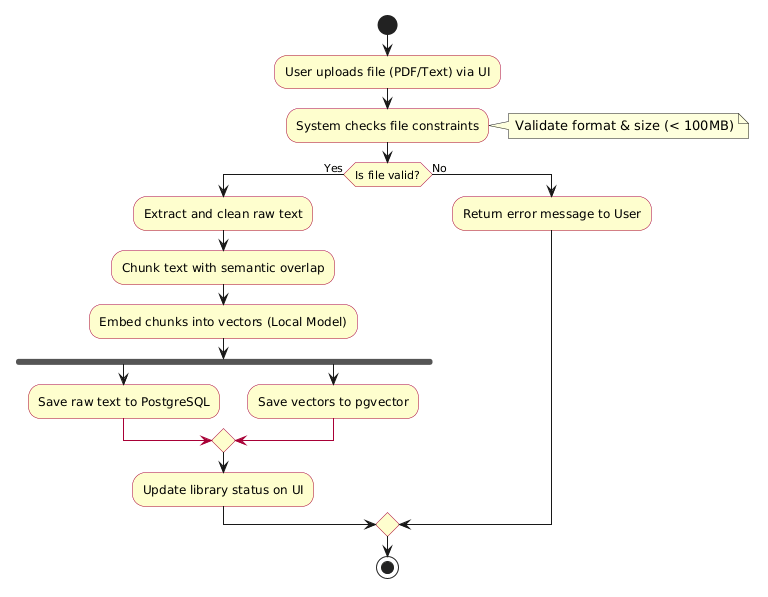
\includegraphics[width=0.92\linewidth]{images/activity-diagrams/ac-01.png}
\end{figure}

\begin{enumerate}
    \item Người dùng tải tệp PDF hoặc văn bản lên hệ thống thông qua giao diện.
    \item Máy chủ kiểm tra dung lượng, định dạng trước khi tiếp nhận tệp, lưu vào kho đối tượng và trả về ngay mã chấp nhận.
    \item Worker trích xuất văn bản thô; nếu không có lớp văn bản (PDF quét ảnh), worker chuyển sang luồng OCR (không thể hiện chi tiết trong sơ đồ trên, xem đặc tả UC-07).
    \item Văn bản được chia thành các đoạn nhỏ có chồng lấp để bảo toàn ngữ cảnh giữa các phân đoạn.
    \item Từng phân đoạn được chuyển qua mô hình nhúng cục bộ để tạo vector biểu diễn.
    \item Nội dung gốc và vector tương ứng được lưu đồng thời vào PostgreSQL với \texttt{pgvector}. \cite{reimers2019sentence,pgvector2023}
\end{enumerate}

\subsection{Truy vấn và phản hồi RAG}
Quy trình này mô tả cách hệ thống xử lý một câu hỏi để tạo phản hồi dựa trên ngữ cảnh tài liệu (UC-13, UC-14).

\begin{figure}[H]
    \centering
    \caption{Sơ đồ hoạt động của quy trình truy vấn và phản hồi RAG}
    \label{fig:activity-rag}
    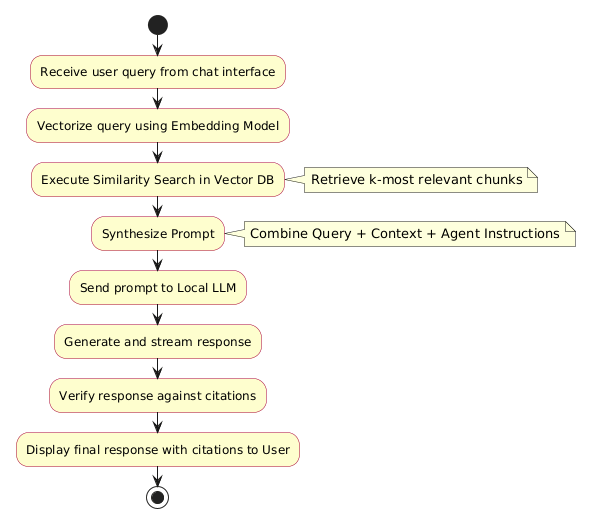
\includegraphics[width=0.88\linewidth]{images/activity-diagrams/ac-02.png}
\end{figure}

\begin{enumerate}
    \item Hệ thống tiếp nhận câu hỏi từ khung chat.
    \item Câu hỏi được nhúng hóa thành vector bằng cùng mô hình đã dùng ở giai đoạn lập chỉ mục.
    \item Hệ thống truy xuất các phân đoạn có độ liên quan cao nhất trong cơ sở dữ liệu vector.
    \item Câu hỏi, ngữ cảnh cứng (đoạn văn bản được chọn, nếu có) và ngữ cảnh truy xuất được ghép lại thành lời nhắc hoàn chỉnh cho bộ định tuyến LLM.
    \item Nhà cung cấp LLM khả dụng đầu tiên sinh phản hồi theo luồng (streaming).
    \item Hệ thống gửi trích dẫn nguồn kèm phản hồi cho giao diện hiển thị. \cite{lewis2020retrieval,gao2023retrieval}
\end{enumerate}

\subsection{Quản lý tài nguyên và dọn dẹp dữ liệu}
Quy trình này bảo đảm dữ liệu luôn nhất quán khi người dùng xóa tài liệu (UC-06).

\begin{figure}[H]
    \centering
    \caption{Sơ đồ hoạt động của quy trình quản lý tài nguyên và dọn dẹp dữ liệu}
    \label{fig:activity-cleanup}
    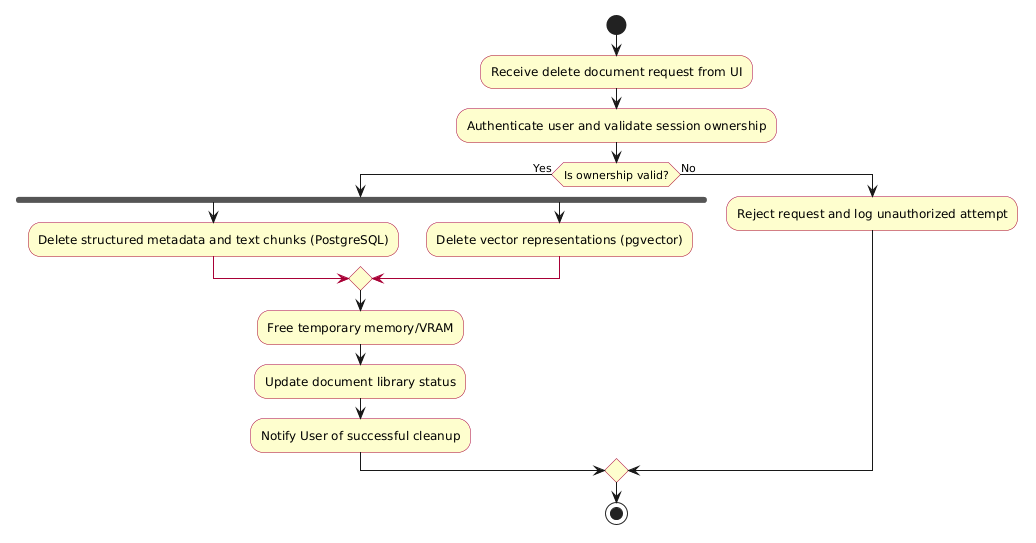
\includegraphics[width=0.96\linewidth]{images/activity-diagrams/ac-04.png}
\end{figure}

\begin{enumerate}
    \item Người dùng chọn hành động xóa tài liệu trong thư viện.
    \item Máy chủ kiểm tra quyền sở hữu (\texttt{user\_id}) trước khi thực hiện.
    \item Hệ thống xóa tệp vật lý khỏi kho lưu trữ đối tượng và phát lệnh xóa đến PostgreSQL.
    \item Cơ sở dữ liệu xóa tuần tự (cascade) các bản ghi liên quan: phân đoạn, vector, highlight và lịch sử hội thoại gắn với tài liệu.
    \item Giao diện cập nhật lại thư viện tài liệu sau khi quy trình hoàn tất. \cite{pgvector2023}
\end{enumerate}


\section{Sơ đồ trình tự}
Phần này mô tả trình tự tương tác giữa người dùng, giao diện, máy chủ điều phối và các dịch vụ AI. Các sơ đồ làm rõ cách hệ thống điều phối phiên, xử lý tài liệu và truy vấn RAG theo từng tình huống sử dụng. \cite{lewis2020retrieval}

\subsection{Quy trình quản trị phiên và khởi tạo không gian làm việc}

\begin{figure}[H]
    \centering
    \caption{Sơ đồ trình tự của quy trình quản trị phiên và khởi tạo không gian làm việc}
    \label{fig:sequence-session}
    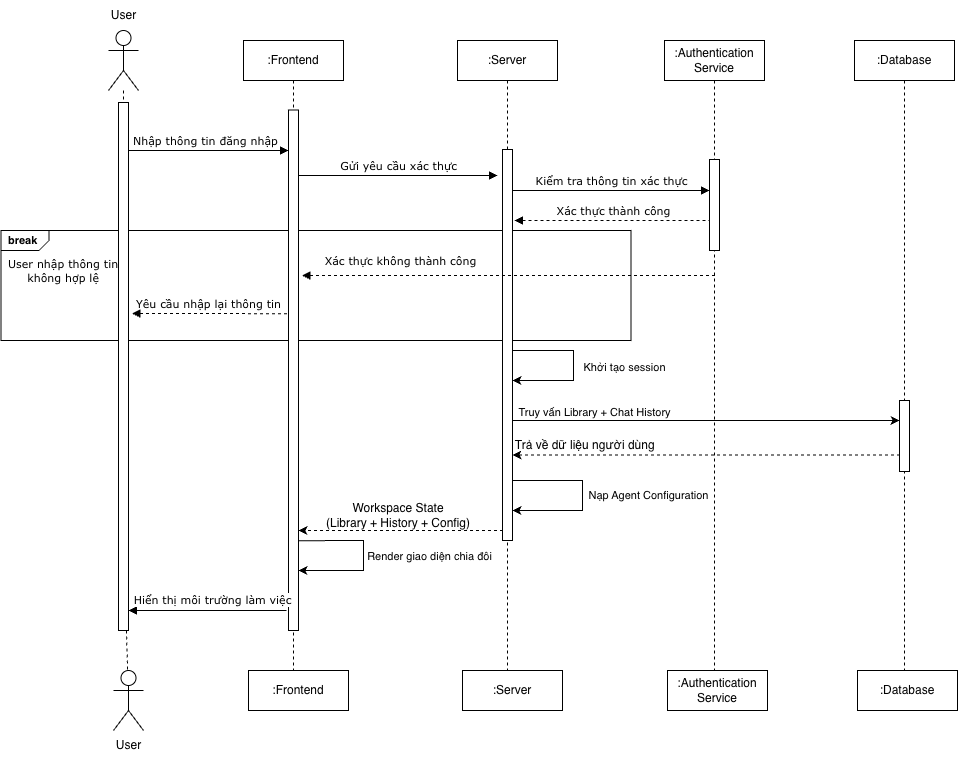
\includegraphics[width=\linewidth]{images/sequence-diagrams/seq-01.png}
\end{figure}

\begin{enumerate}
    \item Giao diện tiếp nhận thông tin xác thực từ người dùng và chuyển tiếp đến máy chủ điều phối.
    \item Máy chủ xác thực và cấp token phiên khi đăng nhập thành công (UC-02).
    \item Máy chủ truy vấn PostgreSQL để lấy danh sách workspace và tài liệu đã nạp.
    \item Cơ sở dữ liệu trả về trạng thái tài liệu và lịch sử hội thoại gần nhất.
    \item Máy chủ gửi toàn bộ trạng thái không gian làm việc về giao diện.
    \item Giao diện dựng màn hình thư viện và danh sách phiên chat.
\end{enumerate}

\subsection{Quy trình quản lý vòng đời và tiền xử lý tài liệu}

\begin{figure}[H]
    \centering
    \caption{Sơ đồ trình tự của quy trình quản lý vòng đời và tiền xử lý tài liệu}
    \label{fig:sequence-preprocess}
    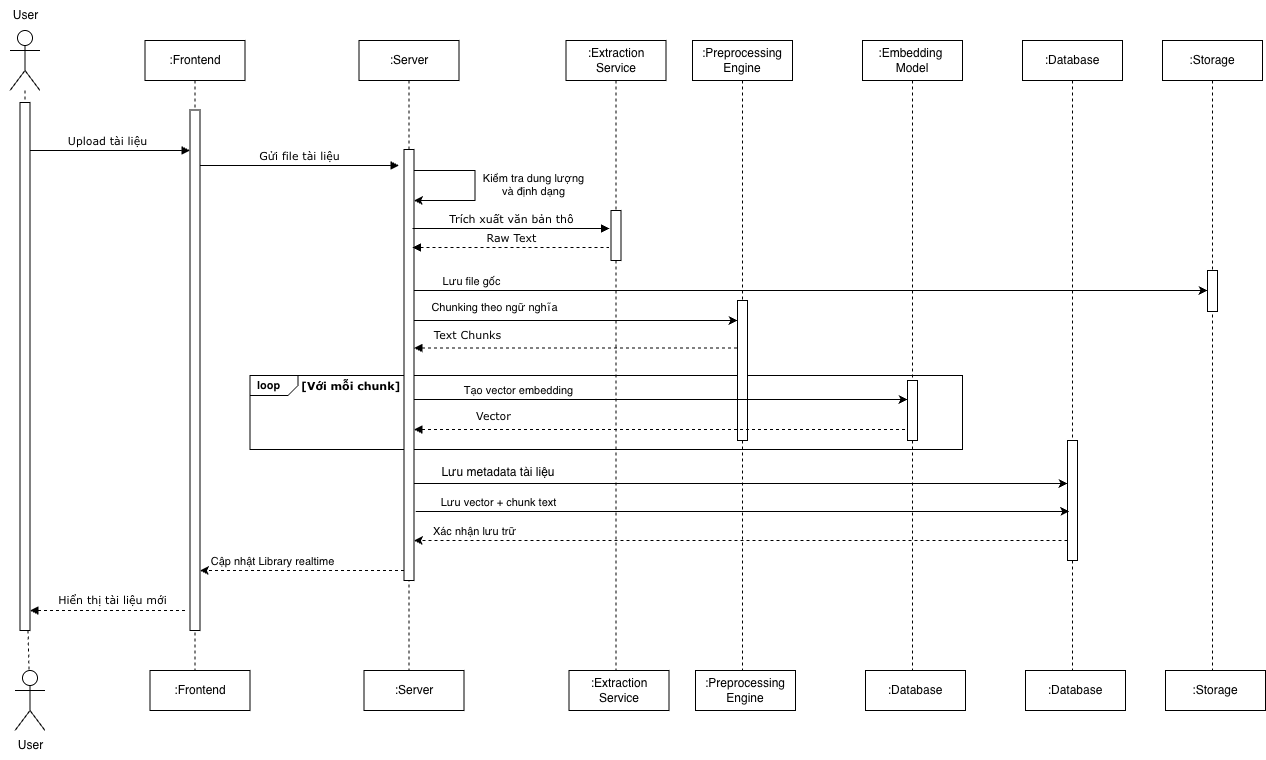
\includegraphics[width=\linewidth]{images/sequence-diagrams/seq-02.png}
\end{figure}

\begin{enumerate}
    \item Người dùng tải tệp tin thông qua giao diện (UC-05).
    \item Máy chủ tiếp nhận tệp, kiểm tra ràng buộc dung lượng/định dạng và trả về ngay mã chấp nhận.
    \item Worker (chạy nền, xem UC-07) gọi dịch vụ trích xuất để bóc tách văn bản và lưu tệp gốc vào kho đối tượng.
    \item Văn bản thô được chuyển đến bộ phân đoạn để chia theo ranh giới cấu trúc và ngữ nghĩa.
    \item Với mỗi phân đoạn, worker gọi dịch vụ nhúng để tạo vector đại diện.
    \item Worker ghi siêu dữ liệu và vector vào PostgreSQL với \texttt{pgvector}.
    \item Giao diện nhận cập nhật trạng thái và làm mới thư viện theo thời gian thực. \cite{reimers2019sentence,pgvector2023}
\end{enumerate}

\subsection{Quy trình hỏi đáp RAG và định tuyến LLM}

\begin{figure}[H]
    \centering
    \caption{Sơ đồ trình tự của quy trình hỏi đáp RAG và định tuyến LLM}
    \label{fig:sequence-rag}
    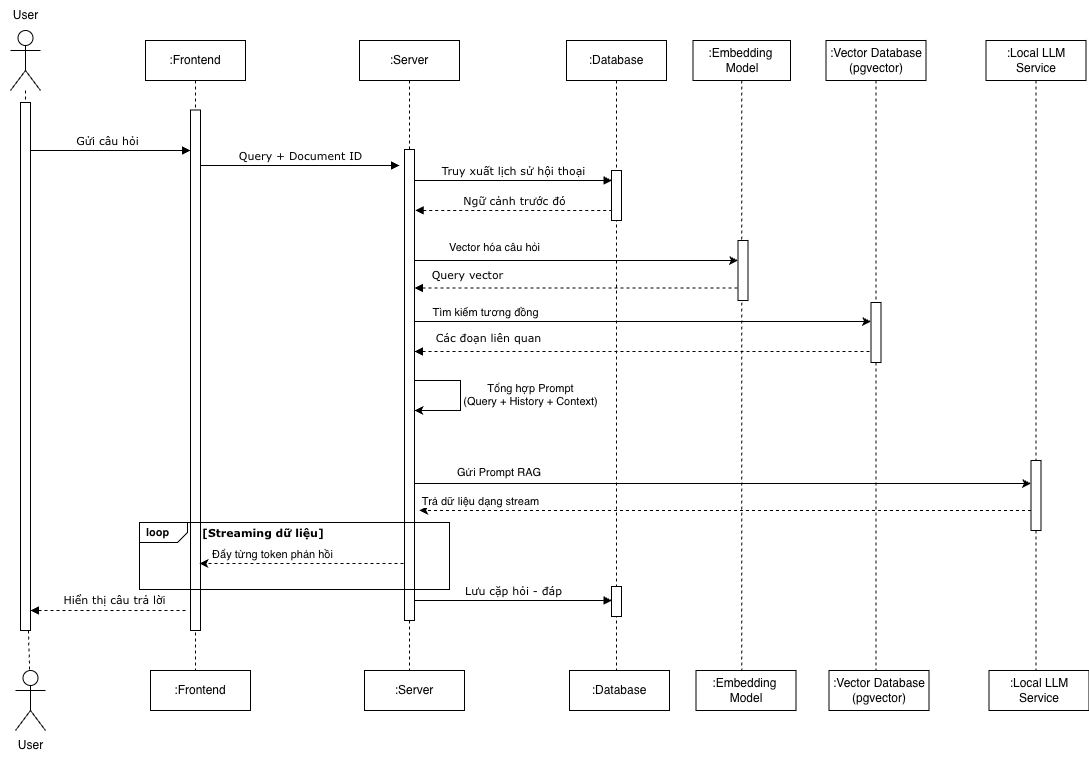
\includegraphics[width=\linewidth]{images/sequence-diagrams/seq-03.png}
\end{figure}

\begin{enumerate}
    \item Người dùng gửi câu hỏi từ khung chat cùng định danh tài liệu mục tiêu (UC-13/UC-14).
    \item Máy chủ truy vấn lịch sử hội thoại của phiên hiện tại để lấy ngữ cảnh trước đó.
    \item Câu hỏi hiện tại được nhúng hóa thành vector truy vấn.
    \item PostgreSQL với \texttt{pgvector} thực hiện tìm kiếm tương đồng và trả về các phân đoạn liên quan nhất.
    \item Máy chủ tổng hợp câu hỏi, ngữ cảnh cứng (nếu có đoạn văn bản được chọn), lịch sử hội thoại và các phân đoạn truy xuất thành một lời nhắc hoàn chỉnh.
    \item Máy chủ gửi lời nhắc đến nhà cung cấp LLM khả dụng đầu tiên trong danh sách ưu tiên của bộ định tuyến (nhãn ``Local LLM Service'' trong sơ đồ đại diện cho bộ định tuyến đa nhà cung cấp thực tế, xem Chương 5).
    \item Máy chủ vừa truyền dữ liệu theo luồng về giao diện, vừa lưu cặp hỏi--đáp mới vào lịch sử phiên. \cite{lewis2020retrieval,gao2023retrieval}
\end{enumerate}


\section{Thiết kế cấu trúc phần mềm (Sơ đồ lớp)}
Thiết kế cấu trúc phần mềm của DigitalBookLLM được xây dựng theo định hướng hướng đối tượng kết hợp với kiến trúc dịch vụ gọn nhẹ (modular monolith). Các lớp được chia thành bốn nhóm cốt lõi nhằm phân tách rõ ràng trách nhiệm giữa lưu trữ dữ liệu, điều phối nghiệp vụ, xử lý AI và quản lý trạng thái giao diện.

\begin{figure}[H]
    \centering
    \caption{Tổng quan sơ đồ lớp}
    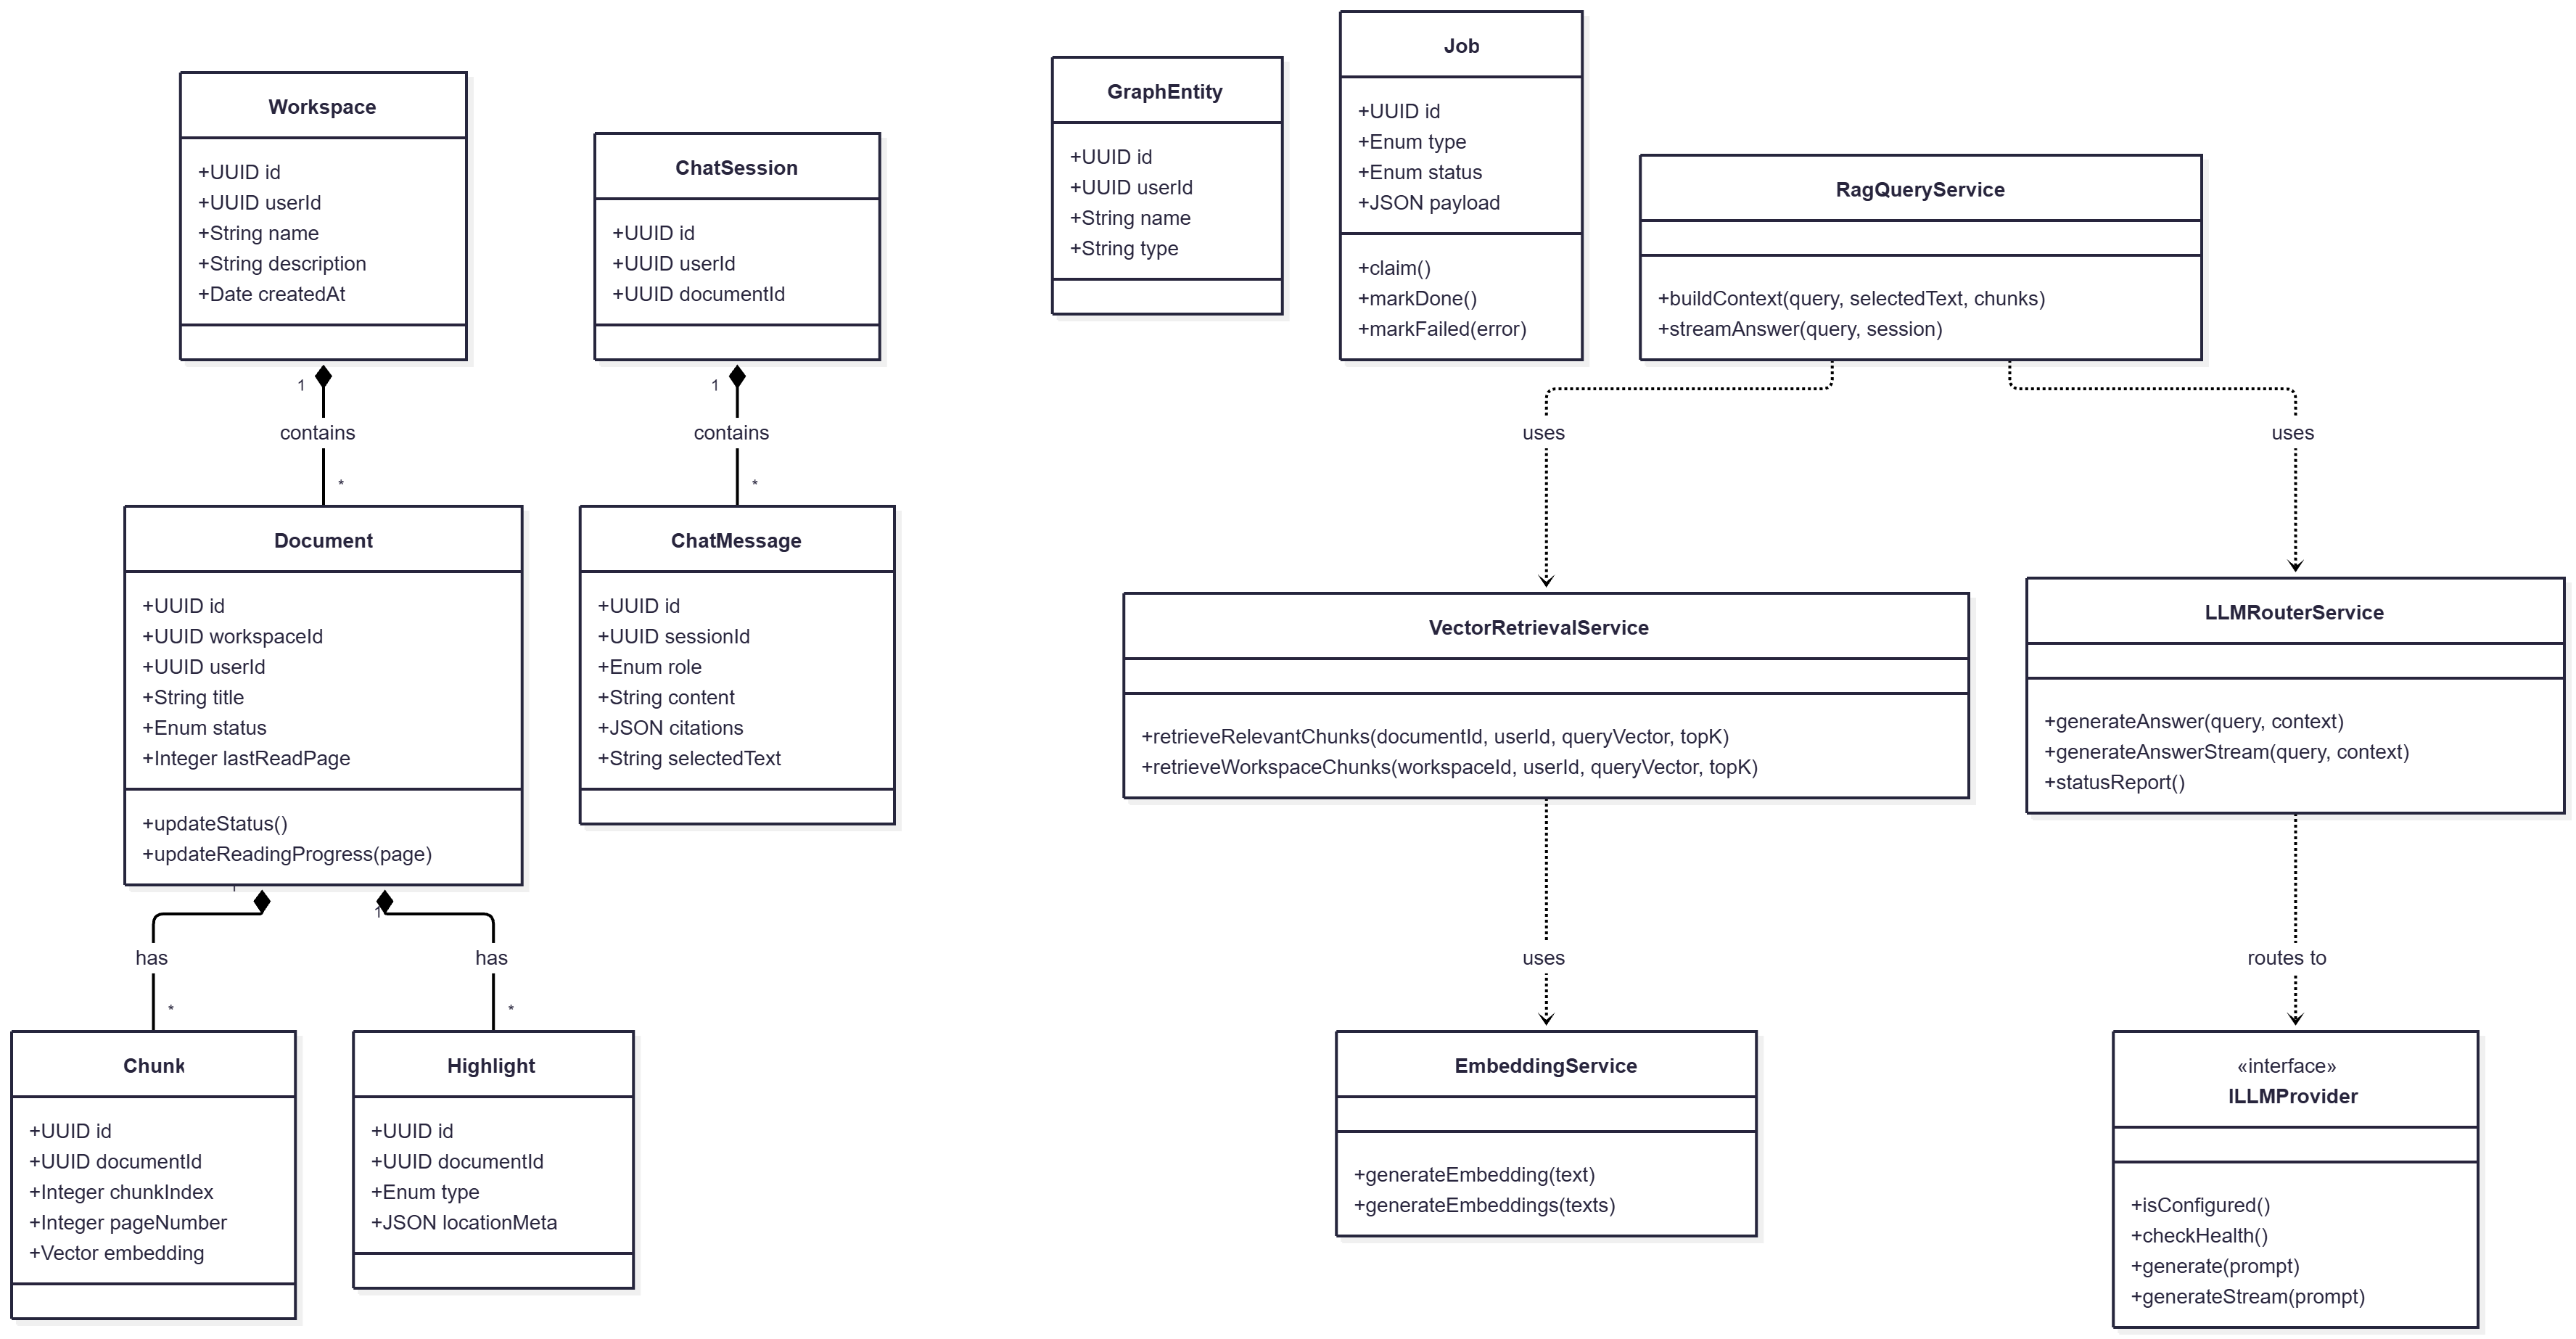
\includegraphics[width=\textwidth]{images/class_diagram.png}
    \label{fig:class}
\end{figure}

\subsection{Nhóm lớp thực thể và quản lý dữ liệu}
Nhóm lớp này ánh xạ cấu trúc dữ liệu bền vững từ PostgreSQL lên bộ nhớ ứng dụng.

\subsubsection{Lớp \texttt{Workspace} (Không gian làm việc)}
    \noindent\textbf{Vai trò:} Đơn vị tổ chức tài liệu độc lập, thuộc sở hữu của một người dùng.\\
    \textbf{Thuộc tính:} \texttt{id} (UUID), \texttt{userId} (UUID), \texttt{name} (String), \texttt{description} (String), \texttt{createdAt}, \texttt{updatedAt}.

\subsubsection{Lớp \texttt{Document} (Tài liệu)}
    \noindent\textbf{Vai trò:} Quản lý trạng thái vòng đời của một tài liệu từ khi được tải lên đến khi sẵn sàng phục vụ truy xuất.\\
    \textbf{Thuộc tính:}
    \begin{itemize}
        \item \texttt{id} (UUID), \texttt{workspaceId} (UUID), \texttt{userId} (UUID): định danh và quan hệ sở hữu.
        \item \texttt{title}, \texttt{author}, \texttt{fileType}, \texttt{fileSize}, \texttt{storageKey}, \texttt{coverKey}, \texttt{pageCount}.
        \item \texttt{status} (Enum: \texttt{UPLOADED}, \texttt{PROCESSING}, \texttt{READY}, \texttt{FAILED}), \texttt{ocrUsed} (Boolean), \texttt{lastReadPage} (Integer).
    \end{itemize}
    \textbf{Phương thức:} \texttt{updateStatus()}, \texttt{updateReadingProgress(page)}.

\subsubsection{Lớp \texttt{Chunk} (Phân đoạn tài liệu)}
    \noindent\textbf{Vai trò:} Biểu diễn đơn vị dữ liệu nhỏ nhất phục vụ tìm kiếm ngữ nghĩa.\\
    \textbf{Thuộc tính:} \texttt{id} (UUID), \texttt{documentId} (UUID), \texttt{chunkIndex} (Integer), \texttt{pageNumber} (Integer), \texttt{text} (Text), \texttt{embedding} (Vector[384]).

\subsubsection{Lớp \texttt{Highlight} (Đánh dấu và ghi chú)}
    \noindent\textbf{Vai trò:} Lưu vị trí và nội dung của một highlight hoặc bookmark do người dùng tạo (UC-10, UC-11).\\
    \textbf{Thuộc tính:} \texttt{id}, \texttt{documentId}, \texttt{userId}, \texttt{type} (Enum: \texttt{HIGHLIGHT}, \texttt{BOOKMARK}), \texttt{content}, \texttt{note}, \texttt{color}, \texttt{locationMeta} (JSON: trang + toạ độ chuẩn hoá).

\subsubsection{Lớp \texttt{ChatSession} và \texttt{ChatMessage}}
    \noindent\textbf{Vai trò:} Lưu vết từng lượt tương tác trong hội thoại giữa người dùng và trợ lý AI.\\
    \textbf{Thuộc tính (\texttt{ChatMessage}):} \texttt{id}, \texttt{sessionId}, \texttt{role} (Enum: \texttt{user}, \texttt{assistant}), \texttt{content}, \texttt{selectedText}, \texttt{citations} (JSON), \texttt{provider}.

\subsubsection{Lớp \texttt{GraphEntity} và \texttt{GraphRelation}}
    \noindent\textbf{Vai trò:} Biểu diễn nút và cạnh của đồ thị tri thức cá nhân (UC-15).\\
    \textbf{Thuộc tính (\texttt{GraphEntity}):} \texttt{id}, \texttt{userId}, \texttt{name}, \texttt{type}, \texttt{description}.\\
    \textbf{Thuộc tính (\texttt{GraphRelation}):} \texttt{id}, \texttt{sourceEntityId}, \texttt{targetEntityId}, \texttt{relationType}, \texttt{sourceDocumentId}, \texttt{excerpt}.

\subsubsection{Lớp \texttt{Job} (Tác vụ hàng đợi)}
    \noindent\textbf{Vai trò:} Đại diện cho một tác vụ nền (nạp tài liệu, trích xuất tri thức) trong hàng đợi bền vững.\\
    \textbf{Thuộc tính:} \texttt{id}, \texttt{type} (Enum: \texttt{INGEST\_DOCUMENT}, \texttt{EXTRACT\_ENTITIES}), \texttt{payload} (JSON), \texttt{status} (Enum: \texttt{PENDING}, \texttt{RUNNING}, \texttt{DONE}, \texttt{FAILED}, \texttt{DEAD}), \texttt{attempts}.\\
    \textbf{Phương thức:} \texttt{claim()}, \texttt{markDone()}, \texttt{markFailed(error)}.

\subsection{Nhóm lớp dịch vụ và điều phối}

\subsubsection{Lớp \texttt{VectorRetrievalService} (Dịch vụ truy xuất vector)}
    \noindent\textbf{Vai trò:} Thực hiện tìm kiếm tương đồng trên \texttt{pgvector}, luôn lọc theo \texttt{userId} để đảm bảo cô lập dữ liệu (NFR-04.1).\\
    \textbf{Phương thức:}
    \begin{itemize}
        \item \texttt{retrieveRelevantChunks(documentId, userId, queryVector, topK)}: tìm kiếm trong phạm vi một tài liệu.
        \item \texttt{retrieveWorkspaceChunks(workspaceId, userId, queryVector, topK)}: tìm kiếm trong toàn bộ không gian làm việc.
    \end{itemize}

\subsubsection{Lớp \texttt{RagQueryService} (Dịch vụ điều phối truy vấn RAG)}
    \noindent\textbf{Vai trò:} Điều phối một lượt hỏi đáp: truy xuất ngữ cảnh, xây dựng lời nhắc, gọi bộ định tuyến LLM và lưu lại lịch sử.\\
    \textbf{Phương thức:}
    \begin{itemize}
        \item \texttt{buildContext(query, selectedText, chunks)}: ghép ngữ cảnh cứng (nếu có) và các phân đoạn truy xuất thành lời nhắc.
        \item \texttt{streamAnswer(query, session)}: thực thi luồng xử lý từ truy xuất đến phát sinh câu trả lời dạng streaming (SSE).
    \end{itemize}

\subsection{Nhóm lớp AI và xử lý ngôn ngữ}
Nhóm này bao bọc các lời gọi đến các nhà cung cấp LLM bên ngoài, áp dụng nguyên tắc phụ thuộc lỏng (dependency inversion) để có thể thay thế hoặc thêm nhà cung cấp mà không ảnh hưởng đến phần còn lại của hệ thống.

\subsubsection{Giao diện \texttt{ILLMProvider}}
    \noindent\textbf{Vai trò:} Xác định hợp đồng chuẩn cho mọi nhà cung cấp LLM được tích hợp vào hệ thống.\\
    \textbf{Phương thức trừu tượng:} \texttt{isConfigured()}, \texttt{checkHealth()}, \texttt{generate(prompt)}, \texttt{generateStream(prompt)}.

\subsubsection{Lớp \texttt{LLMRouterService} (Bộ định tuyến LLM)}
    \noindent\textbf{Vai trò:} Giữ danh sách nhà cung cấp theo thứ tự ưu tiên, dò trạng thái khả dụng và định tuyến yêu cầu đến nhà cung cấp còn hoạt động đầu tiên, tự động chuyển sang nhà cung cấp kế tiếp nếu gặp lỗi.\\
    \textbf{Phương thức:} \texttt{generateAnswer(query, context)}, \texttt{generateAnswerStream(query, context)}, \texttt{statusReport()}.\\
    \textbf{Lớp hiện thực \texttt{ILLMProvider}:} \texttt{OpenAiCompatibleProvider} (dùng chung cho các API tương thích chuẩn OpenAI), \texttt{AnthropicProvider}, \texttt{GeminiProvider}.

\subsubsection{Lớp \texttt{EmbeddingService} (Dịch vụ nhúng)}
    \noindent\textbf{Vai trò:} Chuyển đổi văn bản thành vector số thực để phục vụ truy xuất ngữ nghĩa, chạy cục bộ (không phụ thuộc API bên ngoài).\\
    \textbf{Phương thức:} \texttt{generateEmbedding(text)}, \texttt{generateEmbeddings(texts)}.

\subsection{Nhóm thành phần giao diện động}
Mặc dù giao diện được hiện thực bằng mô hình thành phần hàm của React/Next.js, việc mô tả các thực thể quản lý trạng thái chính vẫn cần thiết để làm rõ cách hệ thống tổ chức tương tác người dùng.

\subsubsection{Lớp \texttt{WorkspaceController} (Bộ điều khiển không gian)}
    \noindent\textbf{Vai trò:} Quản lý trạng thái chung của toàn bộ không gian làm việc.\\
    \textbf{Thuộc tính:} \texttt{activeDocument}, \texttt{isProcessing}, \texttt{viewMode} (\texttt{reading}/\texttt{split}/\texttt{graph}).\\
    \textbf{Phương thức:} \texttt{loadWorkspaceState()}.

\subsubsection{Lớp \texttt{DocumentViewer} (Trình hiển thị tài liệu)}
    \noindent\textbf{Vai trò:} Kết xuất trực quan tài liệu gốc theo cơ chế windowed rendering (FR-08) và hỗ trợ điều hướng theo trích dẫn.\\
    \textbf{Phương thức:} \texttt{renderPage(pageNumber)}, \texttt{scrollToCitation(page)}, \texttt{onTextSelect(callback)}.

\subsubsection{Lớp \texttt{ChatPanel} (Bảng tương tác)}
    \noindent\textbf{Vai trò:} Quản lý luồng hội thoại và hiển thị phản hồi theo thời gian thực.\\
    \textbf{Thuộc tính:} \texttt{messageList}, \texttt{isStreaming}, \texttt{selectedTextContext}.\\
    \textbf{Phương thức:} \texttt{appendStreamChunk()}, \texttt{renderCitations()}.


\section{Thiết kế cơ sở dữ liệu}
Thiết kế cơ sở dữ liệu của DigitalBookLLM được xây dựng trên PostgreSQL kết hợp phần mở rộng \texttt{pgvector}. Mục tiêu là lưu trữ tập trung tại máy chủ toàn bộ tài liệu, phân mảnh văn bản, vector nhúng, highlight, phiên hội thoại, đồ thị tri thức và hàng đợi tác vụ, đồng thời bảo đảm dữ liệu của từng người dùng được cách ly và có thể dọn dẹp nhất quán khi tài liệu bị xóa (ADR-02, ADR-03, ADR-04, xem Chương 5).

\subsection{Nguyên tắc thiết kế dữ liệu}
Lược đồ dữ liệu tuân theo ba nguyên tắc chính. Thứ nhất, mọi bảng chứa dữ liệu người dùng đều mang trực tiếp hoặc gián tiếp trường \texttt{user\_id}, làm cơ sở cho việc cô lập dữ liệu (NFR-04.1). Thứ hai, mọi dữ liệu phát sinh từ tài liệu (phân mảnh, vector, highlight, hội thoại) đều phụ thuộc khóa ngoại với ràng buộc xóa tuần tự (\texttt{ON DELETE CASCADE}). Thứ ba, cả vector nhúng lẫn đồ thị tri thức đều được lưu ngay trong PostgreSQL thay vì các hệ quản trị chuyên dụng riêng biệt, nhằm giảm độ phức tạp vận hành và tránh vấn đề nhất quán giữa nhiều kho dữ liệu.

\subsection{Mô hình quan hệ tổng quát}
Các bảng cốt lõi được tổ chức thành sáu nhóm: người dùng, không gian làm việc, tài liệu và phân mảnh, đánh dấu, hội thoại, đồ thị tri thức, và hàng đợi tác vụ.

\begin{longtable}{|C{0.18\linewidth}|L{0.28\linewidth}|L{0.36\linewidth}|}
\caption{Các bảng dữ liệu chính của DigitalBookLLM}\label{tab:database-tables}\\
\hline
\multicolumn{1}{|C{0.18\linewidth}|}{\textbf{Bảng}} & \multicolumn{1}{C{0.28\linewidth}|}{\textbf{Vai trò}} & \multicolumn{1}{C{0.36\linewidth}|}{\textbf{Dữ liệu chính}} \\\hline
\endfirsthead
\hline
\multicolumn{1}{|C{0.18\linewidth}|}{\textbf{Bảng}} & \multicolumn{1}{C{0.28\linewidth}|}{\textbf{Vai trò}} & \multicolumn{1}{C{0.36\linewidth}|}{\textbf{Dữ liệu chính}} \\\hline
\endhead
\texttt{users} & Quản lý danh tính và ranh giới dữ liệu. & Email, mật khẩu băm, thời điểm tạo. \\\hline
\texttt{workspaces} & Không gian làm việc độc lập của người dùng. & Tên, mô tả, chủ sở hữu. \\\hline
\texttt{documents} & Quản lý metadata và trạng thái xử lý của tài liệu. & Tiêu đề, loại tệp, khóa lưu trữ, trạng thái, trang đang đọc. \\\hline
\texttt{chunks} & Lưu phân mảnh văn bản và vector nhúng phục vụ RAG. & Nội dung, số trang, thứ tự phân mảnh, vector 384 chiều. \\\hline
\texttt{highlights} & Lưu highlight và bookmark. & Loại, nội dung, ghi chú, màu, toạ độ vị trí (JSON). \\\hline
\texttt{chat\_sessions}, \texttt{chat\_messages} & Ghi lại lịch sử hội thoại. & Vai trò tin nhắn, nội dung, trích dẫn (JSON), nhà cung cấp LLM. \\\hline
\texttt{entities}, \texttt{entity\_relations} & Đồ thị tri thức cá nhân. & Tên/loại thực thể; quan hệ, tài liệu nguồn, đoạn trích. \\\hline
\texttt{jobs} & Hàng đợi tác vụ nền bền vững. & Loại tác vụ, payload, trạng thái, số lần thử lại. \\\hline
\end{longtable}

\subsection{Đặc tả bảng dữ liệu}
Bảng \ref{tab:database-schema} mô tả các trường dữ liệu quan trọng nhất trong lược đồ. Kiểu \texttt{vector} do \texttt{pgvector} cung cấp, cấu hình 384 chiều tương ứng với mô hình nhúng \texttt{all-MiniLM-L6-v2}.

\begin{longtable}{|C{0.16\linewidth}|L{0.24\linewidth}|C{0.14\linewidth}|L{0.28\linewidth}|}
\caption{Đặc tả lược đồ cơ sở dữ liệu (trích các trường trọng tâm)}\label{tab:database-schema}\\
\hline
\multicolumn{1}{|C{0.16\linewidth}|}{\textbf{Bảng}} & \multicolumn{1}{C{0.24\linewidth}|}{\textbf{Trường}} & \multicolumn{1}{C{0.14\linewidth}|}{\textbf{Kiểu}} & \multicolumn{1}{C{0.28\linewidth}|}{\textbf{Ràng buộc}} \\\hline
\endfirsthead
\hline
\multicolumn{1}{|C{0.16\linewidth}|}{\textbf{Bảng}} & \multicolumn{1}{C{0.24\linewidth}|}{\textbf{Trường}} & \multicolumn{1}{C{0.14\linewidth}|}{\textbf{Kiểu}} & \multicolumn{1}{C{0.28\linewidth}|}{\textbf{Ràng buộc}} \\\hline
\endhead
\texttt{users} & \texttt{id} & VARCHAR & Khóa chính (UUID). \\\hline
\texttt{workspaces} & \texttt{user\_id} & VARCHAR & Khóa ngoại đến \texttt{users(id)}, xóa tuần tự. \\\hline
\texttt{documents} & \texttt{status} & Enum & \texttt{UPLOADED}, \texttt{PROCESSING}, \texttt{READY}, \texttt{FAILED}. \\\hline
\texttt{documents} & \texttt{storage\_key}, \texttt{cover\_key} & VARCHAR & Khóa đối tượng trong kho lưu trữ tệp. \\\hline
\texttt{chunks} & \texttt{embedding} & Vector(384) & Vector nhúng dùng cho tìm kiếm tương đồng. \\\hline
\texttt{chunks} & \texttt{page\_number} & Integer & Hỗ trợ trích dẫn trỏ ngược đến đúng trang. \\\hline
\texttt{highlights} & \texttt{type} & Enum & \texttt{HIGHLIGHT}, \texttt{BOOKMARK}. \\\hline
\texttt{highlights} & \texttt{location\_meta} & JSONB & Số trang và toạ độ vùng chọn chuẩn hoá (0--1). \\\hline
\texttt{chat\_messages} & \texttt{citations} & JSONB & Danh sách đoạn trích, số trang và độ tương đồng. \\\hline
\texttt{entities} & \texttt{user\_id}, \texttt{name} & VARCHAR & Ràng buộc duy nhất theo cặp (tránh trùng thực thể). \\\hline
\texttt{entity\_relations} & \texttt{source\_entity\_id}, \texttt{target\_entity\_id} & VARCHAR & Khóa ngoại đến \texttt{entities(id)}, xóa tuần tự. \\\hline
\texttt{jobs} & \texttt{status} & Enum & \texttt{PENDING}, \texttt{RUNNING}, \texttt{DONE}, \texttt{FAILED}, \texttt{DEAD}. \\\hline
\end{longtable}

\subsection{Ràng buộc toàn vẹn và xóa tuần tự}
Các quan hệ phụ thuộc được thiết kế theo hướng một chiều từ người dùng đến không gian làm việc, tài liệu, phân mảnh, highlight và hội thoại. Khi một tài liệu bị xóa, cơ sở dữ liệu tự động xóa các bản ghi trong \texttt{chunks}, \texttt{highlights} và các tin nhắn liên quan trong \texttt{chat\_messages}. Cách thiết kế này đáp ứng UC-06 và tránh để lại vector mồ côi trong kho dữ liệu.

\subsection{Chỉ mục và truy xuất vector}
Bảng \texttt{chunks} cần hai nhóm chỉ mục: B-tree trên \texttt{document\_id}/\texttt{user\_id} để lọc dữ liệu theo phạm vi sở hữu, và chỉ mục vector HNSW trên trường \texttt{embedding} để tăng tốc tìm kiếm tương đồng ngữ nghĩa (xem thuật toán HNSW ở Chương 2).

\begin{longtable}{|C{0.24\linewidth}|L{0.25\linewidth}|L{0.32\linewidth}|}
\caption{Chiến lược chỉ mục dữ liệu}\label{tab:database-indexes}\\
\hline
\multicolumn{1}{|C{0.24\linewidth}|}{\textbf{Chỉ mục}} & \multicolumn{1}{C{0.25\linewidth}|}{\textbf{Áp dụng cho}} & \multicolumn{1}{C{0.32\linewidth}|}{\textbf{Mục đích}} \\\hline
\endfirsthead
\hline
\multicolumn{1}{|C{0.24\linewidth}|}{\textbf{Chỉ mục}} & \multicolumn{1}{C{0.25\linewidth}|}{\textbf{Áp dụng cho}} & \multicolumn{1}{C{0.32\linewidth}|}{\textbf{Mục đích}} \\\hline
\endhead
B-tree theo \texttt{user\_id} & \texttt{documents}, \texttt{chunks}, \texttt{highlights}, \texttt{entities} & Cách ly dữ liệu và tăng tốc truy vấn theo người dùng. \\\hline
B-tree theo \texttt{document\_id} & \texttt{chunks}, \texttt{highlights} & Lọc phân mảnh và highlight theo tài liệu đang mở. \\\hline
HNSW index & \texttt{chunks.embedding} & Tìm kiếm các phân mảnh gần nhất trong không gian ngữ nghĩa (vector\_cosine\_ops). \\\hline
Partial index theo \texttt{status} & \texttt{jobs} & Tăng tốc truy vấn tác vụ đang chờ (\texttt{PENDING}/\texttt{RUNNING}). \\\hline
\end{longtable}

\subsection{Luồng dữ liệu lưu trữ}
Khi người dùng tải tài liệu lên, hệ thống tạo một bản ghi trong \texttt{documents} với trạng thái \texttt{UPLOADED} và một bản ghi trong \texttt{jobs}. Worker giành quyền xử lý tác vụ, chuyển trạng thái tài liệu sang \texttt{PROCESSING}; từng phân mảnh được ghi vào \texttt{chunks} cùng vector nhúng. Khi hoàn tất, trạng thái tài liệu chuyển sang \texttt{READY} và một tác vụ trích xuất tri thức mới được đưa vào \texttt{jobs}. Trong quá trình hỏi đáp, mỗi câu hỏi và phản hồi được lưu vào \texttt{chat\_messages} kèm trích dẫn liên kết tới phân mảnh nguồn, đồng thời một tác vụ trích xuất thực thể được đưa vào hàng đợi để cập nhật đồ thị tri thức.


\section{Thiết kế UI và UX}
Thiết kế UI và UX của DigitalBookLLM không chỉ phục vụ mục tiêu thẩm mỹ mà còn là một phần của lời giải kỹ thuật cho bài toán đứt gãy ngữ cảnh khi làm việc với tài liệu dài. Toàn bộ giao diện được xây dựng theo hướng ưu tiên không gian đọc, khả năng tương tác trực tiếp với tài liệu và phản hồi theo thời gian thực.

\subsection{Nguyên tắc thiết kế cốt lõi}
Giao diện của hệ thống được xây dựng theo triết lý \textit{knowledge-centric design}, tức là ưu tiên tối đa cho không gian đọc, suy luận và tương tác với tài liệu.

\begin{itemize}
    \item \textbf{Tính nhất quán về ngữ cảnh.} Luôn duy trì sự hiện diện song song của tài liệu gốc và cửa sổ hội thoại.
    \item \textbf{Phản hồi tức thì.} Sử dụng cơ chế streaming để hiển thị câu trả lời ngay trong khi mô hình đang suy luận.
    \item \textbf{Tương tác hai chiều.} Không chỉ người dùng đặt câu hỏi cho AI, mà AI còn có khả năng điều hướng người dùng quay trở lại đúng vị trí trong tài liệu thông qua hệ thống trích dẫn.
\end{itemize}

\subsection{Đặc tả các màn hình chức năng chính}
\subsubsection{Màn hình thư viện tri thức}
Đây là nơi người dùng quản lý các tài liệu đã nạp vào hệ thống. UI cần thể hiện được tính trực quan và trạng thái xử lý của từng tệp.

\begin{figure}[H]
    \centering
    \caption{Giao diện thư viện tri thức của hệ thống}
    \label{fig:ui-library}
    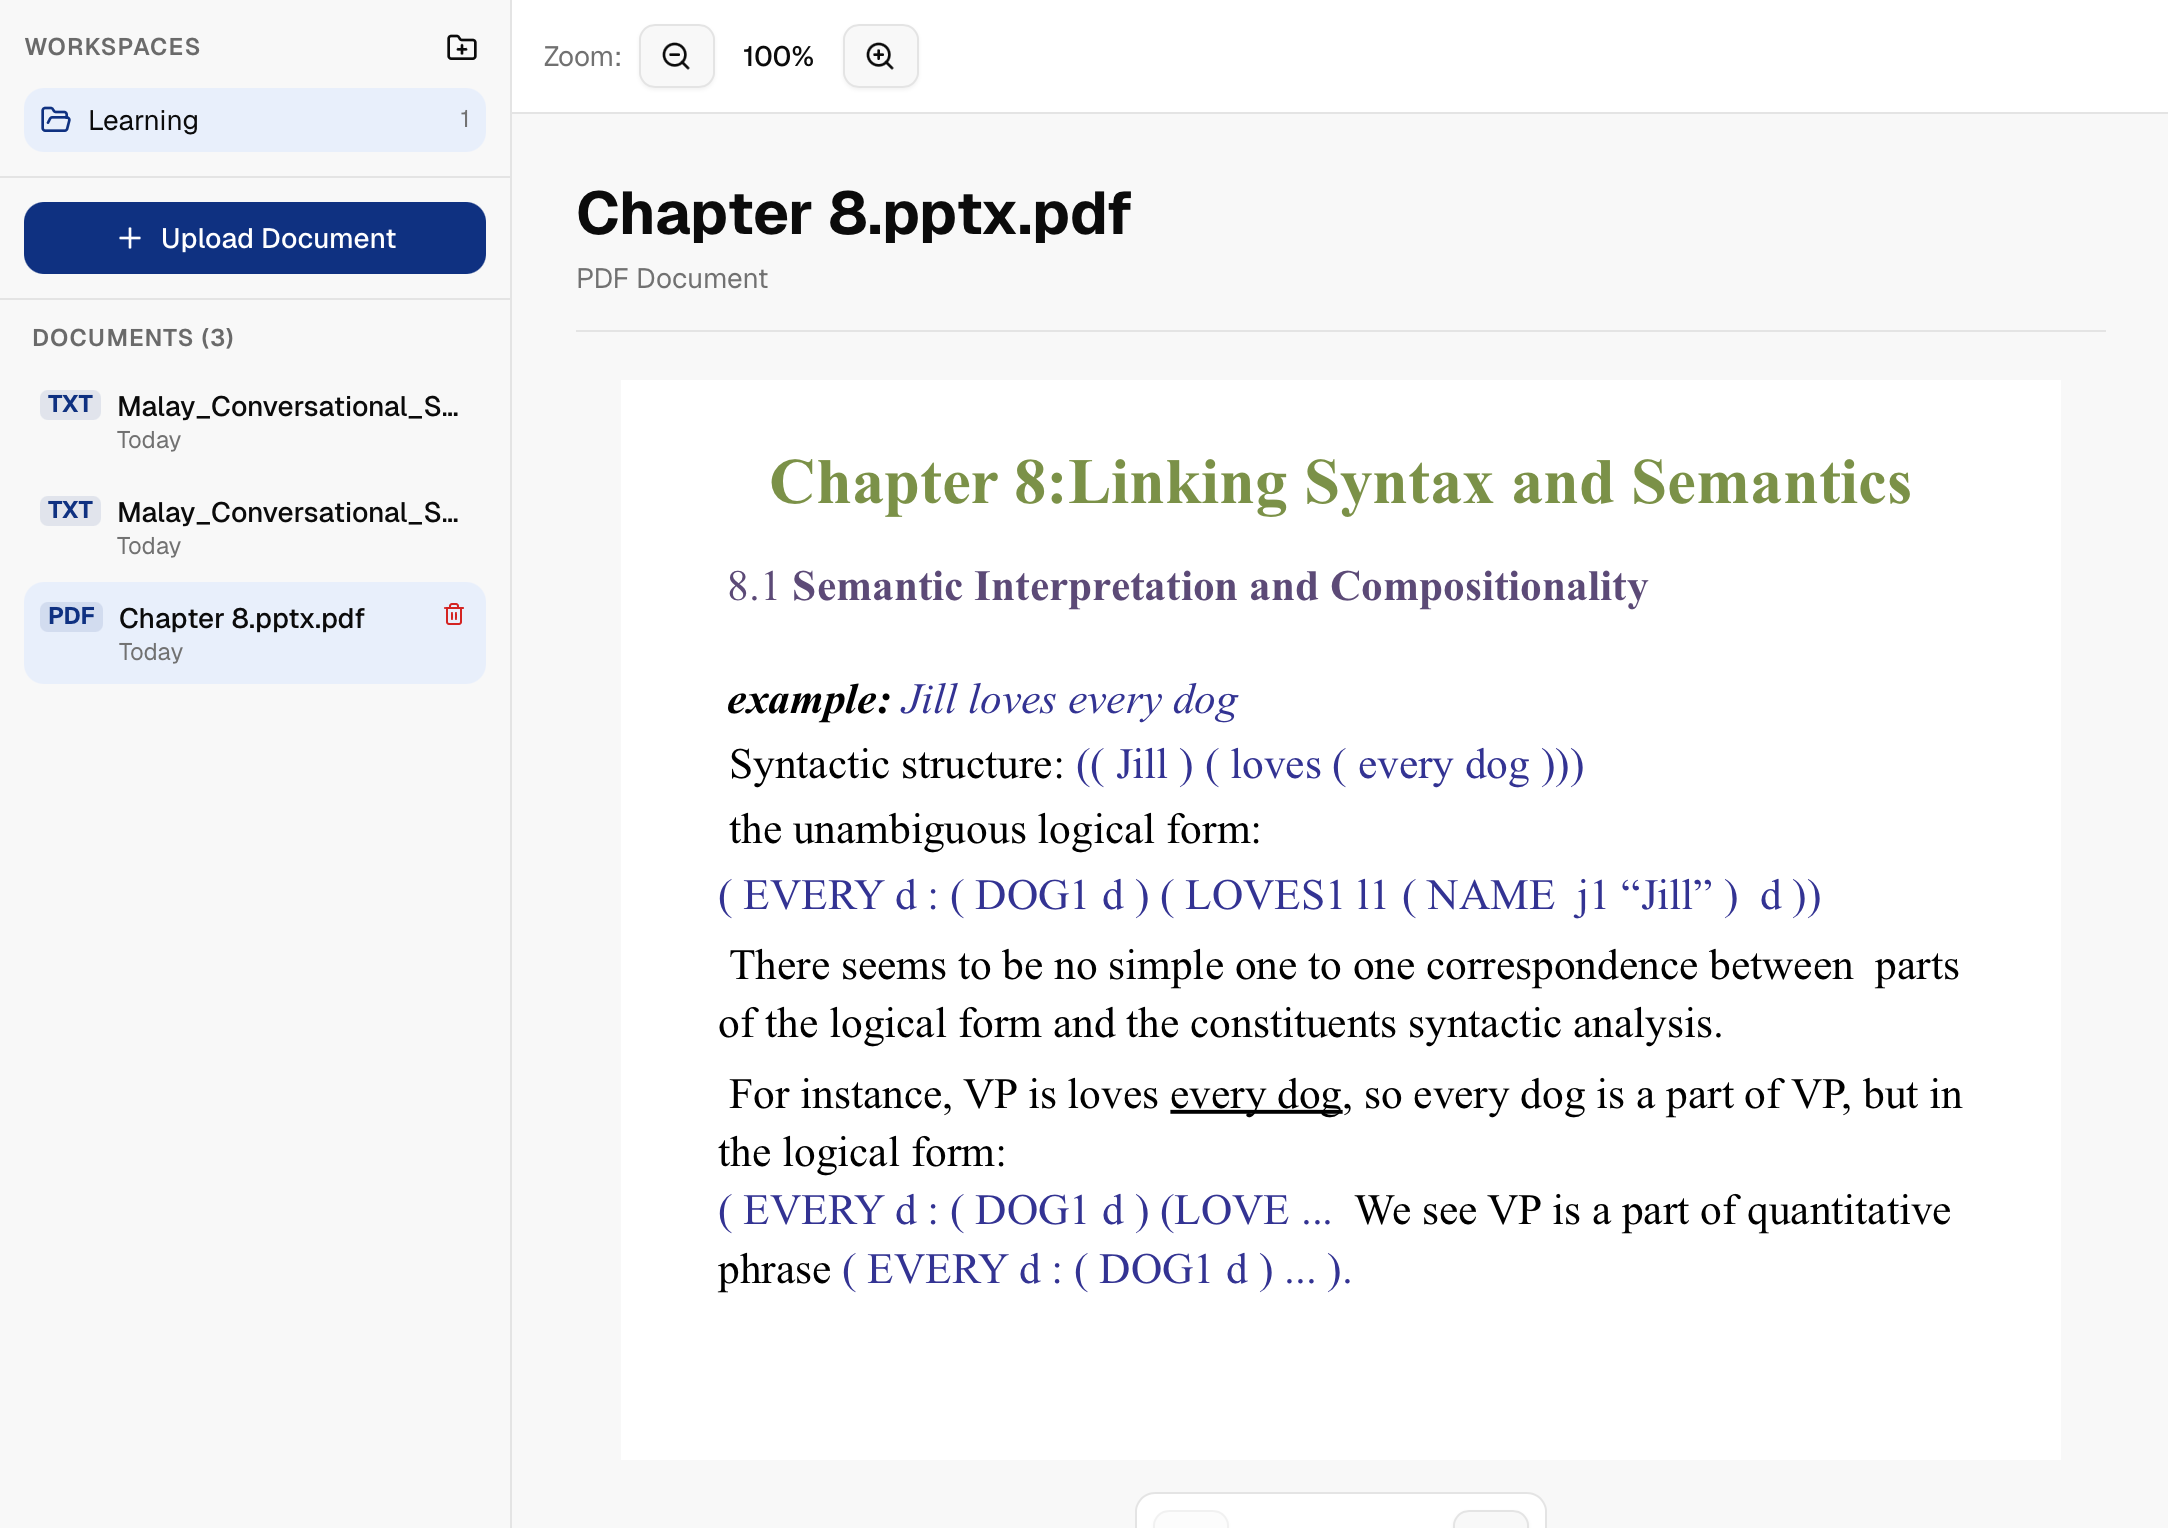
\includegraphics[width=0.88\linewidth]{images/ui-ux/workspace.png}
\end{figure}

\begin{itemize}
    \item \textbf{Nội dung chính.} Hiển thị danh sách tài liệu dưới dạng lưới hoặc danh sách; mỗi thẻ tài liệu bao gồm tên, kích thước, ngày nạp và trạng thái xử lý.
    \item \textbf{Mục tiêu sử dụng.} Giúp người dùng quan sát nhanh toàn bộ thư viện và chọn đúng tài liệu để tiếp tục làm việc.
\end{itemize}

\subsubsection{Không gian làm việc chia đôi}
Đây là giao diện quan trọng nhất, nơi diễn ra tương tác RAG theo thời gian thực.

\begin{figure}[H]
    \centering
    \caption{Giao diện không gian làm việc chia đôi giữa tài liệu và hội thoại}
    \label{fig:ui-split-screen}
    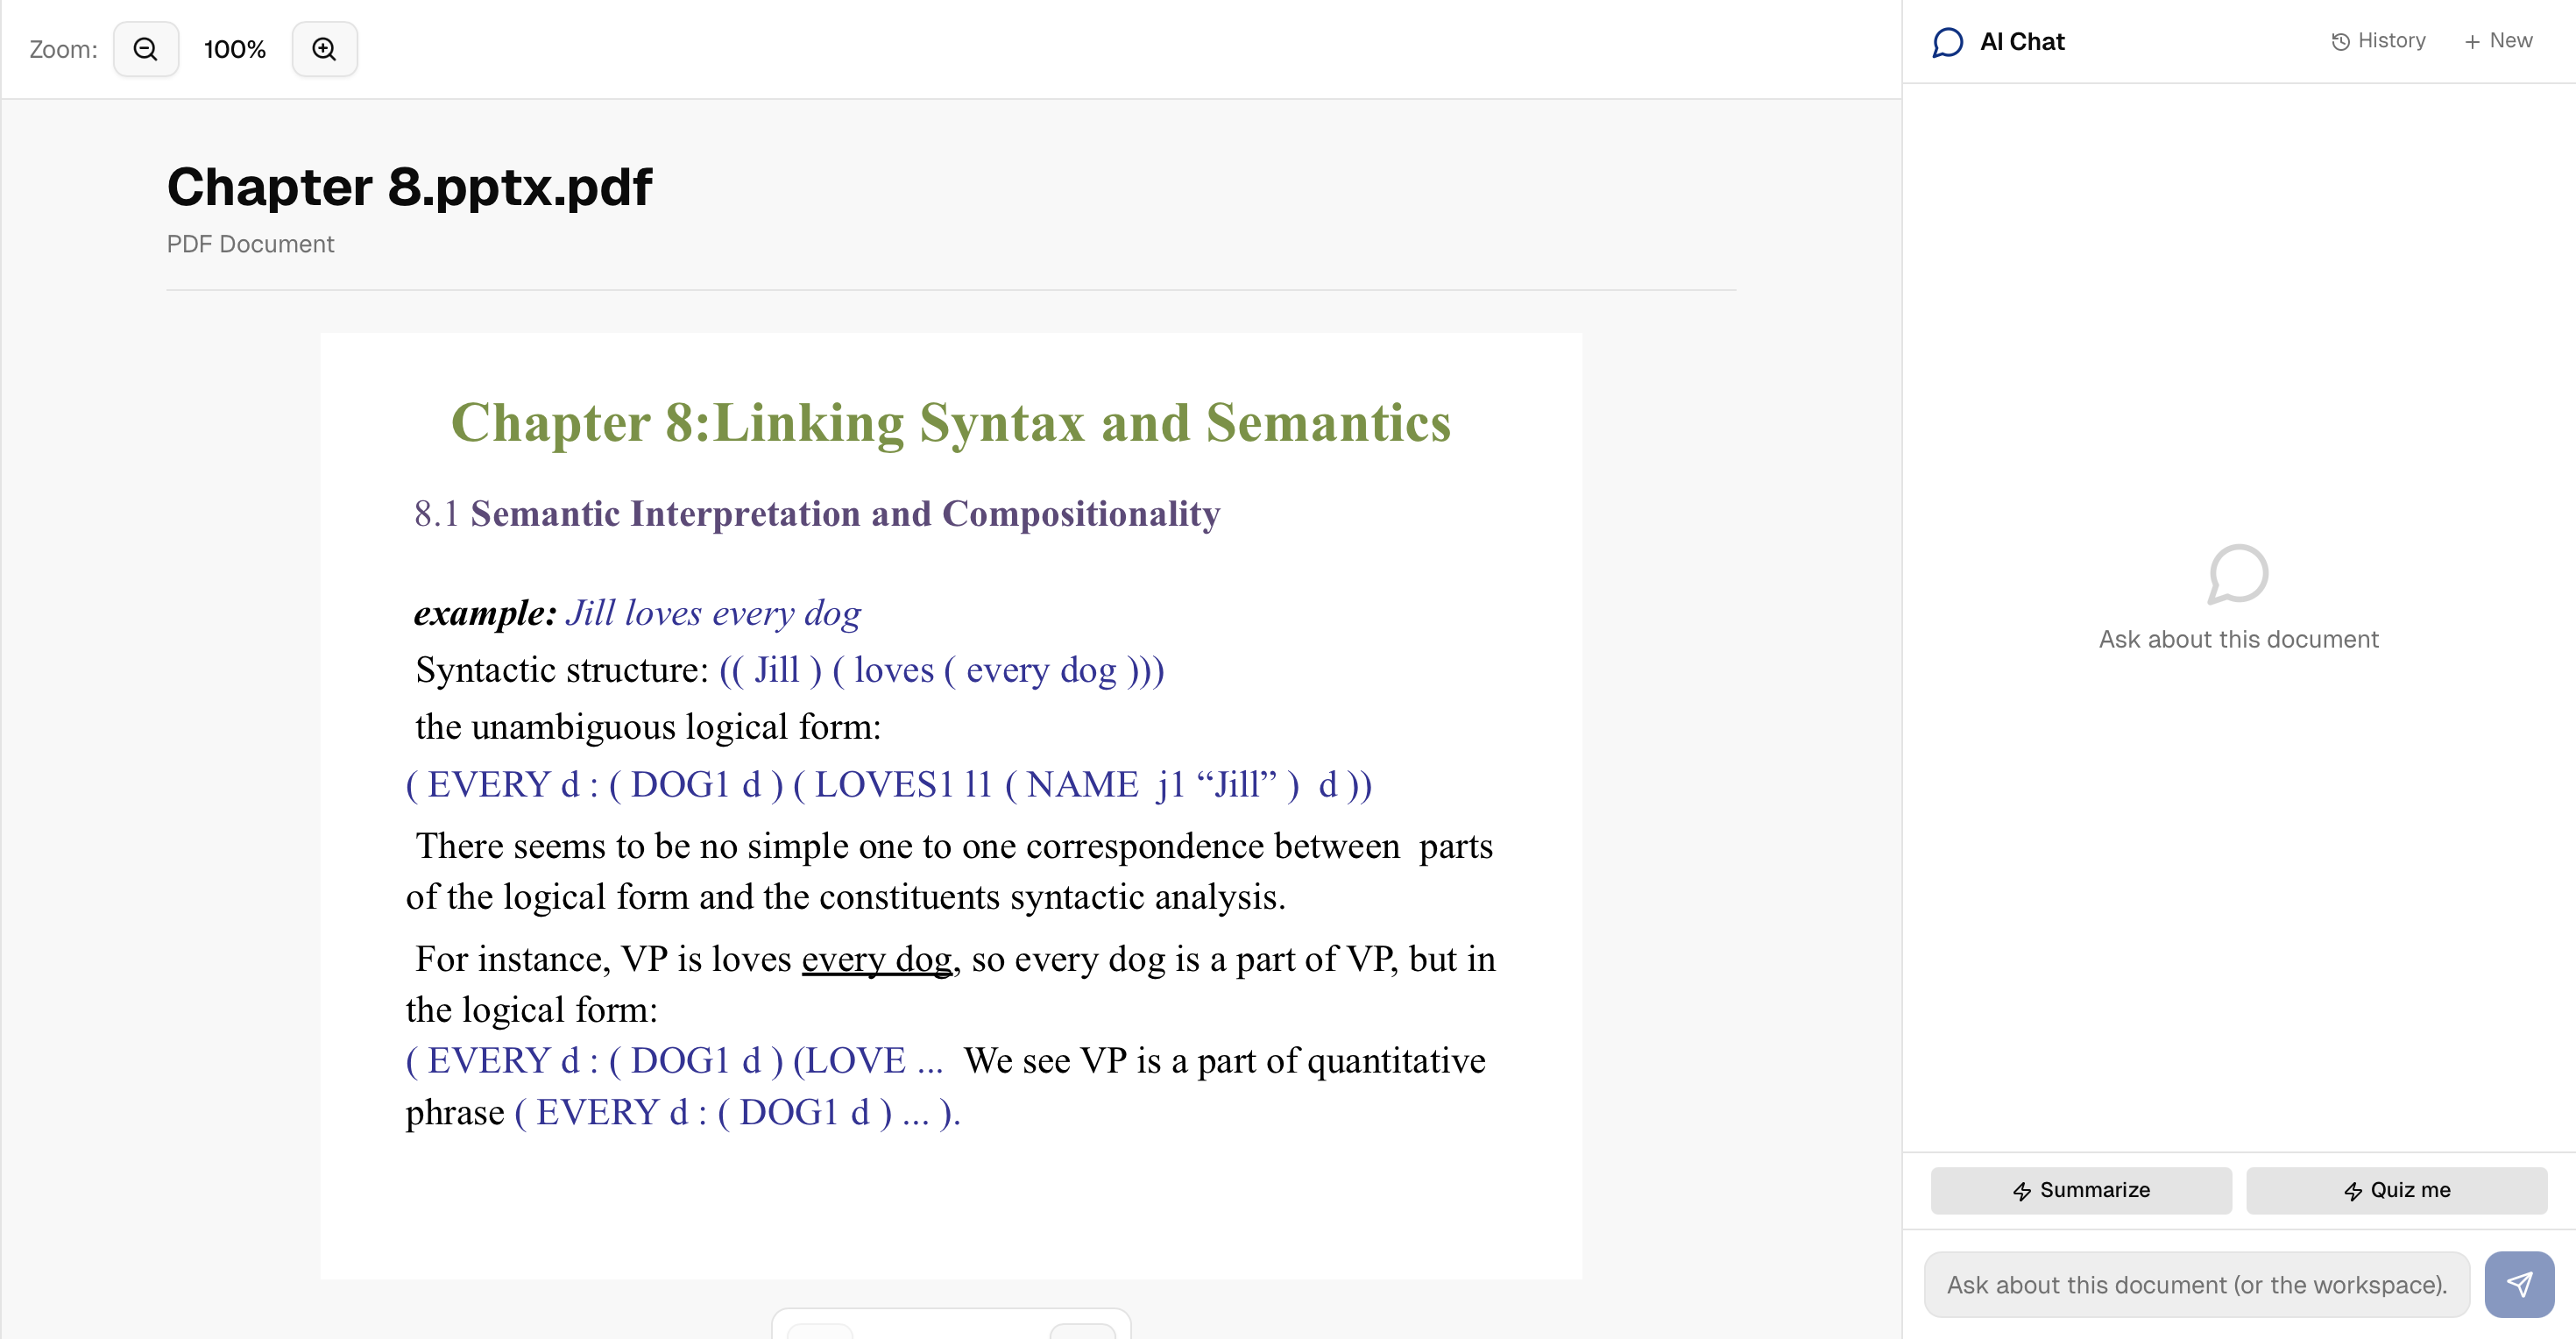
\includegraphics[width=0.92\linewidth]{images/ui-ux/split-screen.png}
\end{figure}

\begin{itemize}
    \item \textbf{Bên trái.} Trình xem tài liệu hiển thị nội dung PDF hoặc văn bản thô với các công cụ như phóng to, thu nhỏ và cuộn độc lập.
    \item \textbf{Bên phải.} Khung chat nơi người dùng đặt câu hỏi và nhận phản hồi kèm trích dẫn.
    \item \textbf{Mục tiêu sử dụng.} Giữ cho người dùng luôn làm việc trong cùng một ngữ cảnh mà không cần chuyển qua lại giữa nhiều cửa sổ.
\end{itemize}

\subsubsection{Cơ chế trích dẫn và liên kết ngược}
Khác biệt quan trọng của UX trong DigitalBookLLM là khả năng kết nối trực tiếp giữa câu trả lời của AI và tài liệu gốc.

\begin{figure}[H]
    \centering
    \caption{Cơ chế trích dẫn và làm nổi bật đoạn văn liên quan trong tài liệu}
    \label{fig:ui-citation}
    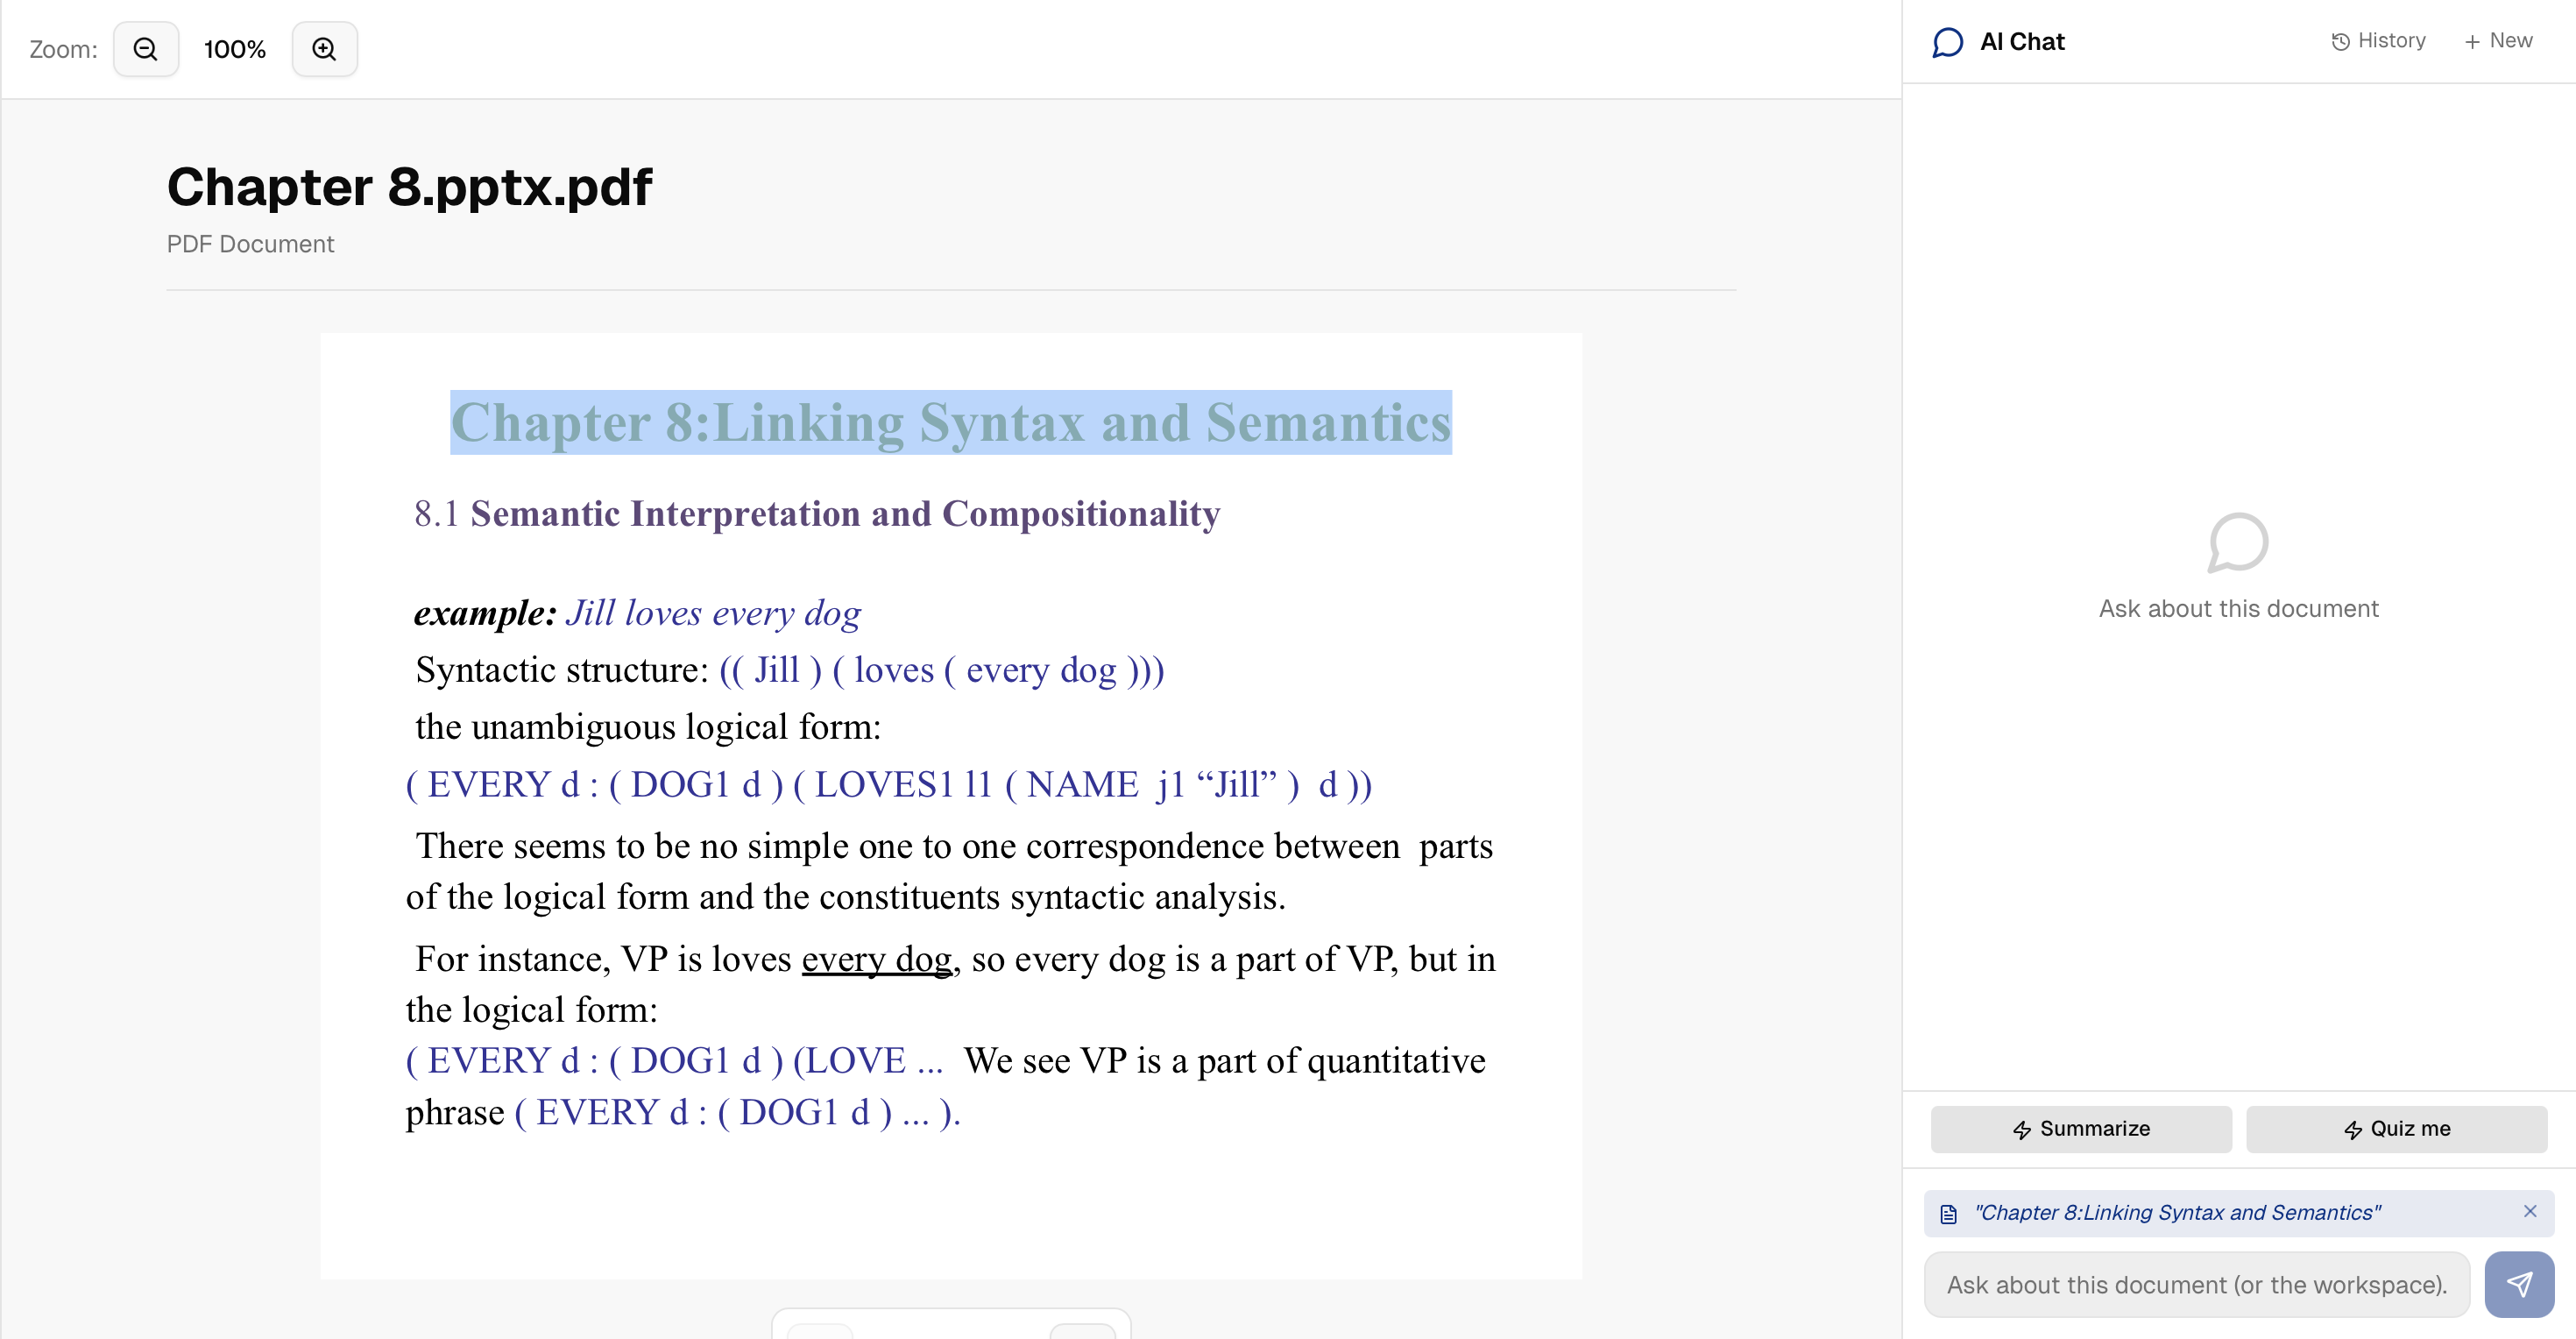
\includegraphics[width=0.92\linewidth]{images/ui-ux/highlight.png}
\end{figure}

\begin{itemize}
    \item \textbf{Cách thức hoạt động.} Các thẻ trích dẫn trong câu trả lời cho phép người dùng nhấp vào và tự động cuộn tài liệu sang vị trí liên quan.
    \item \textbf{Hiệu ứng trực quan.} Đoạn văn bản tương ứng được làm nổi bật để củng cố mối liên hệ giữa phản hồi và nguồn gốc tri thức.
    \item \textbf{Mục tiêu sử dụng.} Tăng độ tin cậy của phản hồi và hỗ trợ quá trình đối chiếu nội dung ngay trên tài liệu nguồn.
\end{itemize}

\subsubsection{Thanh công cụ ngữ cảnh nổi (Contextual Popover)}
Đây là điểm chạm giải quyết trực tiếp bài toán thao tác rườm rà đã nêu ở Chương 1: khi người dùng bôi đen một đoạn văn bản, một thanh công cụ nhỏ hiện ra ngay phía trên vùng chọn với bốn hành động (Highlight, Note, Speak, Ask AI), thay vì buộc người dùng phải mở một menu riêng hay chuyển đổi ứng dụng.

\begin{figure}[H]
    \centering
    
\includegraphics[width=0.92\linewidth]{images/ui-ux/selection-toolbar.png}
    \caption{Thanh công cụ ngữ cảnh hiển thị phía trên vùng văn bản được chọn}
    \label{fig:ui-selection-toolbar}
\end{figure}

\begin{itemize}
    \item \textbf{Highlight.} Mở một bảng chọn màu nhỏ; sau khi chọn, đoạn văn bản được tô màu và lưu lại vị trí (UC-11).
    \item \textbf{Note.} Mở một ô nhập văn bản ngắn để đính kèm ghi chú cá nhân vào đoạn đã chọn.
    \item \textbf{Speak.} Phát âm thanh đọc to đoạn văn bản theo thời gian thực (UC-12).
    \item \textbf{Ask AI.} Focus khung chat, chèn đoạn văn bản đã chọn vào dưới dạng thẻ trích dẫn kèm ba gợi ý câu hỏi nhanh (UC-14).
\end{itemize}

\subsubsection{Màn hình khám phá đồ thị tri thức (Knowledge Graph Explorer)}
Khi chuyển sang Graph Mode, canvas trung tâm hiển thị mạng lưới nút và cạnh biểu diễn các khái niệm người dùng đã tương tác qua nhiều tài liệu và phiên chat (UC-15). Nút được tô màu theo loại thực thể (khái niệm, nhân vật, công nghệ); nhấn vào một nút mở panel chi tiết bên phải, hiển thị mô tả và các đoạn trích dẫn nguồn liên quan.

% \textit{Ảnh chụp màn hình cho mục này chưa có sẵn trong bộ tài nguyên hình ảnh của đồ án; xem tệp theo dõi công việc còn lại để bổ sung.}

\subsection{Khả năng đáp ứng và ngôn ngữ giao diện}
Bố cục chia đôi chuyển thành xếp chồng (trình đọc phía trên, khung chat phía dưới) khi chiều rộng màn hình dưới 768px, với thanh bên (sidebar) thu gọn thành lớp phủ (overlay) trên thiết bị di động. Toàn bộ giao diện hỗ trợ song ngữ Việt/Anh với nút chuyển đổi ở thanh header, đi kèm chế độ sáng/tối/theo hệ thống (UC-09).

\chapter{Thiết kế kiến trúc hệ thống}

\textit{Chương 5 phân tích các quyết định kiến trúc cấu thành nên hệ thống DigitalBookLLM: kiến trúc modular monolith kết hợp async workers, ngăn xếp công nghệ, kỹ thuật RAG ưu tiên ngữ cảnh (hard-context), kiến trúc đồ thị tri thức cá nhân hóa, và các cơ chế bảo mật, hiệu năng.}

\section{Lựa chọn mô hình kiến trúc tổng quát}
Kiến trúc tổng quát của DigitalBookLLM được lựa chọn theo mô hình \textbf{modular monolith kết hợp async workers}: toàn bộ nghiệp vụ chạy trong một ứng dụng máy chủ duy nhất, được tổ chức thành các mô-đun dịch vụ tách biệt rõ ràng, trong khi các tác vụ nặng (xử lý tài liệu, trích xuất tri thức) được đẩy sang một hàng đợi xử lý bất đồng bộ thay vì chạy đồng bộ trên luồng xử lý yêu cầu chính.

\subsection{Kiến trúc client-server}
Hệ thống được tổ chức thành hai tầng logic tách biệt, giao tiếp qua HTTP/REST và Server-Sent Events (SSE):

\begin{description}[style=nextline, leftmargin=3.5em, labelsep=0.6em]
    \item[\textbf{Tầng giao diện (Client)}] Ứng dụng Next.js chạy trên trình duyệt, chịu trách nhiệm hiển thị màn hình chia đôi, gửi yêu cầu REST cho các thao tác CRUD, và tiêu thụ luồng SSE cho phản hồi AI theo thời gian thực.
    \item[\textbf{Tầng máy chủ (Server)}] Ứng dụng Express (Node.js) xử lý xác thực, quản lý tài liệu/highlight/đồ thị tri thức, điều phối pipeline RAG, và vận hành hàng đợi tác vụ nền, tất cả trong cùng một tiến trình triển khai.
\end{description}

\subsection{Xử lý bất đồng bộ qua hàng đợi tác vụ}
Các tác vụ tốn thời gian, như trích xuất văn bản, OCR, phân đoạn, nhúng vector, trích xuất thực thể cho đồ thị tri thức, không chạy trực tiếp trong vòng đời một yêu cầu HTTP. Khi người dùng tải tài liệu lên, máy chủ lưu tệp, tạo bản ghi với trạng thái \texttt{UPLOADED}, đưa một tác vụ vào hàng đợi, và trả về ngay mã \texttt{202 Accepted}. Một nhóm worker với số lượng đồng thời giới hạn liên tục giành và xử lý các tác vụ đang chờ, cập nhật trạng thái tài liệu khi hoàn tất. Cách tổ chức này tách rời hoàn toàn luồng phản hồi giao diện khỏi khối lượng công việc xử lý AI, đáp ứng trực tiếp yêu cầu NFR-02.2.

\subsection{Nguyên tắc cô lập dữ liệu đa người dùng}
Vì hệ thống phục vụ nhiều người dùng đồng thời trên cùng một hạ tầng dùng chung, mọi bảng dữ liệu và mọi đường truy vấn đều mang và lọc theo định danh người dùng (\texttt{user\_id}). Đây không phải một lớp bảo vệ tập trung duy nhất, mà là một nguyên tắc được áp dụng nhất quán ở từng dịch vụ truy xuất dữ liệu. Cách tiếp cận này được kiểm chứng trực tiếp bằng bộ kiểm thử chống truy cập trái phép (IDOR) ở Chương 6.


\section{Lựa chọn các thành phần công nghệ (Technology Stack)}
Để hiện thực hóa DigitalBookLLM, nhóm lựa chọn một tập hợp công nghệ hiện đại, ưu tiên các nền tảng có gói triển khai miễn phí để đáp ứng yêu cầu công khai hệ thống trong phạm vi ngân sách của một đồ án.

\subsection{Tầng trình diễn: Next.js và Tailwind CSS}
\begin{description}
    \item[\textbf{Next.js}] Hỗ trợ tốt cho quản lý trạng thái phức tạp, điều hướng ứng dụng và khả năng kết xuất linh hoạt; phù hợp với yêu cầu duy trì đồng thời trình xem tài liệu và khung chat trên một màn hình chia đôi.
    \item[\textbf{Tailwind CSS}] Cho phép xây dựng giao diện theo hướng tiện ích (utility-first), giúp kiểm soát nhanh bố cục phản hồi, khoảng cách và tính nhất quán trên nhiều kích thước màn hình.
\end{description}

\subsection{Tầng máy chủ: Node.js và Express}
\begin{itemize}
    \item \textbf{Kiến trúc hướng sự kiện.} Node.js phù hợp với khối lượng công việc gần như hoàn toàn phụ thuộc vào I/O mạng (gọi LLM, truy vấn cơ sở dữ liệu, lưu trữ đối tượng), tương đương về thông lượng với các framework bất đồng bộ khác cho cùng dạng tải.
    \item \textbf{Hỗ trợ streaming.} Express giúp triển khai đơn giản các tuyến API phục vụ truyền phản hồi theo luồng (SSE) từ mô hình ngôn ngữ đến giao diện.
    \item \textbf{Hệ kiểu dùng chung.} Việc dùng TypeScript ở cả client lẫn server loại bỏ sự trùng lặp định nghĩa kiểu dữ liệu giữa hai phía.
\end{itemize}

\subsection{Hệ quản trị dữ liệu: PostgreSQL và phần mở rộng \texttt{pgvector}}
\begin{itemize}
    \item \textbf{PostgreSQL} đảm nhiệm lưu trữ dữ liệu quan hệ: người dùng, không gian làm việc, tài liệu, highlight, phiên hội thoại và hàng đợi tác vụ.
    \item \textbf{\texttt{pgvector}} bổ sung khả năng lập chỉ mục HNSW và truy vấn tương đồng vector ngay trong cùng hệ quản trị cơ sở dữ liệu, loại bỏ nhu cầu một kho vector chuyên dụng riêng biệt.
    \item \textbf{Lưu trữ đối tượng.} Tệp tài liệu gốc và ảnh bìa được lưu ở một dịch vụ lưu trữ đối tượng tương thích S3, tách biệt khỏi cơ sở dữ liệu quan hệ.
\end{itemize}

\subsection{Bộ định tuyến LLM đa nhà cung cấp}
Vì các dịch vụ LLM ở gói miễn phí không cam kết tính khả dụng liên tục, tầng AI của hệ thống không gọi trực tiếp một nhà cung cấp cố định mà thông qua một bộ định tuyến (LLM Router) có khả năng tự dò trạng thái và chuyển đổi:

\begin{itemize}
    \item \textbf{Mô hình nhúng cục bộ} (\texttt{all-MiniLM-L6-v2}, 384 chiều) chạy trên CPU của máy chủ, không phụ thuộc hạn mức của bất kỳ API bên ngoài nào cho bước truy xuất; chỉ bước sinh câu trả lời mới cần gọi LLM.
    \item \textbf{Thứ tự ưu tiên ba tầng:} (1) các nhà cung cấp do người vận hành cấu hình (theo thứ tự khai báo trong biến môi trường); (2) Google Gemini (gói miễn phí, hạn mức rộng); (3) Groq (thời gian phản hồi thấp, dùng làm phương án cuối).
    \item \textbf{Dò trạng thái khả dụng (health check)} cho từng nhà cung cấp bằng một yêu cầu thăm dò nhẹ, kết quả được lưu đệm 30 giây để tránh dò lại liên tục; nhà cung cấp chưa cấu hình hoặc không khả dụng bị bỏ qua trước khi định tuyến.
    \item \textbf{Chuyển đổi khi lỗi (failover):} nếu nhà cung cấp được chọn báo lỗi trước khi trả về bất kỳ dữ liệu nào, bộ định tuyến tự động thử nhà cung cấp kế tiếp trong danh sách mà không để lộ lỗi ra phía người dùng.
    \item \textbf{Hàng đợi tác vụ bền vững} lưu trong chính PostgreSQL, xử lý song song có giới hạn, thay thế vai trò một message broker chuyên dụng.
\end{itemize}


\section{Kiến trúc RAG ưu tiên ngữ cảnh (Prioritized RAG)}
Thay vì để mô hình tự tìm lại ngữ cảnh bằng tìm kiếm vector trong mọi trường hợp, DigitalBookLLM phân biệt rõ hai chế độ hỏi đáp dựa trên việc người dùng có chọn sẵn một đoạn văn bản hay không, và luôn ưu tiên tuyệt đối đoạn văn bản đó khi nó tồn tại.

\subsection{Hai chế độ truy xuất}
\begin{description}
    \item[\textbf{Hỏi đáp toàn cục (UC-13)}] Không có đoạn văn bản nào được chọn. Câu hỏi được nhúng thành vector và tìm kiếm tương đồng trên tài liệu đang mở; nếu độ tương đồng cao nhất dưới một ngưỡng cấu hình, hệ thống mở rộng phạm vi tìm kiếm ra toàn bộ không gian làm việc.
    \item[\textbf{Hỏi đáp theo ngữ cảnh (UC-14)}] Người dùng đã chọn một đoạn văn bản cụ thể. Đoạn văn bản này được đưa vào lời nhắc dưới dạng \textit{ngữ cảnh cứng} (hard context): bắt buộc, không thể bị loại bỏ bởi kết quả tìm kiếm vector, đúng theo yêu cầu FR-07. Kết quả tìm kiếm vector (nếu có) chỉ đóng vai trò bổ sung.
\end{description}

\subsection{Luồng xử lý một yêu cầu hỏi đáp}
\begin{enumerate}
    \item Truy xuất các phân đoạn liên quan (nếu cần) và gửi ngay danh sách trích dẫn về giao diện qua SSE, trước cả khi mô hình ngôn ngữ bắt đầu sinh câu trả lời. Nhờ vậy trích dẫn luôn hiển thị được kể cả khi bước sinh câu trả lời gặp sự cố.
    \item Xây dựng lời nhắc gồm: chỉ dẫn hệ thống, ngữ cảnh cứng (nếu có), các phân đoạn truy xuất được, và lịch sử hội thoại gần nhất của phiên.
    \item Gửi lời nhắc đến bộ định tuyến LLM (mục 5.2), nhận phản hồi dạng luồng và chuyển tiếp từng token về giao diện qua SSE.
    \item Lưu cặp câu hỏi--trả lời cùng danh sách trích dẫn vào lịch sử phiên, đồng thời đưa một tác vụ trích xuất tri thức vào hàng đợi để cập nhật đồ thị tri thức cá nhân (mục 5.4).
\end{enumerate}

\subsection{Giới hạn được ghi nhận}
Cách tiếp cận này không giải quyết truy vấn đa bước (multi-hop) đòi hỏi đối chiếu thông tin giữa nhiều tài liệu hoặc nhiều chương khác nhau trong một lượt truy xuất duy nhất. Đây là giới hạn đã nêu ở Chương 1, được ghi nhận là hướng phát triển tiếp theo ở Chương 7, thay vì được giải quyết bằng một kiến trúc tác tử đa bước trong phạm vi đồ án này (NFR-03.2).


\section{Kiến trúc đồ thị tri thức cá nhân hóa}
Song song với pipeline RAG, DigitalBookLLM vận hành một pipeline thứ hai chạy hoàn toàn ở chế độ nền: trích xuất thực thể và quan hệ từ nội dung người dùng đã tương tác, tích lũy dần thành một đồ thị tri thức cá nhân cho từng tài khoản (FR-06, UC-15).

\subsection{Nguyên tắc thiết kế: không chặn trải nghiệm chính}
Trích xuất tri thức không bao giờ nằm trên đường xử lý của một yêu cầu đọc hoặc hỏi đáp. Sau mỗi lượt hỏi đáp AI thành công, hoặc sau khi một tài liệu được nạp xong, hệ thống chỉ đơn giản đưa thêm một tác vụ \texttt{EXTRACT\_ENTITIES} vào hàng đợi chung đã mô tả ở mục 5.1, rồi trả lời ngay cho người dùng. Việc đồ thị được cập nhật muộn vài giây sau không ảnh hưởng đến trải nghiệm đọc và hỏi đáp.

\subsection{Trích xuất thực thể và quan hệ}
Worker xử lý tác vụ gửi đoạn văn bản liên quan (đoạn được chọn, câu hỏi và câu trả lời, hoặc toàn văn tài liệu khi mới nạp xong) đến bộ định tuyến LLM, yêu cầu trả về trực tiếp một cấu trúc dữ liệu gồm danh sách thực thể (tên, loại, mô tả) và danh sách quan hệ (thực thể nguồn, thực thể đích, loại quan hệ). Kết quả được hợp nhất (upsert) vào đồ thị của người dùng: thực thể trùng tên được cập nhật mô tả thay vì tạo bản sao; quan hệ mới được thêm cùng tài liệu nguồn và đoạn trích minh chứng để phục vụ tra cứu ngược.

\subsection{Lưu trữ đồ thị trong PostgreSQL (ADR-04)}
Đồ thị được lưu bằng hai bảng quan hệ, \texttt{entities} (nút) và \texttt{entity\_relations} (cạnh), thay vì một hệ quản trị đồ thị chuyên dụng. Quyết định này dựa trên hai lý do:
\begin{itemize}
    \item \textbf{Quy mô truy vấn thực tế nhỏ.} Giao diện khám phá chỉ cần truy vấn lân cận một hoặc hai bước quanh một nút được chọn (xem Chương 2, mục Knowledge Graph). Một truy vấn đệ quy (recursive CTE) trên PostgreSQL phục vụ tốt ở quy mô một đồ thị cá nhân (vài trăm đến vài nghìn nút).
    \item \textbf{Nhất quán vận hành.} Lưu đồ thị cùng cơ sở dữ liệu quan hệ chính giúp việc cô lập dữ liệu theo người dùng (NFR-04.1) và xóa tuần tự khi tài khoản/tài liệu bị xóa dùng chung một cơ chế với mọi bảng khác, thay vì phải đồng bộ hai hệ lưu trữ riêng biệt.
\end{itemize}

\subsection{Truy vấn phục vụ giao diện khám phá}
Điểm cuối \texttt{GET /api/graph} trả về toàn bộ nút và cạnh thuộc về người dùng hiện tại để dựng mạng lưới nút và cạnh trên giao diện. Điểm cuối \texttt{GET /api/graph/:entityId} trả về chi tiết một nút cùng danh sách nút lân cận và đoạn trích nguồn, phục vụ panel chi tiết khi người dùng nhấn vào một nút trong đồ thị.


\section{Kiến trúc bảo mật và hiệu năng hệ thống}

\subsection{Cô lập dữ liệu và chống truy cập trái phép (IDOR)}
Vì hệ thống phục vụ nhiều người dùng trên cùng một hạ tầng dùng chung, biện pháp bảo mật quan trọng nhất là ngăn chặn IDOR: tình trạng một người dùng truy vấn được tài nguyên (tài liệu, highlight, đồ thị tri thức) của người dùng khác chỉ bằng cách đoán hoặc biết được định danh (NFR-04.1).

\begin{itemize}
    \item \textbf{Kiểm tra quyền sở hữu tại tầng dịch vụ.} Mọi phương thức truy vấn dữ liệu ở tầng dịch vụ (không phải chỉ ở tầng controller) đều nhận vào và lọc theo \texttt{userId} rút ra từ token JWT đã xác thực, không bao giờ tin vào định danh do client tự khai trong tham số truy vấn.
    \item \textbf{Xác thực không trạng thái.} Token JWT có thời hạn (mặc định 7 ngày), được xác minh ở một middleware duy nhất áp dụng cho toàn bộ các tuyến API cần xác thực.
    \item \textbf{Kiểm chứng bằng kiểm thử tự động.} Bộ kiểm thử bảo mật (Chương 6) mô phỏng người dùng B cố truy cập tài nguyên của người dùng A qua workspace, tài liệu và highlight, xác minh mọi trường hợp đều trả về 403/404.
\end{itemize}

\subsection{Kiểm soát tải và giới hạn tần suất}
\begin{itemize}
    \item \textbf{Giới hạn tần suất theo danh tính.} Thay vì giới hạn theo địa chỉ IP, hệ thống áp dụng hạn mức truy vấn AI theo từng tài khoản mỗi ngày, vì giới hạn theo IP dễ bị vô hiệu hóa (nhiều người dùng sau cùng một NAT) hoặc gây bất công (nhiều tài khoản sau cùng một IP).
    \item \textbf{Hàng đợi tác vụ có giới hạn đồng thời.} Số lượng worker xử lý song song được giới hạn cấu hình; khi số tác vụ vượt quá khả năng xử lý tức thời, chúng xếp hàng trong bảng \texttt{jobs} thay vì làm sập tiến trình máy chủ API (NFR-02.2).
    \item \textbf{Thử lại có độ trễ tăng dần.} Tác vụ lỗi được thử lại tối đa 3 lần với thời gian chờ tăng dần theo cấp số nhân, sau đó chuyển sang trạng thái \texttt{DEAD} kèm thông tin lỗi thay vì lặp vô hạn.
\end{itemize}

\subsection{Khả dụng của tầng AI}
Vì hệ thống phụ thuộc vào các nhà cung cấp LLM bên thứ ba ở gói miễn phí, tính khả dụng của tầng AI được xử lý bằng cơ chế dò trạng thái và chuyển đổi nhà cung cấp đã trình bày ở mục 5.2, thay vì giả định một nhà cung cấp duy nhất luôn sẵn sàng. Khi toàn bộ nhà cung cấp đều không khả dụng, hệ thống trả về một sự kiện lỗi rõ ràng qua luồng SSE thay vì để yêu cầu treo hoặc trả lỗi 500 chung chung.

\subsection*{Tổng kết Chương 5}
Chương này đã trình bày kiến trúc modular monolith kết hợp async workers của DigitalBookLLM, ngăn xếp công nghệ được lựa chọn theo tiêu chí chi phí triển khai và tính khả dụng, cơ chế RAG ưu tiên ngữ cảnh cứng, kiến trúc đồ thị tri thức cá nhân hoá lưu trữ quan hệ, cùng các biện pháp bảo mật và kiểm soát tải. Các quyết định thay thế cụ thể so với kiến trúc tham chiếu ban đầu (ví dụ thay RabbitMQ/Celery bằng hàng đợi PostgreSQL, thay Neo4j bằng lưu trữ quan hệ) cùng lý do được ghi nhận đầy đủ trong tài liệu kiến trúc đính kèm đồ án.


\chapter{Hiện thực và Đánh giá Hệ thống}

\textit{Chương 6 trình bày kết quả hiện thực của hệ thống và kế hoạch kiểm thử được xây dựng để đánh giá hệ thống theo từng nhóm use case và yêu cầu phi chức năng, cùng kết quả thực thi thực tế.}

\section{Kết quả hiện thực}
Toàn bộ kiến trúc trình bày ở Chương 5 đã được hiện thực đầy đủ: ứng dụng web Next.js, máy chủ API Express với hàng đợi tác vụ nền, pipeline nạp tài liệu (trích xuất văn bản, OCR dự phòng, phân đoạn hai bước, nhúng vector), pipeline hỏi đáp RAG ưu tiên ngữ cảnh cứng với truyền phản hồi dạng luồng, bộ định tuyến LLM đa nhà cung cấp, và pipeline trích xuất tri thức xây dựng đồ thị cá nhân hoá chạy nền.

Hệ thống được đóng gói bằng Docker cho cả máy chủ API lẫn ứng dụng web, triển khai được đồng thời trên một máy cục bộ (\texttt{docker compose up}) lẫn trên các nền tảng có gói miễn phí công khai. Toàn bộ 15 trường hợp sử dụng đặc tả ở Chương 3 đều đã được hiện thực và kiểm thử ở mức độ tương ứng với NFR-03.1/NFR-03.2 (chấp nhận sai số OCR, không tích hợp tác tử phức tạp).

\section{Môi trường kiểm thử}
Kết quả trình bày trong chương này được ghi nhận từ một môi trường container hóa cục bộ, mô phỏng sát điều kiện triển khai công khai:
\begin{itemize}
    \item PostgreSQL 16 với phần mở rộng \texttt{pgvector} (chỉ mục HNSW), chạy trong container riêng.
    \item Máy chủ API chạy trong container Debian-slim (cần thiết cho các phụ thuộc gốc của module dựng ảnh PDF và OCR).
    \item Không cấu hình khóa API cho nhà cung cấp LLM nào trong môi trường đo, nên các kết quả về truy xuất (retrieval) độc lập với tính khả dụng của dịch vụ AI bên thứ ba; kết quả về sinh câu trả lời (generation) được ghi chú riêng là "không áp dụng" khi không có nhà cung cấp nào khả dụng.
\end{itemize}


\section{Kế hoạch kiểm thử}
Kế hoạch kiểm thử được tổ chức thành năm nhóm, tương ứng với năm nhóm use case và các yêu cầu phi chức năng trọng tâm. Bảng dưới đây trình bày các kịch bản đại diện của mỗi nhóm; bộ kịch bản đầy đủ và kết quả thực thi chi tiết được trình bày ở Phụ lục A.

\subsection{Nhóm kiểm thử: Tài liệu và xử lý nền}
\textit{Mục tiêu:} Đảm bảo hệ thống tải file thành công và worker xử lý ngầm (OCR, phân đoạn, nhúng vector) chạy chính xác.

\begin{longtable}{|C{0.08\textwidth}|C{0.12\textwidth}|L{0.30\textwidth}|L{0.42\textwidth}|}
\caption{Kịch bản kiểm thử đại diện: Tài liệu và xử lý nền}\\
\hline
\textbf{Mã TC} & \textbf{UC/FR} & \textbf{Kịch bản} & \textbf{Kết quả mong đợi} \\\hline
\endfirsthead
\hline
\textbf{Mã TC} & \textbf{UC/FR} & \textbf{Kịch bản} & \textbf{Kết quả mong đợi} \\\hline
\endhead
TC-DOC-01 & UC-05, FR-03 & Tải lên tài liệu PDF có lớp văn bản & Trạng thái chuyển \texttt{UPLOADED} $\to$ \texttt{READY}; tệp gốc lưu vào kho đối tượng. \\\hline
TC-DOC-02 & UC-07, FR-04 & Theo dõi tiến trình worker xử lý ngầm & Phân đoạn, vector được lưu; trạng thái tài liệu chuyển đúng thứ tự. \\\hline
TC-DOC-03 & UC-07, NFR-03.1 & Xử lý OCR cho PDF dạng ảnh quét & Worker gọi OCR thành công; chấp nhận một tỉ lệ sai số nhận diện. \\\hline
\end{longtable}

\subsection{Nhóm kiểm thử: Trải nghiệm đọc sách}
\textit{Mục tiêu:} Đảm bảo giao diện mượt mà, render tối ưu và tương tác theo ngữ cảnh hoạt động đúng.

\begin{longtable}{|C{0.08\textwidth}|C{0.12\textwidth}|L{0.30\textwidth}|L{0.42\textwidth}|}
\caption{Kịch bản kiểm thử đại diện: Trải nghiệm đọc sách}\\
\hline
\textbf{Mã TC} & \textbf{UC/FR} & \textbf{Kịch bản} & \textbf{Kết quả mong đợi} \\\hline
\endfirsthead
\hline
\textbf{Mã TC} & \textbf{UC/FR} & \textbf{Kịch bản} & \textbf{Kết quả mong đợi} \\\hline
\endhead
TC-READ-01 & UC-08, FR-08 & Mở tài liệu PDF trên 1500 trang, cuộn nhanh & Thời gian mở dưới 3 giây; trình duyệt không treo. \\\hline
TC-READ-02 & UC-11 & Bôi đen văn bản hiện thanh công cụ nổi & Popover với 4 hành động hiện ngay phía trên vùng chọn. \\\hline
TC-READ-03 & UC-11 & Thêm highlight, tải lại trang & Đoạn văn được tô đúng màu, đúng vị trí sau khi tải lại. \\\hline
\end{longtable}

\subsection{Nhóm kiểm thử: Tương tác AI và RAG}
\textit{Mục tiêu:} Xác minh AI lấy đúng ngữ cảnh, không ảo giác, và truyền phản hồi mượt mà.

\begin{longtable}{|C{0.08\textwidth}|C{0.12\textwidth}|L{0.30\textwidth}|L{0.42\textwidth}|}
\caption{Kịch bản kiểm thử đại diện: Tương tác AI và RAG}\\
\hline
\textbf{Mã TC} & \textbf{UC/FR} & \textbf{Kịch bản} & \textbf{Kết quả mong đợi} \\\hline
\endfirsthead
\hline
\textbf{Mã TC} & \textbf{UC/FR} & \textbf{Kịch bản} & \textbf{Kết quả mong đợi} \\\hline
\endhead
TC-AI-01 & UC-14, FR-07 & Hỏi đáp theo ngữ cảnh đã chọn & Câu trả lời bám sát đúng đoạn văn bản đã chọn. \\\hline
TC-AI-02 & NFR-02.1 & Đo độ trễ truyền dữ liệu AI & TTFB dưới 2 giây; dữ liệu trả về dạng luồng SSE. \\\hline
TC-AI-03 & UC-13 & Nhấn vào thẻ trích dẫn & Trình đọc tự động cuộn đến đúng trang chứa ngữ cảnh. \\\hline
\end{longtable}

\subsection{Nhóm kiểm thử: Cá nhân hoá (Knowledge Graph)}
\textit{Mục tiêu:} Đảm bảo đồ thị tri thức tiến hoá đúng dựa trên tương tác của người dùng.

\begin{longtable}{|C{0.08\textwidth}|C{0.12\textwidth}|L{0.30\textwidth}|L{0.42\textwidth}|}
\caption{Kịch bản kiểm thử đại diện: Cá nhân hoá}\\
\hline
\textbf{Mã TC} & \textbf{UC/FR} & \textbf{Kịch bản} & \textbf{Kết quả mong đợi} \\\hline
\endfirsthead
\hline
\textbf{Mã TC} & \textbf{UC/FR} & \textbf{Kịch bản} & \textbf{Kết quả mong đợi} \\\hline
\endhead
TC-KG-01 & UC-15, FR-06 & Tự động sinh đồ thị từ hội thoại & Node mới xuất hiện đúng, gán đúng \texttt{user\_id}. \\\hline
TC-KG-02 & FR-06 & Trích xuất tri thức không chặn phản hồi chat & Phản hồi chat trả về bình thường dù worker trích xuất đang chạy. \\\hline
\end{longtable}

\subsection{Nhóm kiểm thử: Bảo mật và Hiệu năng}
\textit{Mục tiêu:} Đảm bảo kiến trúc an toàn, bảo vệ dữ liệu và chịu tải tốt.

\begin{longtable}{|C{0.08\textwidth}|C{0.12\textwidth}|L{0.30\textwidth}|L{0.42\textwidth}|}
\caption{Kịch bản kiểm thử đại diện: Bảo mật và Hiệu năng}\\
\hline
\textbf{Mã TC} & \textbf{UC/FR} & \textbf{Kịch bản} & \textbf{Kết quả mong đợi} \\\hline
\endfirsthead
\hline
\textbf{Mã TC} & \textbf{UC/FR} & \textbf{Kịch bản} & \textbf{Kết quả mong đợi} \\\hline
\endhead
TC-SEC-01 & FR-01, NFR-04.1 & Người dùng B truy cập tài nguyên của A bằng UUID & Hệ thống từ chối, trả về 403/404. \\\hline
TC-PERF-01 & NFR-02.2 & 5--10 yêu cầu tải tài liệu đồng thời & API không sập; hàng đợi xử lý tuần tự, không mất tác vụ. \\\hline
\end{longtable}

\section{Kết quả kiểm thử}
Toàn bộ 28 kiểm thử đơn vị/tích hợp (Jest/Supertest), 6 kịch bản dò bảo mật IDOR, và các kiểm thử hiệu năng/RAG đại diện đều đạt kết quả \textbf{Pass}, chạy trên môi trường container hoá mô tả ở mục 6.2. Chi tiết từng kết quả, bao gồm số liệu đo được (thời gian phản hồi, tỉ lệ chấp nhận, recall@k), được trình bày đầy đủ ở Phụ lục A.


\chapter{Tổng kết}

\section{Tổng kết kết quả đạt được}
DigitalBookLLM đã hiện thực hóa được mục tiêu xây dựng một ứng dụng đọc sách điện tử tích hợp trợ lý AI trong cùng một không gian làm việc. Hệ thống hỗ trợ tải và đọc tài liệu đa định dạng, phân đoạn và lập chỉ mục vector, hỏi đáp theo ngữ cảnh toàn cục lẫn ngữ cảnh cứng (đoạn văn bản được chọn), trích dẫn trỏ ngược về đúng vị trí nguồn, đánh dấu/ghi chú tài liệu, phát âm thanh dạng luồng, và xây dựng đồ thị tri thức cá nhân từ lịch sử đọc và trò chuyện. Về mặt kiến trúc, dự án đã hình thành một chuỗi xử lý hoàn chỉnh từ tài liệu đầu vào đến phản hồi có căn cứ trên nguồn, vận hành ổn định cho nhiều người dùng đồng thời trên hạ tầng triển khai công khai miễn phí. Những kết quả này bám sát nền tảng lý thuyết về LLM, RAG, cơ sở dữ liệu vector và đồ thị tri thức đã trình bày ở Chương 2. \cite{lewis2020retrieval,gao2023retrieval,malkov2018efficient}

\section{Ưu điểm của hệ thống}
\begin{itemize}
    \item \textbf{Câu trả lời bám sát ngữ cảnh và có thể kiểm chứng.} Cơ chế ngữ cảnh cứng kết hợp trích dẫn trỏ ngược giúp phản hồi có căn cứ rõ ràng, giảm hiện tượng ảo giác và tăng khả năng kiểm chứng nội dung.
    \item \textbf{Trải nghiệm đọc và hỏi đáp hợp nhất.} Không gian làm việc chia đôi cùng thanh công cụ ngữ cảnh nổi (popover) loại bỏ thao tác sao chép thủ công giữa các ứng dụng.
    \item \textbf{Cá nhân hoá qua đồ thị tri thức.} Đồ thị tiến hoá tự động theo thời gian, cho phép người dùng nhìn lại quá trình học tập của bản thân qua nhiều tài liệu.
    \item \textbf{Kiến trúc rõ ràng và tiết kiệm chi phí vận hành.} Việc tách lớp dịch vụ và ưu tiên các nền tảng triển khai miễn phí cho phép hệ thống hoạt động công khai mà không cần ngân sách hạ tầng.
    \item \textbf{Khả năng phục hồi khi phụ thuộc bên ngoài gặp sự cố.} Bộ định tuyến LLM đa nhà cung cấp và hàng đợi tác vụ bền vững giúp hệ thống tiếp tục hoạt động (ở mức suy giảm) ngay cả khi một nhà cung cấp AI hoặc một lượt xử lý gặp lỗi tạm thời.
\end{itemize}

\section{Hạn chế của hệ thống}
\begin{itemize}
    \item \textbf{Chưa xử lý truy vấn đa bước (multi-hop).} Hệ thống chưa hỗ trợ câu hỏi đòi hỏi đối chiếu thông tin giữa nhiều tài liệu hoặc nhiều chương trong một lượt truy xuất duy nhất, do phạm vi đồ án giới hạn ở RAG một lượt (NFR-03.2).
    \item \textbf{Phụ thuộc vào tính khả dụng của nhà cung cấp LLM miễn phí.} Dù có cơ chế chuyển đổi tự động, chất lượng và tốc độ phản hồi vẫn phụ thuộc vào nhà cung cấp đang khả dụng tại thời điểm truy vấn.
    \item \textbf{Độ chính xác OCR còn giới hạn.} Đối với tài liệu quét chất lượng thấp, luồng OCR cơ bản có thể bỏ sót hoặc nhận diện sai một số ký tự (NFR-03.1).
    \item \textbf{Chưa hỗ trợ đăng nhập liên kết (OAuth).} Phiên bản hiện tại chỉ hỗ trợ email/mật khẩu.
    \item \textbf{Chưa có đánh giá tải ở quy mô lớn.} Các phép đo hiệu năng trong đồ án được thực hiện ở quy mô kiểm thử; cần thêm các đợt đánh giá với lượng người dùng đồng thời lớn hơn để kiểm chứng toàn diện hơn.
\end{itemize}

\section{Hướng phát triển}
\begin{itemize}
    \item \textbf{Truy vấn đa bước.} Bổ sung một lớp lập kế hoạch truy vấn con cho các câu hỏi đối chiếu nhiều tài liệu, mà không nhất thiết phải áp dụng toàn bộ một khung tác tử tự trị phức tạp.
    \item \textbf{Đăng nhập liên kết OAuth} (Google/GitHub) theo đúng đặc tả UC-01 ban đầu.
    \item \textbf{Đánh giá tải ở quy mô lớn hơn} và tối ưu hoá thêm cho kịch bản nhiều người dùng đồng thời.
    \item \textbf{Mở rộng định dạng tài liệu} sang các định dạng đa phương tiện và xử lý tốt hơn nội dung phi văn bản (hình ảnh, sơ đồ, công thức).
\end{itemize}

\renewcommand{\bibname}{References}
\addcontentsline{toc}{chapter}{References}
\printbibliography

\appendix
\chapter{Kết quả kiểm thử đầy đủ}
Phụ lục này tổng hợp kết quả thực thi của toàn bộ bộ kiểm thử được xây dựng cho đồ án, mở rộng và bổ sung chi tiết cho phần tóm tắt kiểm thử đã trình bày ở Chương 6. Toàn bộ kết quả dưới đây được ghi nhận từ lần chạy thực tế trên môi trường container hóa cục bộ (Docker Compose: PostgreSQL + \texttt{pgvector}, máy chủ API, ứng dụng web).

\section{Kiểm thử đơn vị và tích hợp (backend)}
\begin{longtable}{|L{0.30\textwidth}|C{0.12\textwidth}|C{0.12\textwidth}|L{0.32\textwidth}|}
\caption{Kết quả bộ kiểm thử Jest/Supertest}\label{tab:appendix-unit-tests}\\
\hline
\textbf{Bộ kiểm thử} & \textbf{Số ca} & \textbf{Kết quả} & \textbf{Ghi chú} \\\hline
\endfirsthead
\hline
\textbf{Bộ kiểm thử} & \textbf{Số ca} & \textbf{Kết quả} & \textbf{Ghi chú} \\\hline
\endhead
Phân đoạn văn bản (chunker) & 5 & 5/5 Pass & Kiểm tra tách theo đoạn/câu, chồng lấp, tinh chỉnh ngữ nghĩa (FR-04). \\\hline
Nhà cung cấp LLM tương thích OpenAI & 6 & 6/6 Pass & Dò trạng thái khả dụng, sinh phản hồi, phân tích luồng SSE. \\\hline
Vòng đời xác thực và workspace & 5 & 5/5 Pass & Đăng ký, đăng nhập, CRUD workspace. \\\hline
Đánh dấu và ghi chú (highlights) & 6 & 6/6 Pass & Tạo/liệt kê/xoá highlight, IDOR trên tài nguyên highlight. \\\hline
Chống truy cập trái phép (IDOR) & 6 & 6/6 Pass & Workspace, tài liệu, token không hợp lệ (NFR-04.1). \\\hline
\textbf{Tổng} & \textbf{28} & \textbf{28/28 Pass} & Chạy trên PostgreSQL container hóa, không mock cơ sở dữ liệu. \\\hline
\end{longtable}

\section{Kiểm thử bảo mật (IDOR probe)}
\begin{longtable}{|L{0.55\textwidth}|C{0.14\textwidth}|L{0.20\textwidth}|}
\caption{Kết quả kịch bản dò bảo mật tự động, chạy qua HTTP đối với một instance đang phục vụ}\label{tab:appendix-security}\\
\hline
\textbf{Kịch bản} & \textbf{Kết quả} & \textbf{Mã trạng thái} \\\hline
\endfirsthead
\hline
\textbf{Kịch bản} & \textbf{Kết quả} & \textbf{Mã trạng thái} \\\hline
\endhead
Người dùng B đọc workspace của A & Pass & 404 \\\hline
Người dùng B sửa workspace của A & Pass & 404 \\\hline
Người dùng B xoá workspace của A & Pass & 404 \\\hline
Người dùng B liệt kê tài liệu của A & Pass & 404 \\\hline
Yêu cầu không kèm token & Pass & 401 \\\hline
Token không hợp lệ & Pass & 401 \\\hline
\textbf{Tổng: 6/6 kịch bản đạt} & & \\\hline
\end{longtable}

\section{Kiểm thử hiệu năng và tải đồng thời}
\begin{longtable}{|L{0.40\textwidth}|L{0.50\textwidth}|}
\caption{Kết quả kiểm thử hiệu năng}\label{tab:appendix-perf}\\
\hline
\textbf{Kịch bản} & \textbf{Kết quả đo được} \\\hline
\endfirsthead
\hline
\textbf{Kịch bản} & \textbf{Kết quả đo được} \\\hline
\endhead
Tải lên 6 tài liệu đồng thời & 6/6 được chấp nhận (202), thời gian phản hồi trung bình 92--144\;ms, không có tác vụ nào bị mất khỏi hàng đợi. \\\hline
Thông lượng đọc cơ bản (10 kết nối, 5 giây) & 0 lỗi, 0 timeout; thông lượng 68--1229 request/giây tuỳ môi trường (container hoá so với chạy trực tiếp). \\\hline
Ngữ nghĩa truy xuất RAG (4 câu hỏi golden set) & Recall@k = 100\%; TTFB $p95$ = 29--125\;ms (mục tiêu NFR-02.1: $<$ 2000\;ms). \\\hline
Đường ống OCR trên PDF không có lớp văn bản & Thực thi thành công đầu-cuối (dựng ảnh trang bằng pdf.js + nhận diện ký tự bằng tesseract.js); tài liệu không thể trích xuất được văn bản nào chuyển đúng sang trạng thái \texttt{FAILED} kèm thông báo rõ ràng, không treo ở trạng thái \texttt{PROCESSING}. \\\hline
\end{longtable}

\section{Kiểm thử chức năng thủ công (E2E)}
\begin{longtable}{|L{0.45\textwidth}|L{0.45\textwidth}|}
\caption{Kết quả kiểm thử thủ công trên giao diện web}\label{tab:appendix-e2e}\\
\hline
\textbf{Kịch bản} & \textbf{Kết quả} \\\hline
\endfirsthead
\hline
\textbf{Kịch bản} & \textbf{Kết quả} \\\hline
\endhead
Đăng ký tài khoản mới và vào thư viện & Pass \\\hline
Đăng nhập sai mật khẩu bị từ chối kèm thông báo lỗi & Pass \\\hline
Tải tài liệu, theo dõi trạng thái đến \texttt{READY} không cần tải lại trang & Pass \\\hline
Mở tài liệu từ thư viện vào trình đọc chia đôi & Pass \\\hline
Bôi đen văn bản hiện thanh công cụ nổi (4 hành động) & Pass \\\hline
\end{longtable}

\textit{Bộ kịch bản kiểm thử đầy đủ, ánh xạ theo từng UC/FR/NFR, được trình bày chi tiết trong tài liệu kiểm thử đính kèm đồ án (không lặp lại toàn văn ở đây để tránh trùng lặp nội dung với Chương 6).}

\chapter{Kế hoạch triển khai}
Phụ lục này trình bày kế hoạch triển khai đồ án theo 5 giai đoạn, trải dài từ tháng 2 đến tháng 9 năm 2026, với tháng 8 dành cho kiểm thử toàn diện và tháng 9 dành cho đóng gói và nghiệm thu.

\section{Biểu đồ Gantt}

\begin{figure}[H]
\centering
\begin{ganttchart}[
    hgrid,
    vgrid,
    x unit=1.05cm,
    y unit chart=0.7cm,
    bar height=0.55,
    bar/.append style={fill=blue!40},
    milestone/.append style={fill=red!70},
    title height=1,
    title/.style={fill=blue!10},
    group/.append style={fill=blue!60},
]{1}{8}
    \gantttitle{Kế hoạch triển khai DigitalBookLLM (02/2026 -- 09/2026)}{8} \\
    \gantttitlelist{Th.02,Th.03,Th.04,Th.05,Th.06,Th.07,Th.08,Th.09}{1} \\

    \ganttgroup{GĐ1: Khởi tạo \& yêu cầu}{1}{1} \\
    \ganttbar{Khảo sát vấn đề, đối thủ}{1}{1} \\
    \ganttmilestone{Chốt phạm vi đề tài}{1} \\

    \ganttgroup{GĐ2: Phân tích \& thiết kế}{2}{2} \\
    \ganttbar{Cơ sở lý thuyết, yêu cầu FR/NFR/UC}{2}{2} \\
    \ganttbar{Thiết kế kiến trúc, CSDL, UI/UX}{2}{2} \\

    \ganttgroup{GĐ3: Hiện thực hoá}{3}{6} \\
    \ganttbar{Backend: xác thực, workspace, hàng đợi}{3}{3} \\
    \ganttbar{Pipeline nạp tài liệu (OCR, chunking)}{3}{4} \\
    \ganttbar{Pipeline RAG \& bộ định tuyến LLM}{4}{5} \\
    \ganttbar{Frontend: trình đọc, chat, highlight}{4}{6} \\
    \ganttbar{Đồ thị tri thức cá nhân hoá}{5}{6} \\
    \ganttmilestone{Bản build đầu-cuối (MVP)}{6} \\

    \ganttgroup{GĐ4: Kiểm thử}{7}{7} \\
    \ganttbar{Kiểm thử đơn vị, tích hợp, bảo mật}{7}{7} \\
    \ganttbar{Kiểm thử hiệu năng \& đánh giá RAG}{7}{7} \\

    \ganttgroup{GĐ5: Đóng gói}{8}{8} \\
    \ganttbar{Triển khai công khai, hoàn thiện báo cáo}{8}{8} \\
    \ganttmilestone{Nghiệm thu đồ án}{8}
\end{ganttchart}
\caption{Biểu đồ Gantt kế hoạch triển khai đồ án}
\label{fig:gantt}
\end{figure}

\section{Diễn giải các giai đoạn}
\begin{longtable}{|C{0.10\textwidth}|C{0.16\textwidth}|L{0.62\textwidth}|}
\caption{Diễn giải chi tiết 5 giai đoạn triển khai}\\
\hline
\textbf{Giai đoạn} & \textbf{Thời gian} & \textbf{Công việc cụ thể} \\\hline
\endfirsthead
\hline
\textbf{Giai đoạn} & \textbf{Thời gian} & \textbf{Công việc cụ thể} \\\hline
\endhead
GĐ1 & Th.02/2026 & Khởi tạo dự án, khảo sát nỗi đau người dùng và đối thủ cạnh tranh, xác định mục tiêu và phạm vi đề tài. \\\hline
GĐ2 & Th.03/2026 & Xây dựng cơ sở lý thuyết (LLM, RAG, Vector DB, Knowledge Graph); phân tích yêu cầu (stakeholder, user journey, user story, FR/NFR, use case); thiết kế kiến trúc hệ thống, cơ sở dữ liệu và UI/UX. \\\hline
GĐ3 & Th.04--07/2026 & Hiện thực hoá theo từng phân hệ: xác thực \& workspace, pipeline nạp tài liệu, pipeline RAG \& bộ định tuyến LLM, giao diện đọc \& chat, đồ thị tri thức cá nhân hoá. Các phân hệ backend và frontend triển khai song song, tích hợp dần vào cuối giai đoạn. \\\hline
GĐ4 & Th.08/2026 & Kiểm thử toàn diện: đơn vị, tích hợp, bảo mật (IDOR), hiệu năng/tải đồng thời, đánh giá chất lượng truy xuất RAG (recall@k, TTFB). \\\hline
GĐ5 & Th.09/2026 & Triển khai công khai (Vercel/nền tảng container hoá + Supabase), hoàn thiện tài liệu báo cáo, chuẩn bị và thực hiện nghiệm thu đồ án. \\\hline
\end{longtable}

\textit{Ghi chú: mốc thời gian chi tiết theo tuần (phân bổ nhân lực, người phụ trách từng phân hệ) chưa được đưa vào bảng trên; xem tệp theo dõi công việc còn lại đính kèm đồ án để bổ sung theo tiến độ thực tế của nhóm.}


\end{document}
